\documentclass[aspectratio=169,professionalfonts]{beamer}
\usepackage{fontspec}
\usepackage{amsmath}
\usepackage{unicode-math}
\usepackage{graphicx}
\usepackage{booktabs}
\usepackage{array}
\setmainfont{Times New Roman}
\setsansfont{Times New Roman}
\setmonofont{Courier New}
\setmathfont{STIX Two Math}
\usetheme{default}
\usefonttheme{professionalfonts}
\setbeamertemplate{navigation symbols}{}
\setbeamertemplate{footline}[frame number]
\setbeamertemplate{itemize items}[circle]
\setbeamercolor{normal text}{fg=black,bg=white}
\setbeamercolor{structure}{fg=black,bg=white}
\setbeamercolor{frametitle}{fg=black,bg=white}
\setbeamercolor{title}{fg=black,bg=white}
\setbeamercolor{item}{fg=black}
\setbeamerfont{frametitle}{family=\rmfamily,size=\Large}
\setbeamerfont{title}{family=\rmfamily,size=\LARGE}
\setbeamerfont{normal text}{family=\rmfamily,size=\small}
\setbeamerfont{itemize/enumerate body}{size=\small}
\setbeamerfont{itemize/enumerate subbody}{size=\footnotesize}
\hypersetup{colorlinks=false}
\title{SPINN Paul-Trap PINNs}
\subtitle{Hyperparameters, derivative validation, and coordinate projection}
\author{}
\date{}
\begin{document}

\begin{frame}[plain]
\titlepage
\vspace{-0.35in}
\begin{itemize}
  \item Runs completed: 19.
  \item Best DEVSIM match: bc\_weight\_1000 with Phi MSE 0.619.
  \item Best fixed model passes the single-seed derivative-aware validation gate.
  \item Coordinate projection is implemented and operator-tested; converged geometry optimization is still pending.
\end{itemize}
\end{frame}

\begin{frame}[t]{Study Setup}
\begin{itemize}
  \item Ground truth: Circular Trap DEVSIM RF solve with East/West electrodes at 300 V.
  \item PINN target: solve the RF potential on matching geometry.
  \item Comparison: evaluate the trained PINN at DEVSIM mesh nodes and compute common-point error metrics.
  \item Sweeps: width, depth, activation, boundary-condition weight, optimizer, and learning rate.
\end{itemize}
\end{frame}

\begin{frame}[t]{Governing Equation and PINN Objective}
The RF potential is modeled as a Laplace problem:
\[
\nabla^2 \phi_{\mathrm{RF}}(x,y) = 0,
\]
with electrode boundary conditions enforced through a weighted boundary loss:
\[
\mathcal{L} = \mathcal{L}_{\mathrm{PDE}} + \lambda_{\mathrm{BC}}\mathcal{L}_{\mathrm{BC}},
\]
\[
\mathcal{L}_{\mathrm{PDE}} = \frac{1}{N_c}\sum_i \left|\nabla^2 \phi_\theta(x_i,y_i)\right|^2,
\qquad
\mathcal{L}_{\mathrm{BC}} = \frac{1}{N_b}\sum_j \left|\phi_\theta(x_j,y_j)-\phi_j\right|^2.
\]
\end{frame}

\begin{frame}[t]{Evaluation Metrics}
Training curves were compared using normalized loss:
\[
\widehat{\mathcal{L}}(t) = \frac{\mathcal{L}(t)}{\mathcal{L}(0)}.
\]
Ground-truth agreement was evaluated with DEVSIM common-node mean-square error:
\[
\mathrm{MSE}_{\phi} = \frac{1}{N}\sum_i \left(\phi_{\theta,i}-\phi_{\mathrm{DEVSIM},i}\right)^2.
\]
The RF pseudopotential was computed from the RF-field gradient:
\[
\Psi_{\mathrm{RF}} = \frac{q^2}{4m\Omega^2}\left|\nabla \phi_{\mathrm{RF}}\right|^2,
\qquad
\mathrm{MSE}_{\Psi} = \frac{1}{N}\sum_i \left(\Psi_{\theta,i}-\Psi_{\mathrm{DEVSIM},i}\right)^2.
\]
\end{frame}

\begin{frame}[t]{Main Results}
\begin{columns}[T,onlytextwidth]
\begin{column}{0.62\textwidth}
\scriptsize
\resizebox{\linewidth}{!}{%
\begin{tabular}{lrrrr}
\toprule
Variant & Final norm. loss & AUC norm. loss & Phi MSE & Psi MSE \\
\midrule
bc\_weight\_1000 & 0.00126 & 2.09e+03 & 0.619 & 0.0388 \\
width\_256 & 0.0685 & 2.78e+03 & 10.4 & 0.955 \\
activation\_sinusoidal & 0.0089 & 3.03e+03 & 12.3 & 1.75 \\
optimizer\_rmsprop & 0.0145 & 1.94e+03 & 14.5 & 2.38 \\
optimizer\_adamw & 0.0103 & 3.63e+03 & 21.9 & 3.33 \\
baseline & 0.0188 & 3.48e+03 & 58.9 & 6.89 \\
width\_64 & 0.02 & 5.37e+03 & 69.2 & 7.33 \\
lr\_3e-3 & 0.493 & 3.43e+03 & 142 & 6.57 \\
\bottomrule
\end{tabular}%
}
\end{column}
\begin{column}{0.35\textwidth}
\begin{itemize}
  \item Best DEVSIM agreement came from bc\_weight\_1000: Phi MSE 0.619, Psi MSE 0.0388.
  \item That is about 95x lower RF-potential MSE than the baseline.
  \item ReLU is the cautionary case: tiny training loss but the worst DEVSIM field error.
  \item Among optimizer-only variants, RMSprop was best: Phi MSE 14.5.
\end{itemize}
\end{column}
\end{columns}
\end{frame}

\begin{frame}[t]{Derivative-Aware Audit of the Best Fixed Model}
\small
\begin{tabular}{lrr}
\toprule
Quantity & Audited error & Proposed gate \\
\midrule
Potential MAE / 300 V & 0.222\% & $<0.5\%$ \\
Electric-field relative $L^2$ & 1.33\% & $<5\%$ \\
Center Hessian relative Frobenius & 0.77\% & $<5\%$ \\
Quadrupole-efficiency relative error & 0.23\% & $<5\%$ \\
Secular-frequency relative $L^2$ & 0.72\% & $<5\%$ \\
\bottomrule
\end{tabular}
\vspace{0.12in}
\begin{itemize}
\item Single-seed derivative gate: \textbf{PASS}.
\item This certifies a fixed-geometry checkpoint, not robustness across seeds or geometries.
\item The earlier width-64 diagnostic was not the best model and should not represent the final baseline.
\end{itemize}
\end{frame}

\begin{frame}[t]{Mentor-Specified Residual Projection}
The mentor-specified shape network follows Equation 13 of Zhang et al.:
\[
NN_\phi(\mathbf{z})=\mathbf{z}+\widehat{NN}_\phi(\mathbf{z}),
\qquad
\widehat{NN}_\phi(\mathbf{z})\big|_{\mathrm{init}}=\mathbf{0}.
\]
The physical-field network is evaluated on the projected coordinates:
\[
\mathbf{x}=NN_\phi(\mathbf{z}),
\qquad
\phi_\theta(\mathbf{x})=NN_\theta(NN_\phi(\mathbf{z})).
\]
\begin{itemize}
\item Both networks use six hidden layers of width 50 with $\tanh$ in the reference method.
\item The residual output layer is zero-initialized, making the complete shape map exactly identity initially.
\item Positive-Jacobian and fixed-region penalties preserve topology and anchor non-design regions.
\item Shape and field parameters are ultimately trained jointly against physics, constraints, and the trap objective.
\end{itemize}
\end{frame}

\begin{frame}[t]{Residual Projection Architecture Diagnostic}
\begin{columns}[T,onlytextwidth]
\begin{column}{0.62\textwidth}
\includegraphics[width=\linewidth]{/Users/georgeliao/Desktop/Digitised Notes/Machine Learning/Deep Learning/SPINN Project/SPINN/Hyperparameter/results/summary/residual_coordinate_projection_diagnostic.png}
\end{column}
\begin{column}{0.35\textwidth}
\begin{itemize}
\item Diagnostic of the Equation-13 residual map $NN_\phi(\mathbf{z})=\mathbf{z}+\widehat{NN}(\mathbf{z})$ on the $[-0.35,0.35]^2$ scan.
\item Shown at identity initialization: displacement $\approx 0$, $\det J\approx 1$, condition number $\approx 1$.
\item This is an architecture check for the freeform Stage 2 network, not a trained geometry.
\item No optimized freeform geometry is claimed; a non-trivial map only appears after joint training (or an explicitly labeled synthetic demo).
\end{itemize}
\end{column}
\end{columns}
\end{frame}

\begin{frame}[t]{Constrained Map vs. Freeform Network}
For the constrained validation map $\mathbf{x}=F_d(\mathbf{z})$, the equivalent pulled-back PDE is
\[
\Delta_{\mathbf{x}}\phi =
\frac{1}{\det J}\nabla_{\mathbf{z}}\!\cdot
\left(\det J\,J^{-1}J^{-T}\nabla_{\mathbf{z}}u_\theta\right)=0.
\]
\begin{itemize}
\item Stage 1 uses an analytic electrode-translation map to validate geometry derivatives against DEVSIM.
\item Stage 2 replaces that analytic map with the trainable residual network from Equation 13.
\item The analytic map is a controlled benchmark, not the intended final shape architecture.
\item Ordinary $\Delta_{\mathbf{z}}u_\theta=0$ would still solve the wrong transformed problem.
\end{itemize}
\end{frame}

\begin{frame}[t]{Coordinate Map and Independent Solver Audit}
\begin{columns}[T,onlytextwidth]
\begin{column}{0.62\textwidth}
\includegraphics[width=\linewidth]{/Users/georgeliao/Desktop/Digitised Notes/Machine Learning/Deep Learning/SPINN Project/SPINN/Hyperparameter/results/summary/coordinate_projection_audit.png}
\end{column}
\begin{column}{0.35\textwidth}
\begin{itemize}
\item Dense map scan: minimum $\det J=0.359$.
\item Maximum Jacobian condition number: 2.74.
\item Four manufactured coordinate-map tests recover harmonic solutions.
\item The full coordinate-projection model has only been smoke-tested; no optimized geometry is claimed.
\end{itemize}
\end{column}
\end{columns}
\end{frame}

\begin{frame}[t]{DEVSIM Shape-Gradient Convergence}
\small
\begin{tabular}{lrrr}
\toprule
DEVSIM mesh & 3-point derivative & 5-point derivative & stencil spread \\
\midrule
coarse & -1.7100 & -- & -- \\
medium & -1.4164 & -1.4396 & 1.61\% \\
fine & -1.3618 & -1.3565 & 0.39\% \\
\bottomrule
\end{tabular}
\vspace{0.12in}
\begin{itemize}
\item Fine-mesh three- and five-point derivatives agree within 0.39\%.
\item Fine vs. medium discretization changes the derivative by about 6\%; this is the present reference uncertainty.
\item Local DEVSIM efficiency changes by only 0.0045\% across fit radii 0.015--0.06 cm.
\item A PINN shape derivative is accepted only after agreement with this independent reference.
\end{itemize}
\end{frame}

\begin{frame}[t]{What Is a Result Today?}
\begin{columns}[T,onlytextwidth]
\begin{column}{0.48\textwidth}
\textbf{Validated now}
\begin{itemize}
\item Best fixed-geometry checkpoint passes derivative-aware gates.
\item Pullback operator passes affine and radial manufactured tests.
\item Coordinate map is injective over the tested one-parameter interval.
\item Independent DEVSIM shape-gradient workflow is operational.
\end{itemize}
\end{column}
\begin{column}{0.48\textwidth}
\textbf{Not yet a scientific result}
\begin{itemize}
\item Three-seed confirmation of the best fixed model.
\item Converged training of $u_\theta(\mathbf{z},d)$.
\item PINN--DEVSIM shape-gradient agreement after convergence.
\item A physical 3D escape depth or a freeform optimized electrode.
\end{itemize}
\end{column}
\end{columns}
\end{frame}

\begin{frame}[t]{Normalized Convergence}
\begin{columns}[T,onlytextwidth]
\begin{column}{0.64\textwidth}
\includegraphics[width=\linewidth]{/Users/georgeliao/Desktop/Digitised Notes/Machine Learning/Deep Learning/SPINN Project/SPINN/Hyperparameter/results/summary/normalized_loss_curves.png}
\end{column}
\begin{column}{0.33\textwidth}
\begin{itemize}
  \item Normalizing by initial loss makes runs with different starting scales comparable.
  \item Fast normalized convergence does not guarantee physical accuracy.
  \item ReLU ended at normalized loss 3.58e-08, but failed the DEVSIM comparison.
  \item BC weight 1000 had both low normalized loss and low field error: Phi MSE 0.619.
\end{itemize}
\end{column}
\end{columns}
\end{frame}

\begin{frame}[t]{RF Potential Error}
\begin{columns}[T,onlytextwidth]
\begin{column}{0.64\textwidth}
\includegraphics[width=\linewidth]{/Users/georgeliao/Desktop/Digitised Notes/Machine Learning/Deep Learning/SPINN Project/SPINN/Hyperparameter/results/summary/phi_mse_by_variant.png}
\end{column}
\begin{column}{0.33\textwidth}
\begin{itemize}
  \item Lowest RF-potential error: bc\_weight\_1000 at Phi MSE 0.619.
  \item Largest RF-potential error: activation\_relu at Phi MSE 7.2e+03.
  \item Boundary-condition weighting was the strongest lever in this sweep.
  \item Wider networks and sinusoidal activation were strong architecture-side options.
\end{itemize}
\end{column}
\end{columns}
\end{frame}

\begin{frame}[t]{RF Pseudopotential Error}
\begin{columns}[T,onlytextwidth]
\begin{column}{0.64\textwidth}
\includegraphics[width=\linewidth]{/Users/georgeliao/Desktop/Digitised Notes/Machine Learning/Deep Learning/SPINN Project/SPINN/Hyperparameter/results/summary/psi_mse_by_variant.png}
\end{column}
\begin{column}{0.33\textwidth}
\begin{itemize}
  \item Lowest pseudopotential error: bc\_weight\_1000 at Psi MSE 0.0388.
  \item The pseudopotential depends on gradients, so it exposes field-shape errors.
  \item The best Phi runs generally also improved Psi, but noisy PDE spikes can still damage gradients.
\end{itemize}
\end{column}
\end{columns}
\end{frame}

\begin{frame}[t]{Final Normalized Loss}
\begin{columns}[T,onlytextwidth]
\begin{column}{0.64\textwidth}
\includegraphics[width=\linewidth]{/Users/georgeliao/Desktop/Digitised Notes/Machine Learning/Deep Learning/SPINN Project/SPINN/Hyperparameter/results/summary/final_normalized_loss_by_variant.png}
\end{column}
\begin{column}{0.33\textwidth}
\begin{itemize}
  \item Final training loss alone is not a reliable model-selection metric.
  \item ReLU is artificially favored because its second derivative is zero almost everywhere.
  \item BC weight 1000 is the most credible winner because it combines low loss with low DEVSIM error.
\end{itemize}
\end{column}
\end{columns}
\end{frame}

\begin{frame}[t]{Training Loss vs. Field Error}
\begin{columns}[T,onlytextwidth]
\begin{column}{0.64\textwidth}
\includegraphics[width=\linewidth]{/Users/georgeliao/Desktop/Digitised Notes/Machine Learning/Deep Learning/SPINN Project/SPINN/Hyperparameter/results/summary/loss_vs_phi_mse.png}
\end{column}
\begin{column}{0.33\textwidth}
\begin{itemize}
  \item Ideal runs appear near the lower-left: low training loss and low DEVSIM error.
  \item ReLU is isolated as a false low-loss solution.
  \item BC weight 1000 is the cleanest point because it pairs low loss with the lowest field error.
\end{itemize}
\end{column}
\end{columns}
\end{frame}

\begin{frame}[t]{Baseline Sweep}
\begin{columns}[T,onlytextwidth]
\begin{column}{0.62\textwidth}
\scriptsize
\resizebox{\linewidth}{!}{%
\begin{tabular}{lrrrr}
\toprule
Variant & Final norm. loss & AUC norm. loss & Phi MSE & Psi MSE \\
\midrule
baseline & 0.0188 & 3.48e+03 & 58.9 & 6.89 \\
\bottomrule
\end{tabular}%
}
\end{column}
\begin{column}{0.35\textwidth}
\begin{itemize}
  \item Baseline Phi MSE is 58.9; baseline Psi MSE is 6.89.
  \item Several variants beat this reference decisively, so the PINN is hyperparameter-sensitive.
\end{itemize}
\end{column}
\end{columns}
\end{frame}

\begin{frame}[t]{Width Sweep}
\begin{columns}[T,onlytextwidth]
\begin{column}{0.62\textwidth}
\scriptsize
\resizebox{\linewidth}{!}{%
\begin{tabular}{lrrrr}
\toprule
Variant & Final norm. loss & AUC norm. loss & Phi MSE & Psi MSE \\
\midrule
width\_256 & 0.0685 & 2.78e+03 & 10.4 & 0.955 \\
width\_64 & 0.02 & 5.37e+03 & 69.2 & 7.33 \\
width\_32 & 0.0767 & 7.27e+03 & 334 & 22.5 \\
\bottomrule
\end{tabular}%
}
\end{column}
\begin{column}{0.35\textwidth}
\begin{itemize}
  \item Best width run: width\_256 with Phi MSE 10.4.
  \item Worst width run: width\_32 with Phi MSE 334.
  \item Width improved physical field accuracy more than final loss alone suggested.
\end{itemize}
\end{column}
\end{columns}
\end{frame}

\begin{frame}[t]{Depth Sweep}
\begin{columns}[T,onlytextwidth]
\begin{column}{0.62\textwidth}
\scriptsize
\resizebox{\linewidth}{!}{%
\begin{tabular}{lrrrr}
\toprule
Variant & Final norm. loss & AUC norm. loss & Phi MSE & Psi MSE \\
\midrule
depth\_6 & 2.4 & 7.87e+03 & 886 & 18.3 \\
depth\_8 & 3.41 & 1.26e+04 & 2.81e+03 & 44.4 \\
depth\_2 & 0.478 & 9.79e+03 & 2.95e+03 & 65.4 \\
\bottomrule
\end{tabular}%
}
\end{column}
\begin{column}{0.35\textwidth}
\begin{itemize}
  \item Best depth run: depth\_6 with Phi MSE 886.
  \item Depth variants were unstable; increasing depth did not improve DEVSIM agreement.
\end{itemize}
\end{column}
\end{columns}
\end{frame}

\begin{frame}[t]{Activation Sweep}
\begin{columns}[T,onlytextwidth]
\begin{column}{0.62\textwidth}
\scriptsize
\resizebox{\linewidth}{!}{%
\begin{tabular}{lrrrr}
\toprule
Variant & Final norm. loss & AUC norm. loss & Phi MSE & Psi MSE \\
\midrule
activation\_sinusoidal & 0.0089 & 3.03e+03 & 12.3 & 1.75 \\
activation\_sigmoid & 0.486 & 1.01e+04 & 3.1e+03 & 65.6 \\
activation\_relu & 3.58e-08 & 170 & 7.2e+03 & 3.97e+03 \\
\bottomrule
\end{tabular}%
}
\end{column}
\begin{column}{0.35\textwidth}
\begin{itemize}
  \item Sinusoidal activation was the best activation-only variant.
  \item ReLU produced misleadingly tiny loss because the Laplace residual degenerates under second derivatives.
\end{itemize}
\end{column}
\end{columns}
\end{frame}

\begin{frame}[t]{BC Weight Sweep}
\begin{columns}[T,onlytextwidth]
\begin{column}{0.62\textwidth}
\scriptsize
\resizebox{\linewidth}{!}{%
\begin{tabular}{lrrrr}
\toprule
Variant & Final norm. loss & AUC norm. loss & Phi MSE & Psi MSE \\
\midrule
bc\_weight\_1000 & 0.00126 & 2.09e+03 & 0.619 & 0.0388 \\
bc\_weight\_10 & 0.0814 & 5.28e+03 & 335 & 19.3 \\
bc\_weight\_1 & 0.379 & 9.75e+03 & 2.44e+03 & 63.1 \\
\bottomrule
\end{tabular}%
}
\end{column}
\begin{column}{0.35\textwidth}
\begin{itemize}
  \item Best boundary-weight run: bc\_weight\_1000 with Phi MSE 0.619.
  \item Too little boundary weight left boundary mismatch dominant; 1000 gave the cleanest DEVSIM match.
\end{itemize}
\end{column}
\end{columns}
\end{frame}

\begin{frame}[t]{Optimizer Sweep}
\begin{columns}[T,onlytextwidth]
\begin{column}{0.62\textwidth}
\scriptsize
\resizebox{\linewidth}{!}{%
\begin{tabular}{lrrrr}
\toprule
Variant & Final norm. loss & AUC norm. loss & Phi MSE & Psi MSE \\
\midrule
optimizer\_rmsprop & 0.0145 & 1.94e+03 & 14.5 & 2.38 \\
optimizer\_adamw & 0.0103 & 3.63e+03 & 21.9 & 3.33 \\
optimizer\_sgd & 0.481 & 1.01e+04 & 3.02e+03 & 65.5 \\
\bottomrule
\end{tabular}%
}
\end{column}
\begin{column}{0.35\textwidth}
\begin{itemize}
  \item Best optimizer-only run: optimizer\_rmsprop with Phi MSE 14.5.
  \item SGD plateaued with poor boundary accuracy; RMSprop was the strongest optimizer-only result.
\end{itemize}
\end{column}
\end{columns}
\end{frame}

\begin{frame}[t]{Learning Rate Sweep}
\begin{columns}[T,onlytextwidth]
\begin{column}{0.62\textwidth}
\scriptsize
\resizebox{\linewidth}{!}{%
\begin{tabular}{lrrrr}
\toprule
Variant & Final norm. loss & AUC norm. loss & Phi MSE & Psi MSE \\
\midrule
lr\_3e-3 & 0.493 & 3.43e+03 & 142 & 6.57 \\
lr\_3e-4 & 0.149 & 6.49e+03 & 358 & 21.3 \\
lr\_1e-4 & 0.251 & 1.05e+04 & 1.95e+03 & 50.2 \\
\bottomrule
\end{tabular}%
}
\end{column}
\begin{column}{0.35\textwidth}
\begin{itemize}
  \item Best learning-rate run: lr\_3e-3 with Phi MSE 142.
  \item Lower learning rates were smoother but too slow for the fixed training budget.
\end{itemize}
\end{column}
\end{columns}
\end{frame}

\begin{frame}[t]{Discussion Points}
\begin{itemize}
  \item Repeat BC weight 1000, width 256, and sinusoidal activation across at least three seeds.
  \item Should ReLU be excluded for second-derivative PINNs, or kept only as a negative control?
  \item Train the parametric coordinate-projection model until its DEVSIM shape derivative passes the reference gate.
  \item After the one-parameter proof, compare constrained freeform maps with PIXEL, PIG, and harmonic-by-construction backends.
\end{itemize}
\end{frame}

\begin{frame}[t]{Error Map Appendix}
\begin{itemize}
  \item Each following slide shows raw PINN minus DEVSIM error maps.
  \item Left: RF potential error.
  \item Right: RF pseudopotential error.
  \item Text remains black on a transparent/plain slide background; plots are included as generated image data.
\end{itemize}
\end{frame}

\begin{frame}[t]{activation\_relu}
\begin{columns}[T,onlytextwidth]
\begin{column}{0.49\textwidth}
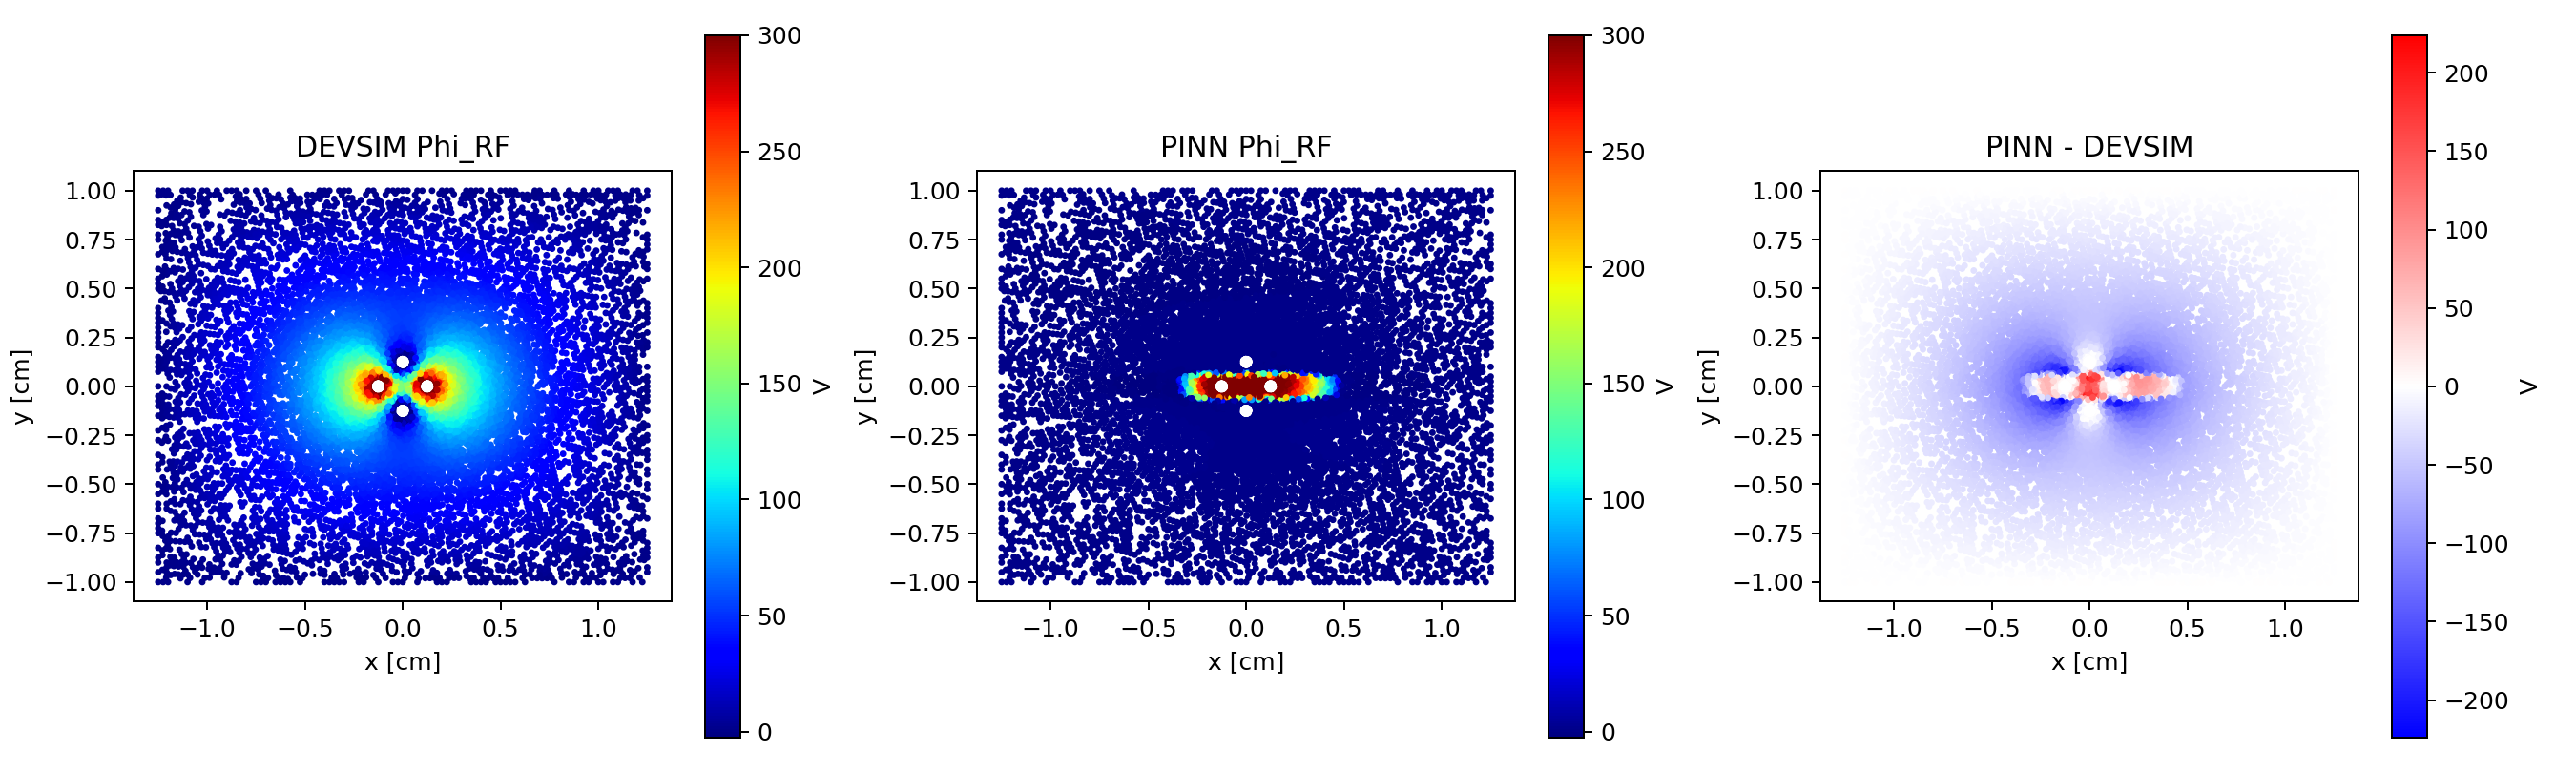
\includegraphics[width=\linewidth]{../runs/activation_pinn_20260602_015033_activation_relu/comparison_phi_rf.png}
\end{column}
\begin{column}{0.49\textwidth}
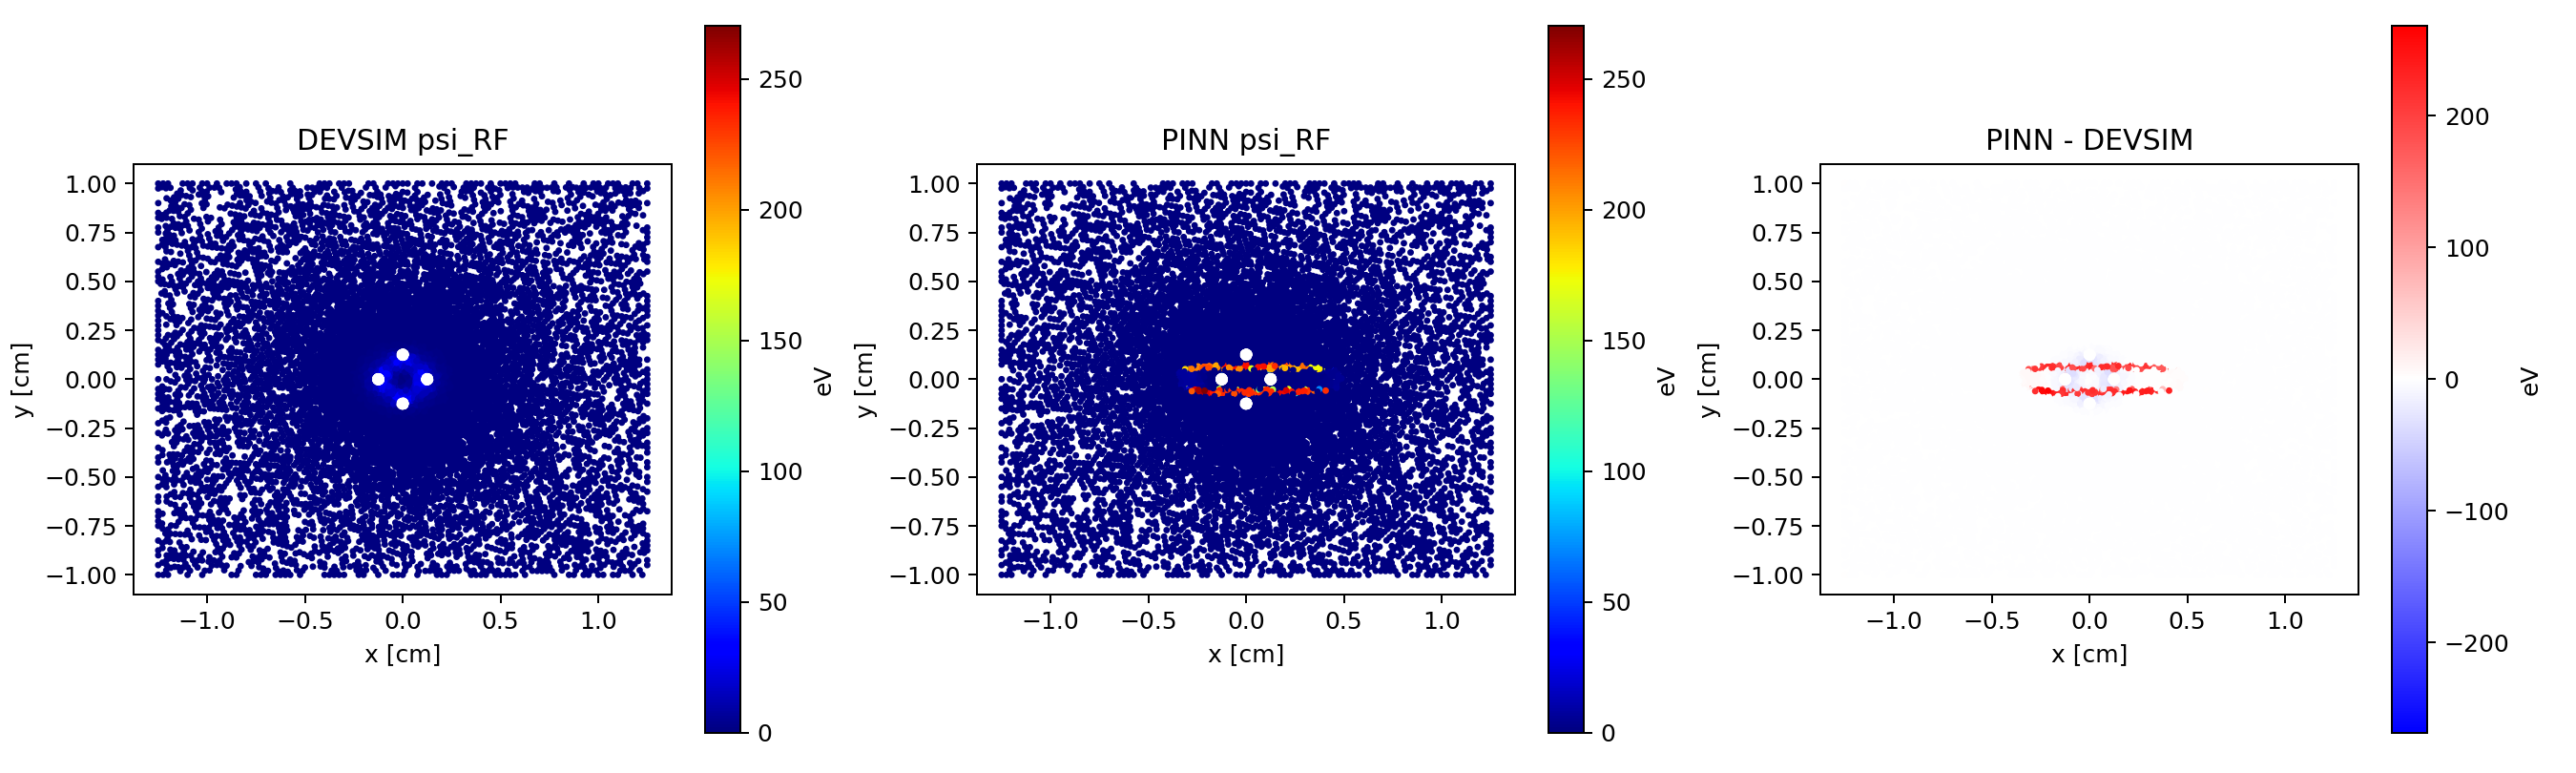
\includegraphics[width=\linewidth]{../runs/activation_pinn_20260602_015033_activation_relu/comparison_psi_rf_eV.png}
\end{column}
\end{columns}
\vspace{0.08in}
\small Misleading loss case: training loss collapses, but field error is the worst in the sweep.
\end{frame}

\begin{frame}[t]{activation\_sigmoid}
\begin{columns}[T,onlytextwidth]
\begin{column}{0.49\textwidth}
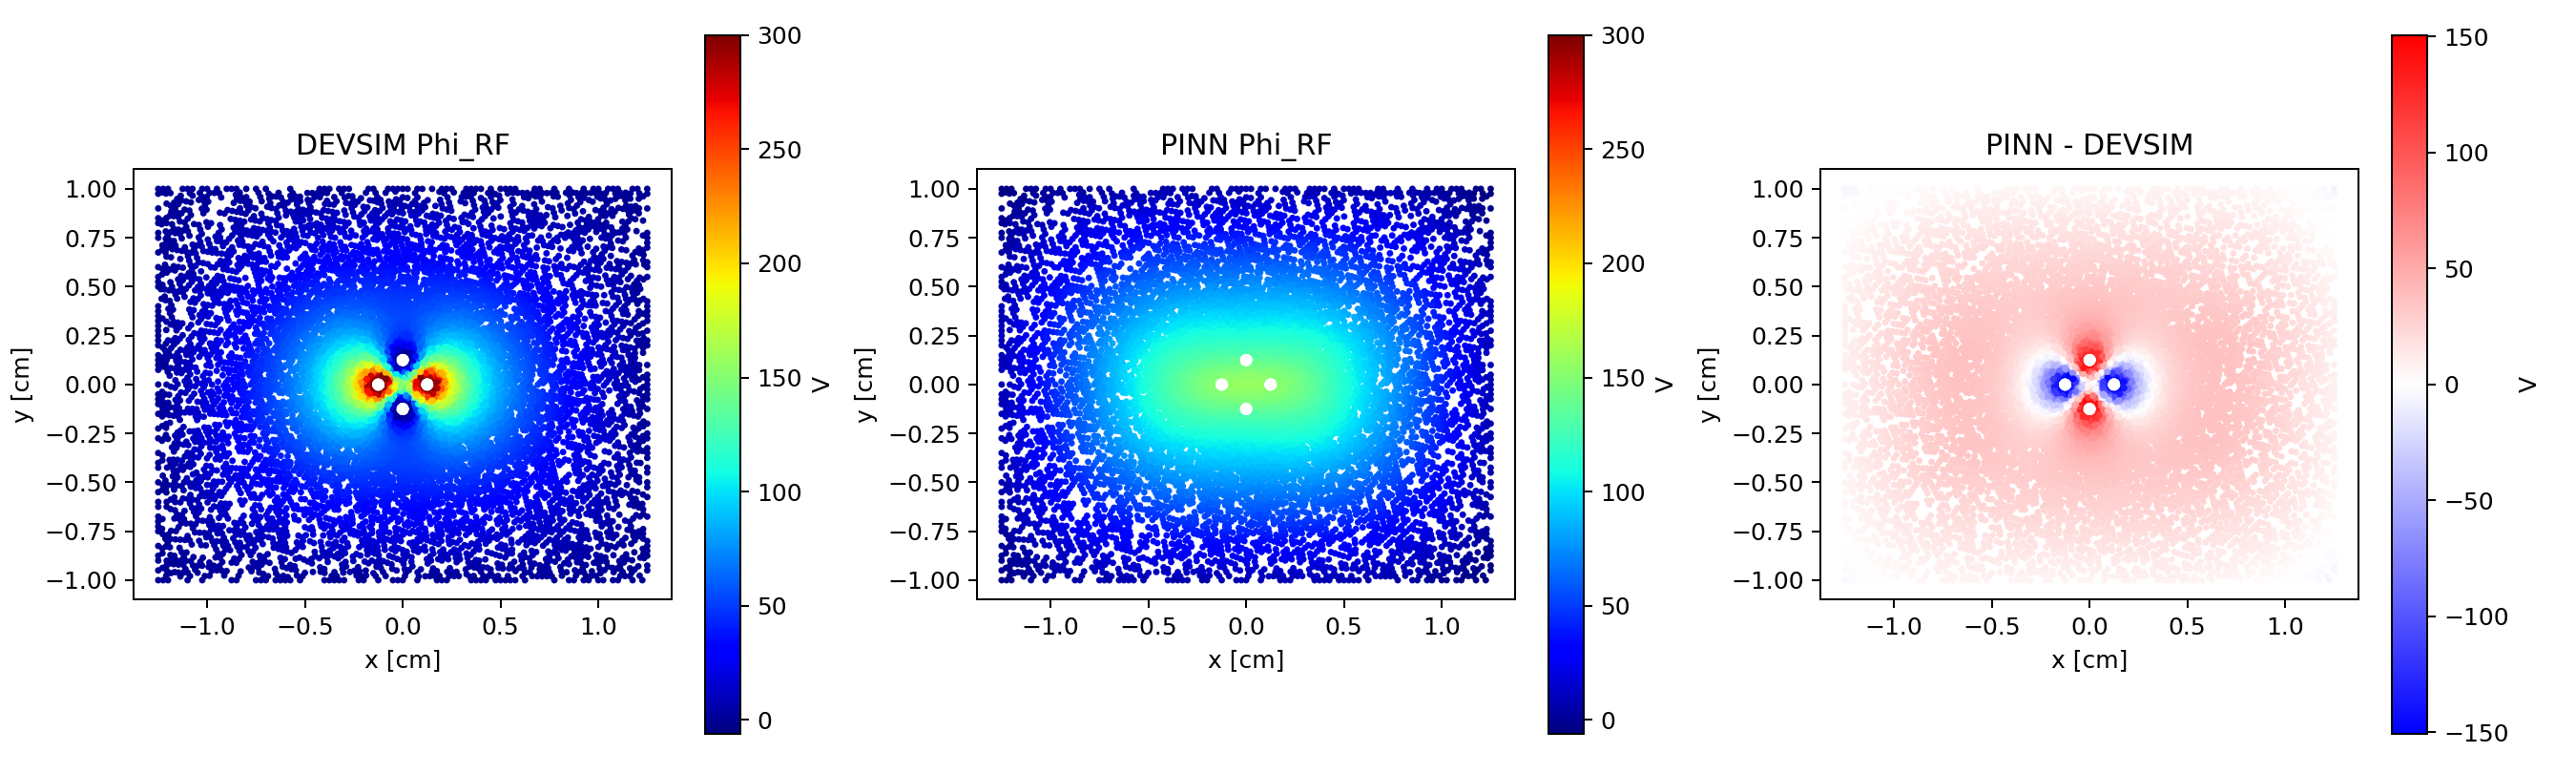
\includegraphics[width=\linewidth]{../runs/activation_pinn_20260602_015539_activation_sigmoid/comparison_phi_rf.png}
\end{column}
\begin{column}{0.49\textwidth}
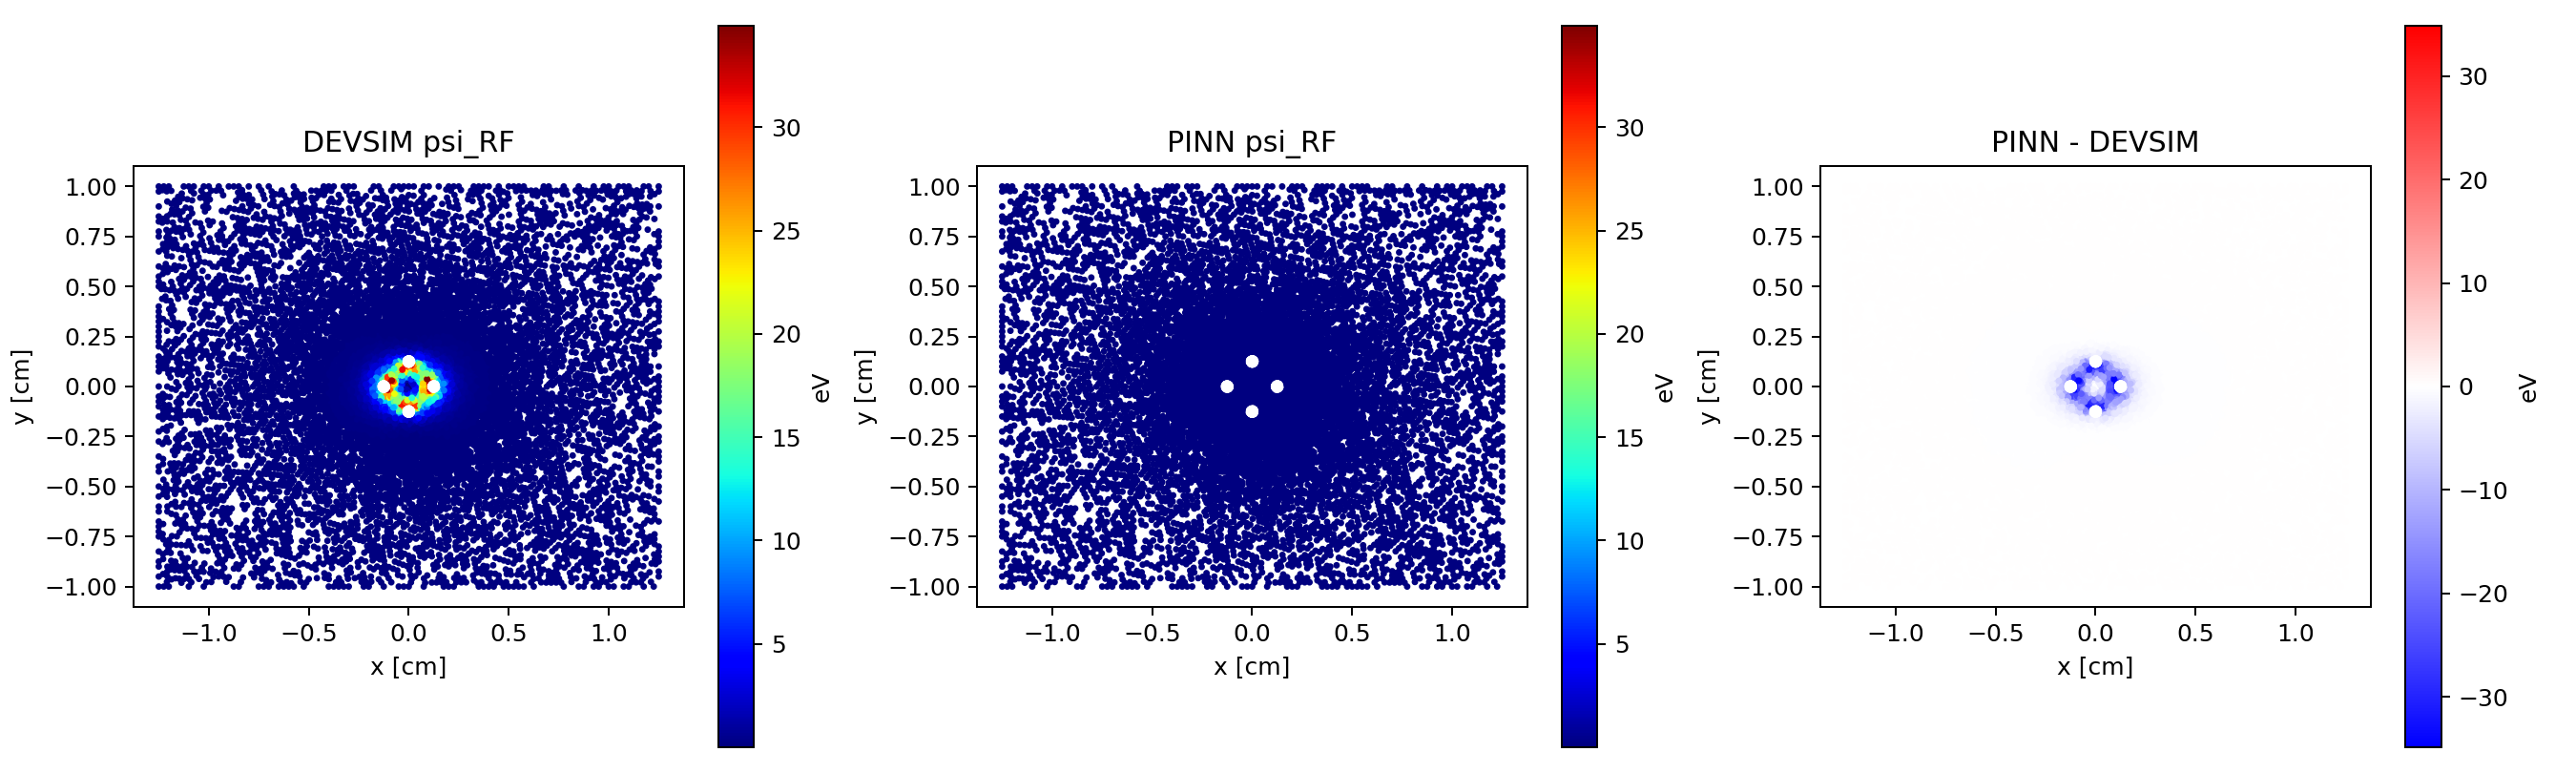
\includegraphics[width=\linewidth]{../runs/activation_pinn_20260602_015539_activation_sigmoid/comparison_psi_rf_eV.png}
\end{column}
\end{columns}
\vspace{0.08in}
\small Final normalized loss 0.486; Phi MSE 3.1e+03; Psi MSE 65.6.
\end{frame}

\begin{frame}[t]{activation\_sinusoidal}
\begin{columns}[T,onlytextwidth]
\begin{column}{0.49\textwidth}
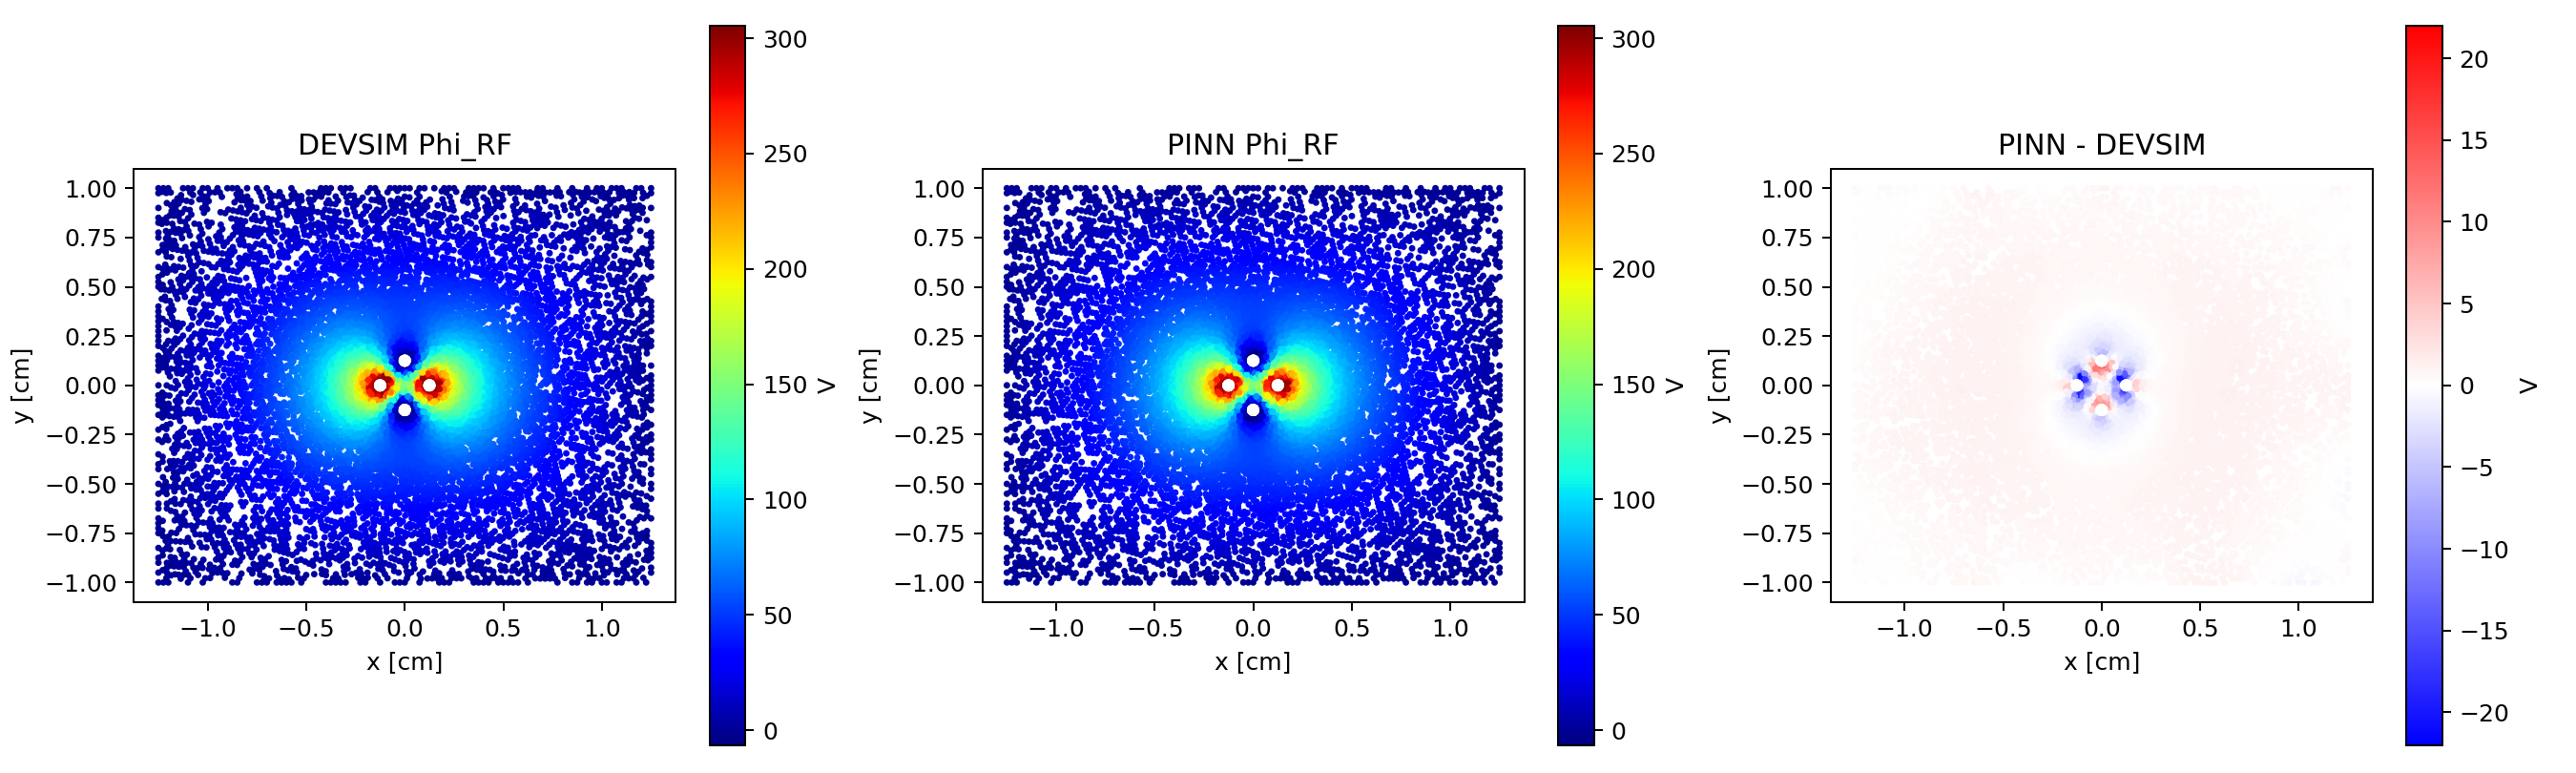
\includegraphics[width=\linewidth]{../runs/activation_pinn_20260602_020551_activation_sinusoidal/comparison_phi_rf.png}
\end{column}
\begin{column}{0.49\textwidth}
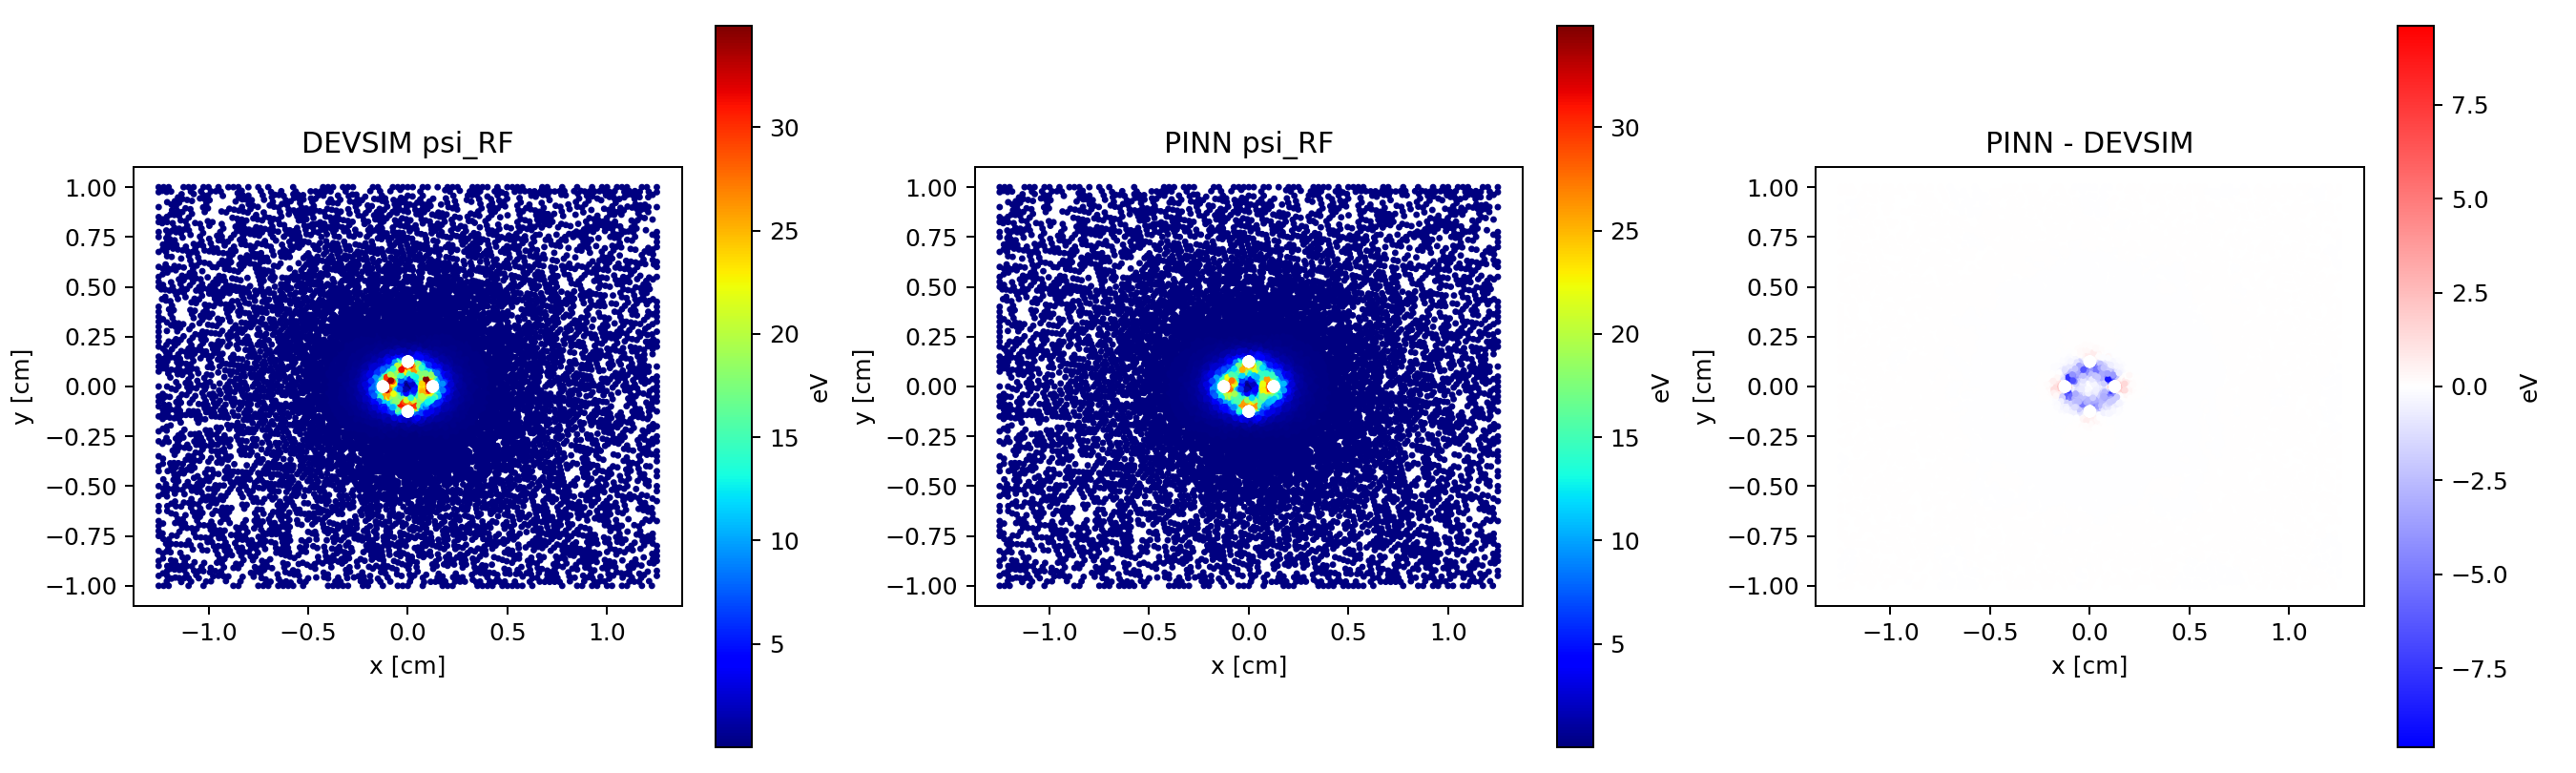
\includegraphics[width=\linewidth]{../runs/activation_pinn_20260602_020551_activation_sinusoidal/comparison_psi_rf_eV.png}
\end{column}
\end{columns}
\vspace{0.08in}
\small Best activation-only result; smooth derivatives help the PDE residual and gradient-derived Psi.
\end{frame}

\begin{frame}[t]{baseline}
\begin{columns}[T,onlytextwidth]
\begin{column}{0.49\textwidth}
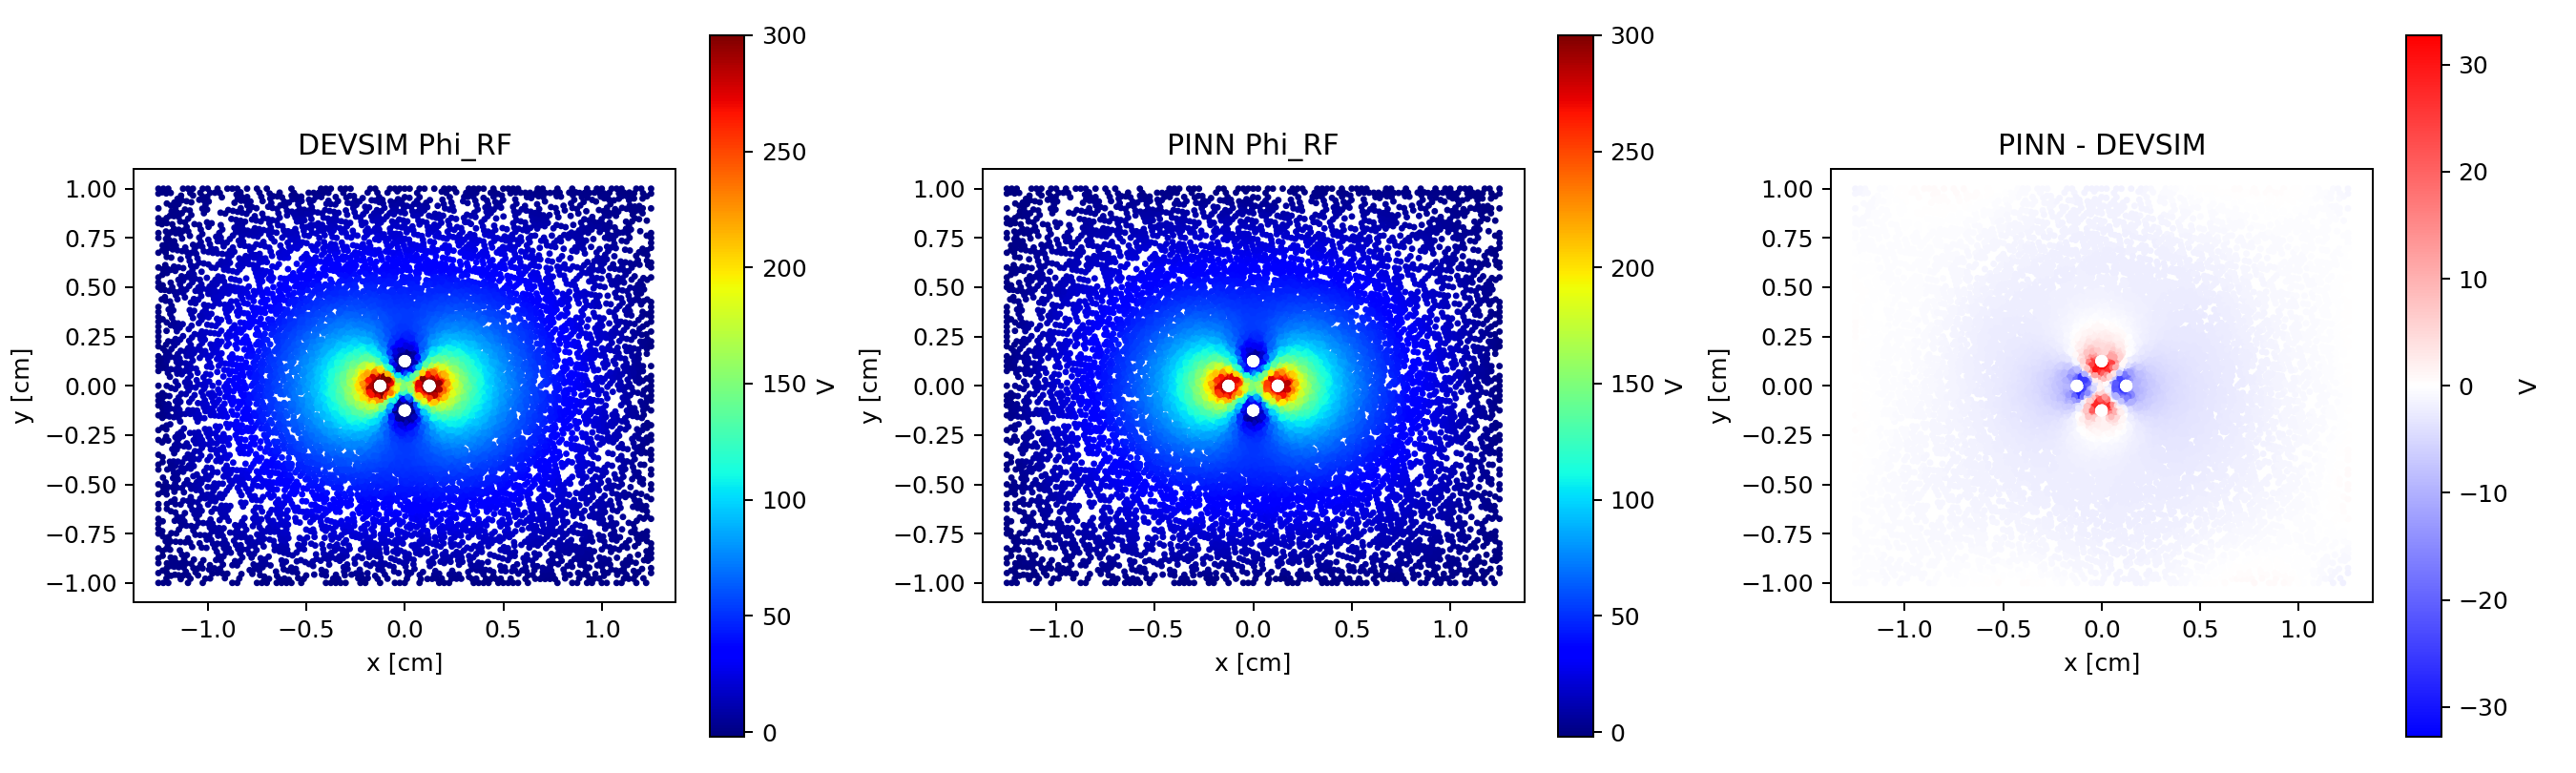
\includegraphics[width=\linewidth]{../runs/baseline_pinn_20260602_000649_baseline/comparison_phi_rf.png}
\end{column}
\begin{column}{0.49\textwidth}
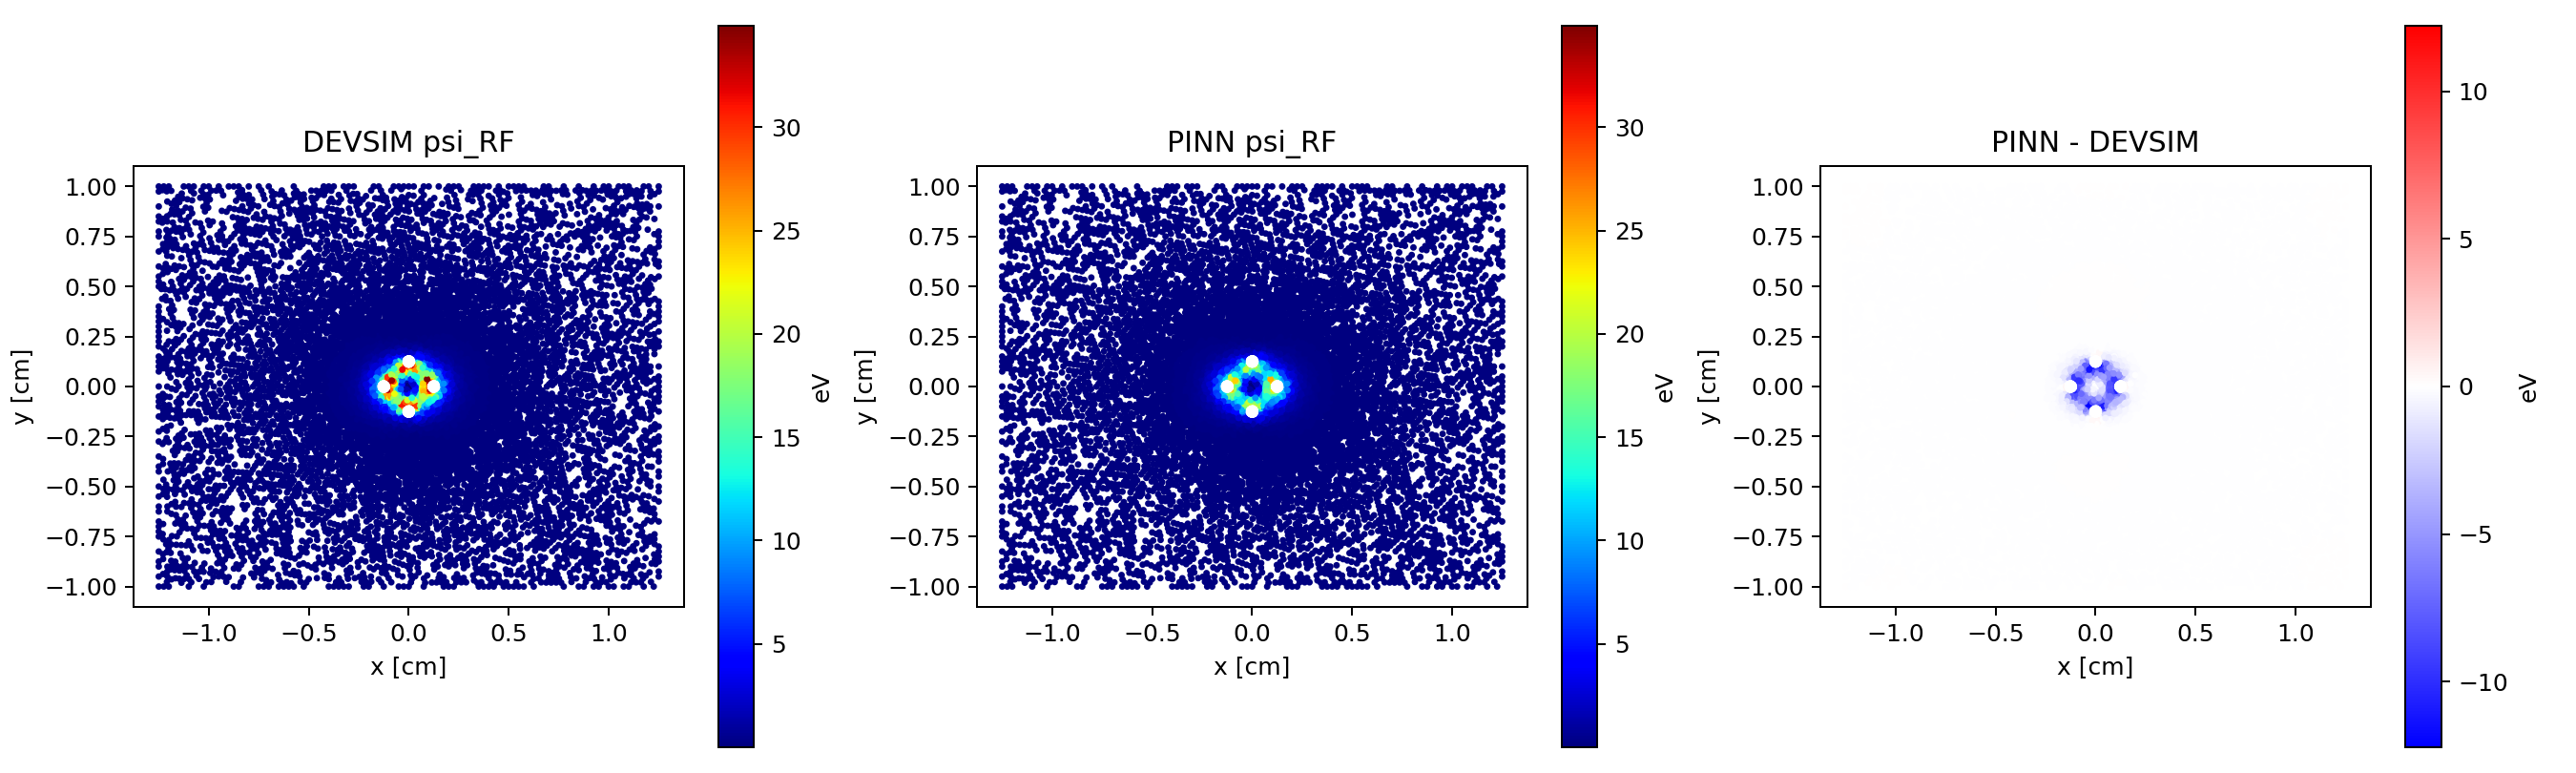
\includegraphics[width=\linewidth]{../runs/baseline_pinn_20260602_000649_baseline/comparison_psi_rf_eV.png}
\end{column}
\end{columns}
\vspace{0.08in}
\small Reference run for all hyperparameter comparisons.
\end{frame}

\begin{frame}[t]{bc\_weight\_1}
\begin{columns}[T,onlytextwidth]
\begin{column}{0.49\textwidth}
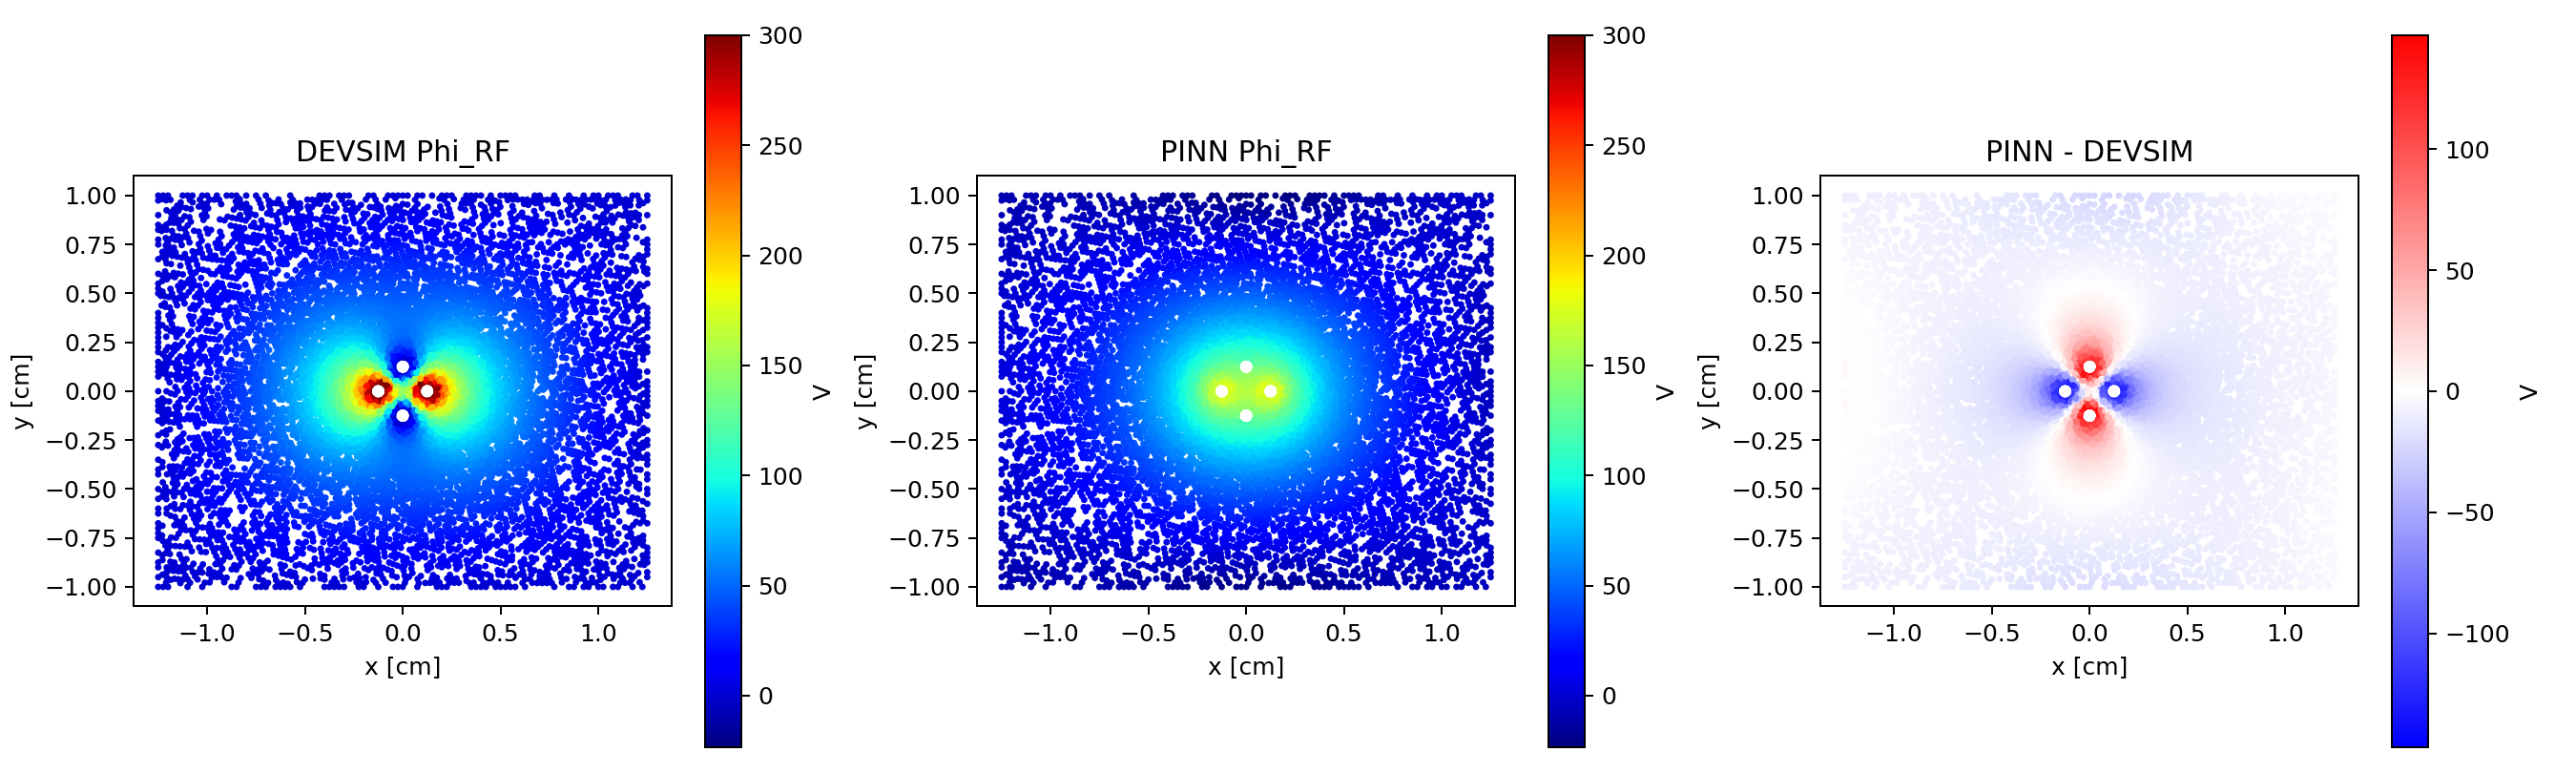
\includegraphics[width=\linewidth]{../runs/bc_weight_pinn_20260602_021939_bc_weight_1/comparison_phi_rf.png}
\end{column}
\begin{column}{0.49\textwidth}
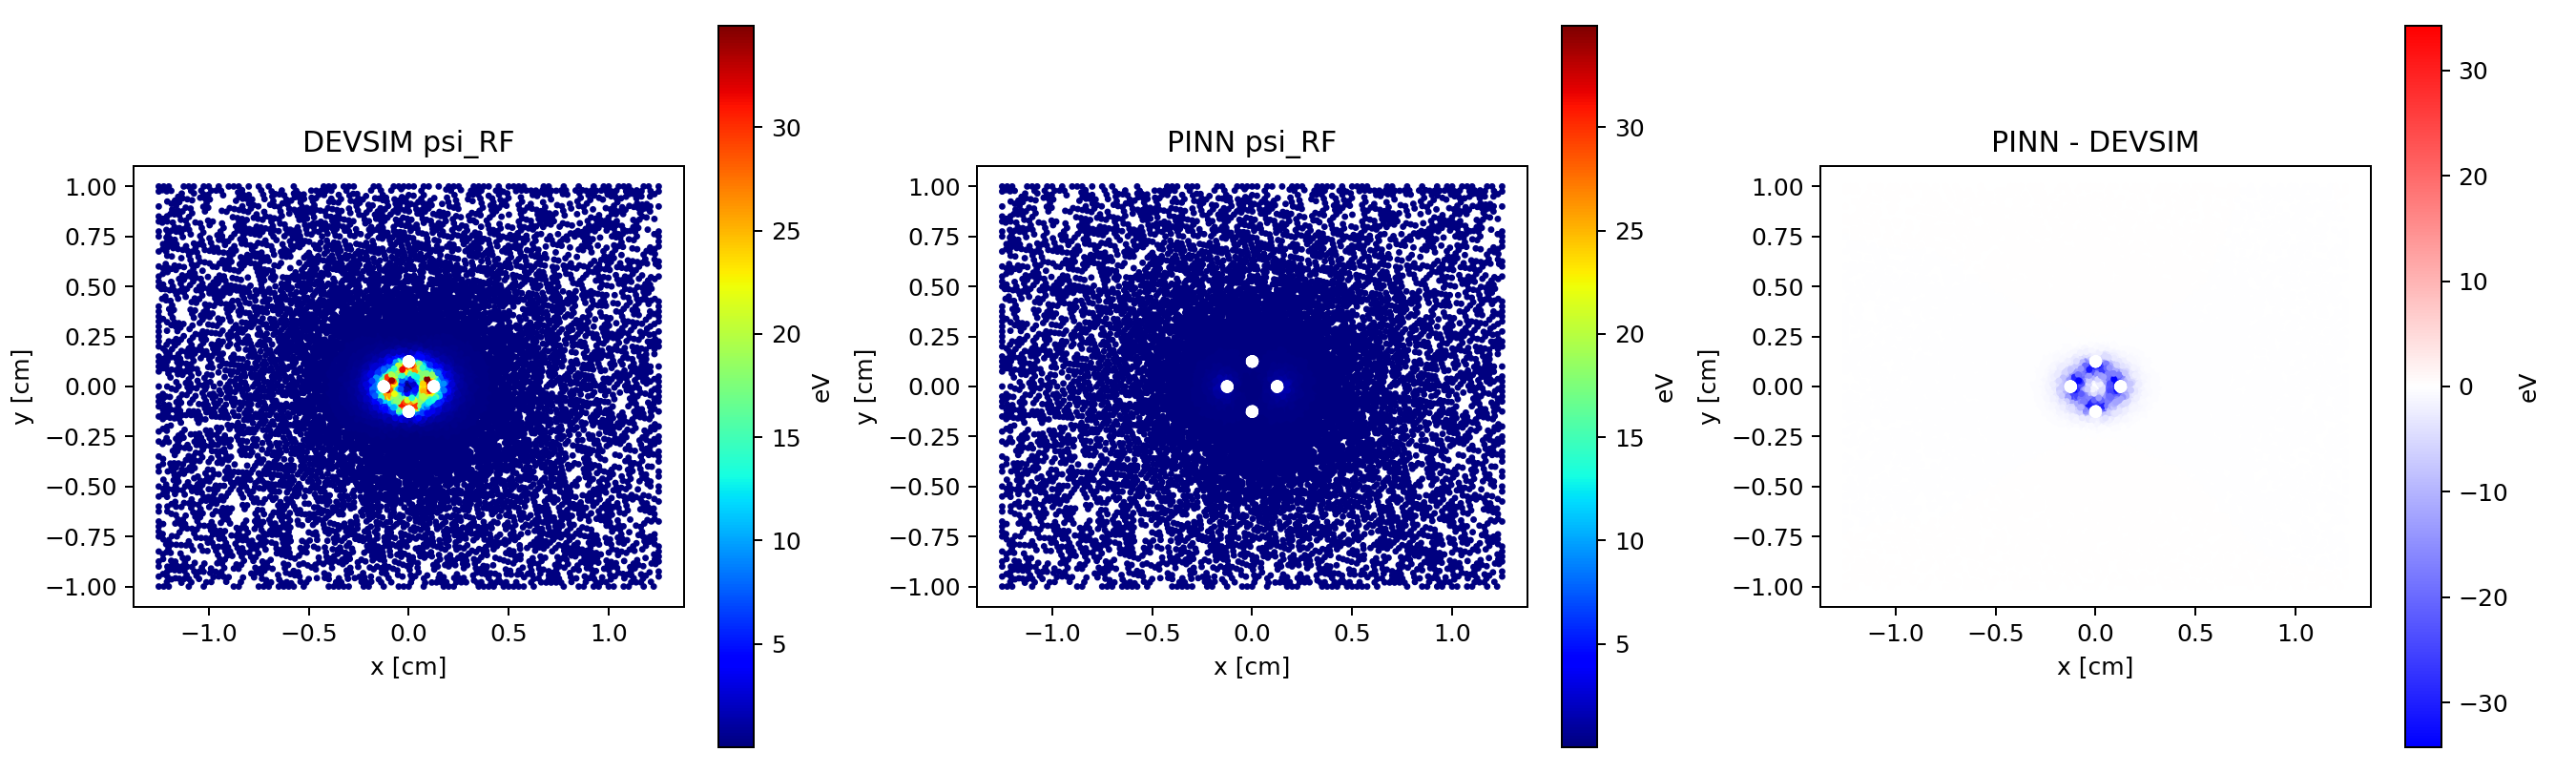
\includegraphics[width=\linewidth]{../runs/bc_weight_pinn_20260602_021939_bc_weight_1/comparison_psi_rf_eV.png}
\end{column}
\end{columns}
\vspace{0.08in}
\small Final normalized loss 0.379; Phi MSE 2.44e+03; Psi MSE 63.1.
\end{frame}

\begin{frame}[t]{bc\_weight\_10}
\begin{columns}[T,onlytextwidth]
\begin{column}{0.49\textwidth}
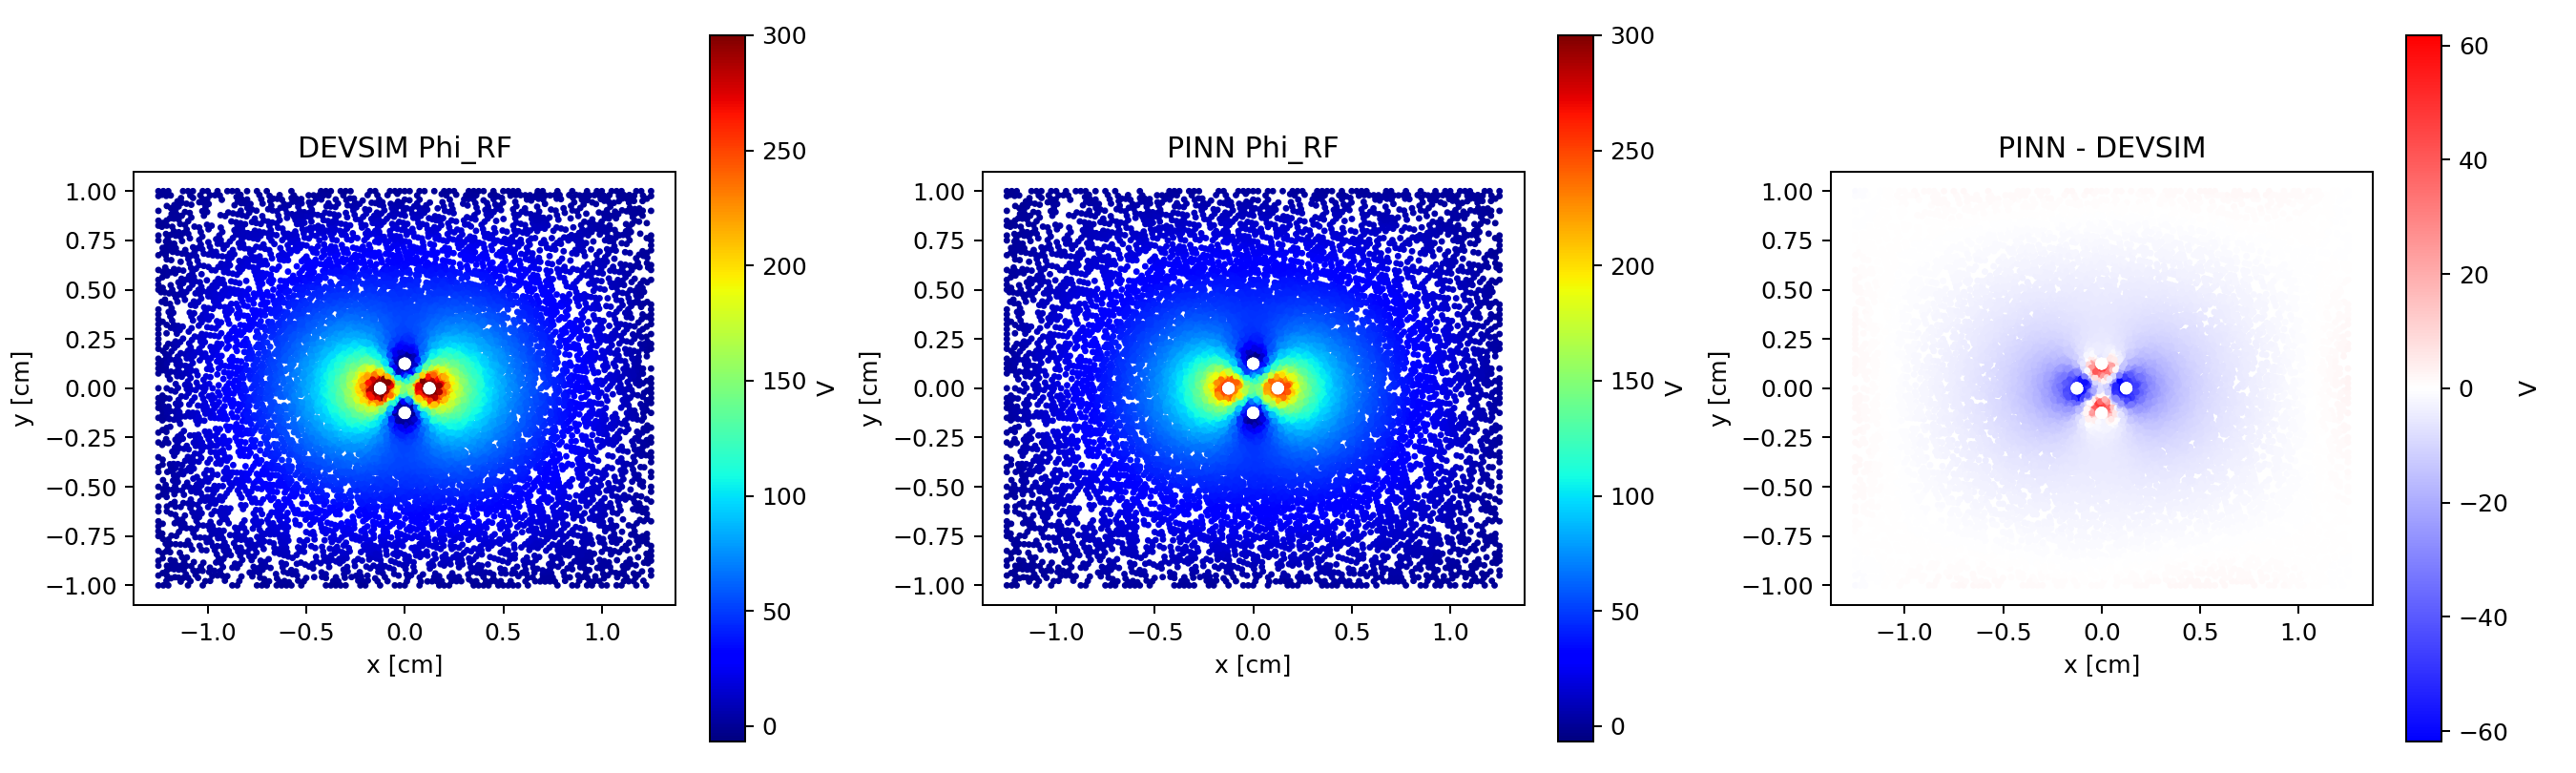
\includegraphics[width=\linewidth]{../runs/bc_weight_pinn_20260602_023047_bc_weight_10/comparison_phi_rf.png}
\end{column}
\begin{column}{0.49\textwidth}
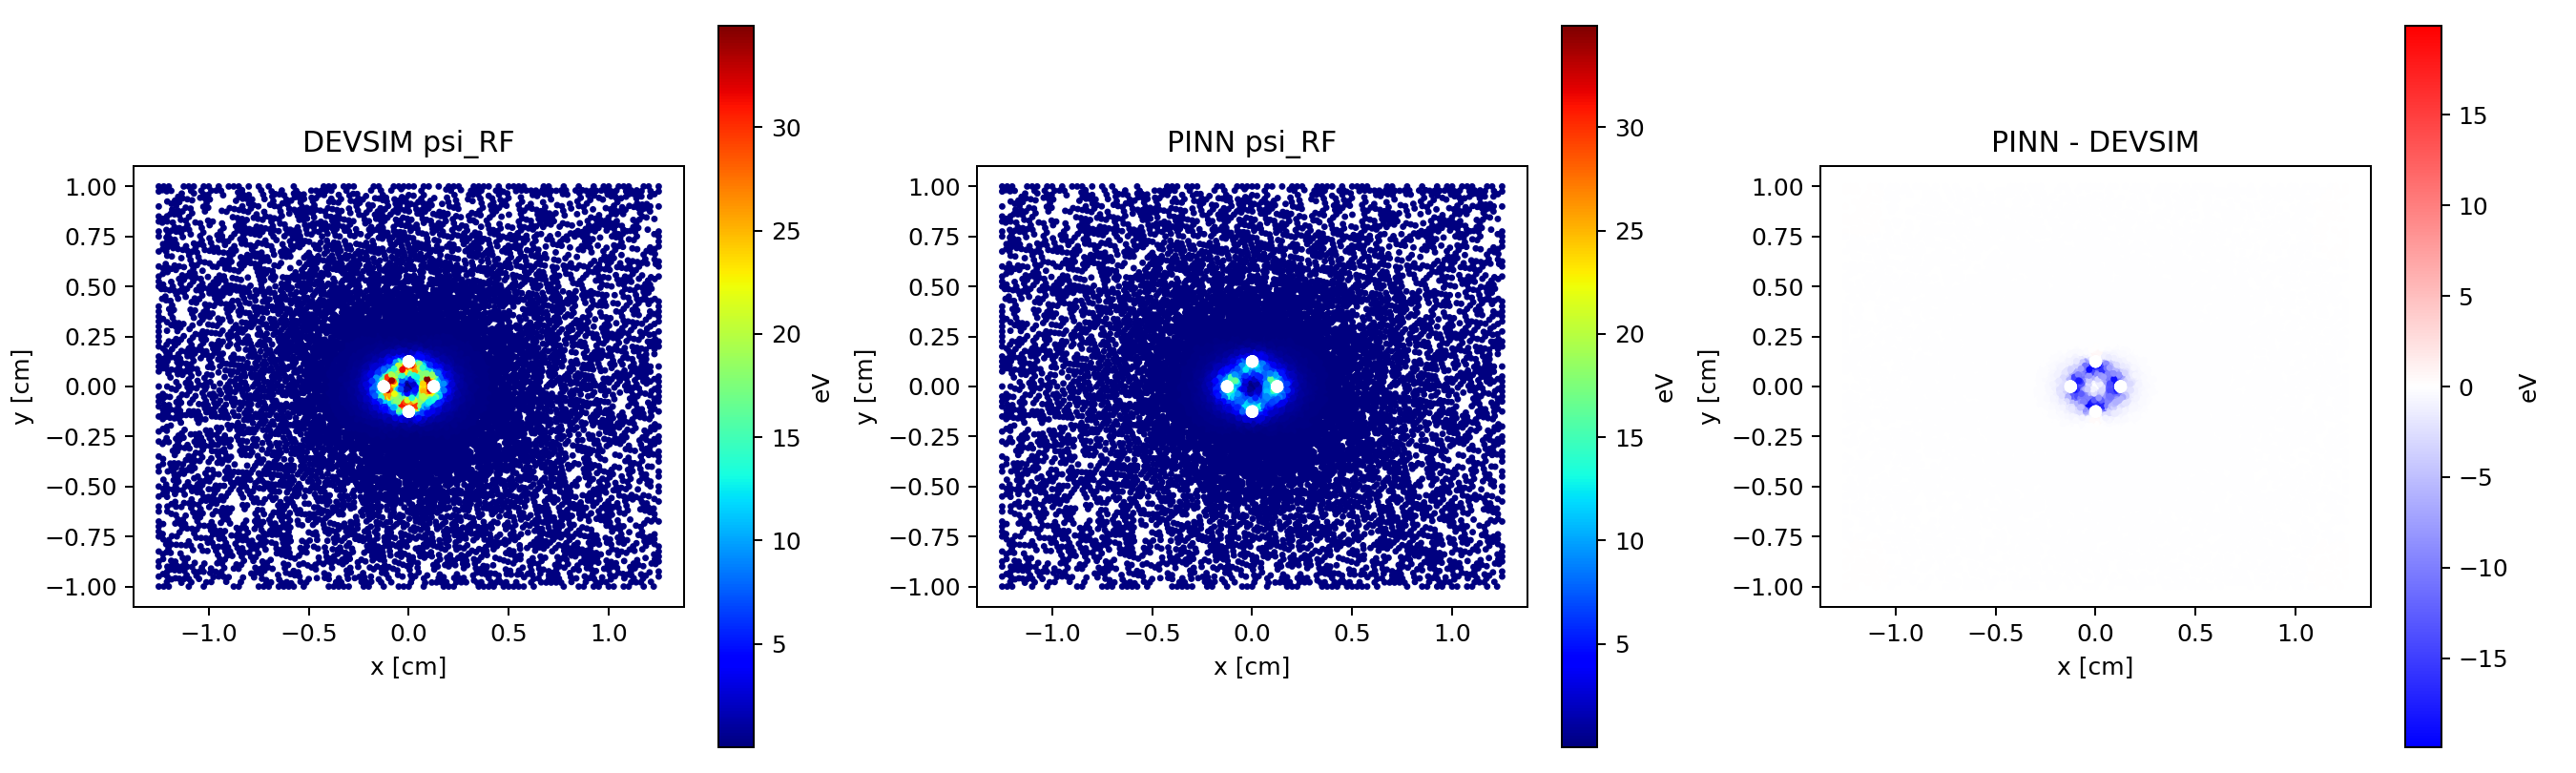
\includegraphics[width=\linewidth]{../runs/bc_weight_pinn_20260602_023047_bc_weight_10/comparison_psi_rf_eV.png}
\end{column}
\end{columns}
\vspace{0.08in}
\small Final normalized loss 0.0814; Phi MSE 335; Psi MSE 19.3.
\end{frame}

\begin{frame}[t]{bc\_weight\_1000}
\begin{columns}[T,onlytextwidth]
\begin{column}{0.49\textwidth}
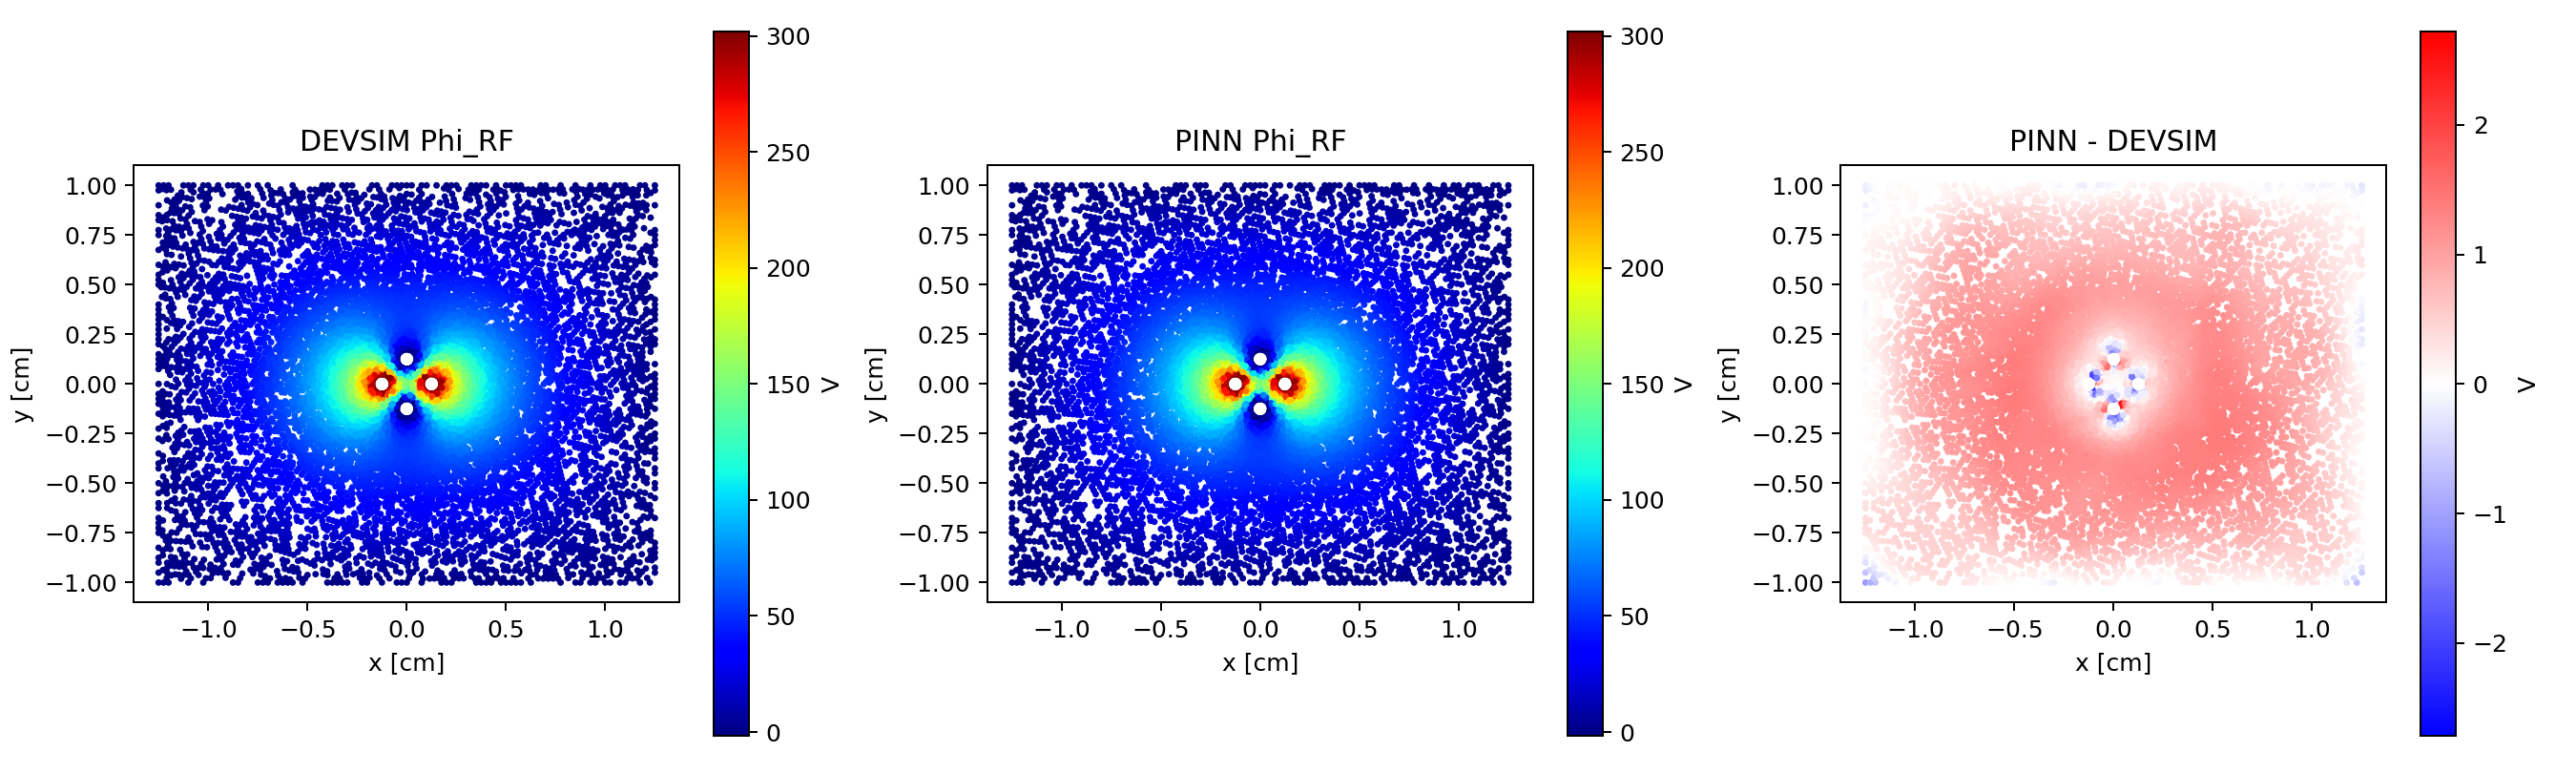
\includegraphics[width=\linewidth]{../runs/bc_weight_pinn_20260602_024202_bc_weight_1000/comparison_phi_rf.png}
\end{column}
\begin{column}{0.49\textwidth}
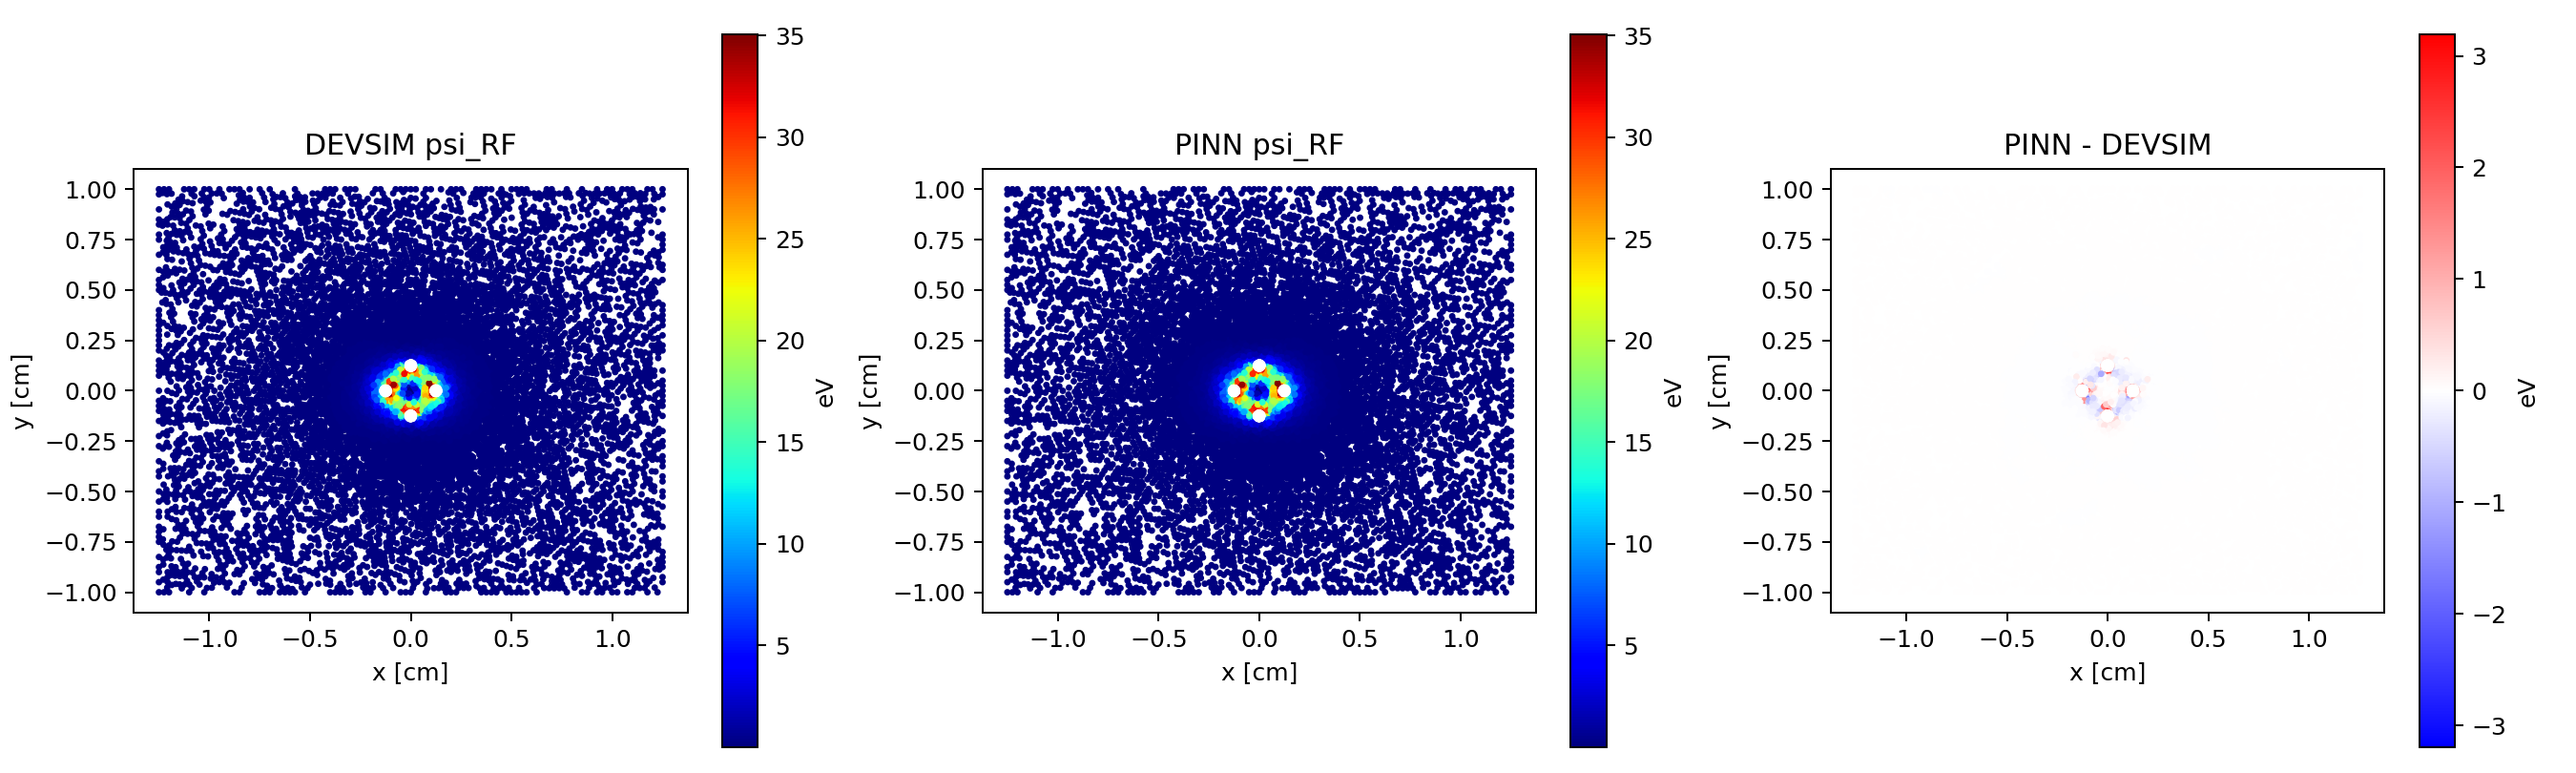
\includegraphics[width=\linewidth]{../runs/bc_weight_pinn_20260602_024202_bc_weight_1000/comparison_psi_rf_eV.png}
\end{column}
\end{columns}
\vspace{0.08in}
\small Best overall DEVSIM match; strong boundary enforcement did not destroy field accuracy.
\end{frame}

\begin{frame}[t]{depth\_2}
\begin{columns}[T,onlytextwidth]
\begin{column}{0.49\textwidth}
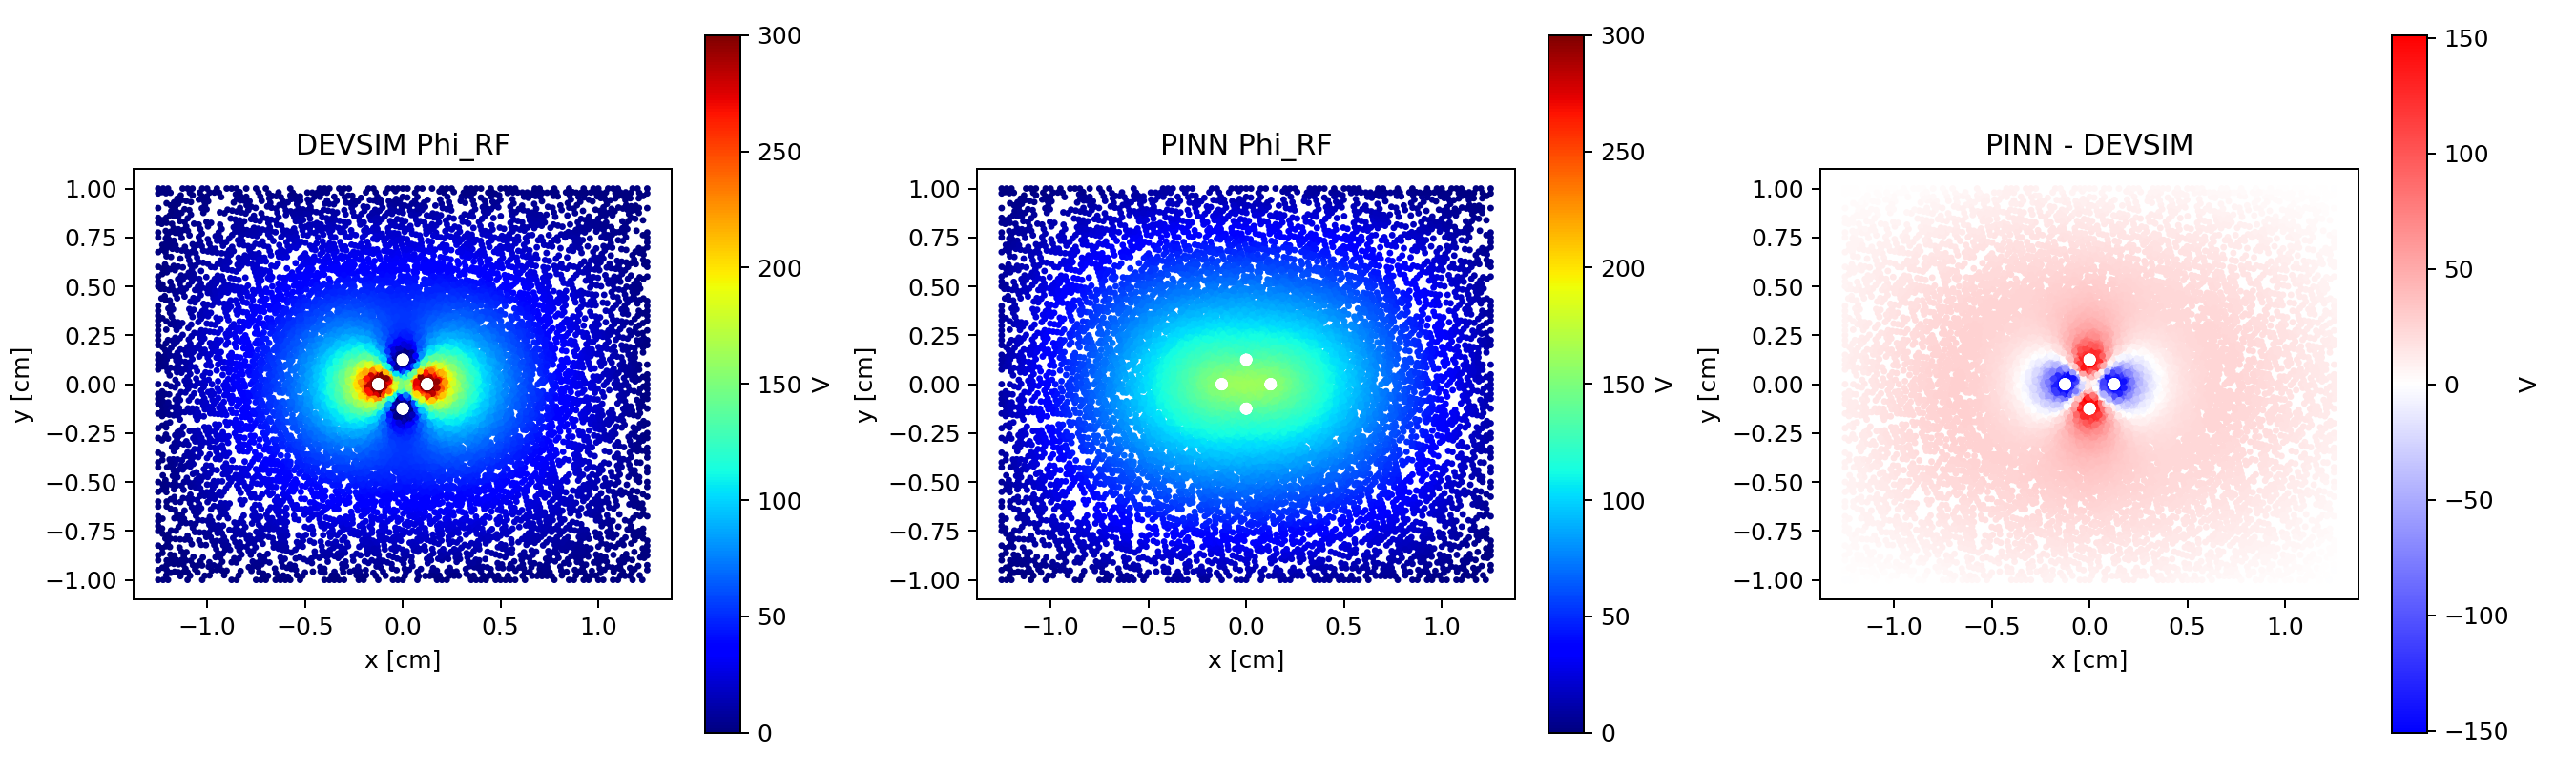
\includegraphics[width=\linewidth]{../runs/depth_pinn_20260602_005521_depth_2/comparison_phi_rf.png}
\end{column}
\begin{column}{0.49\textwidth}
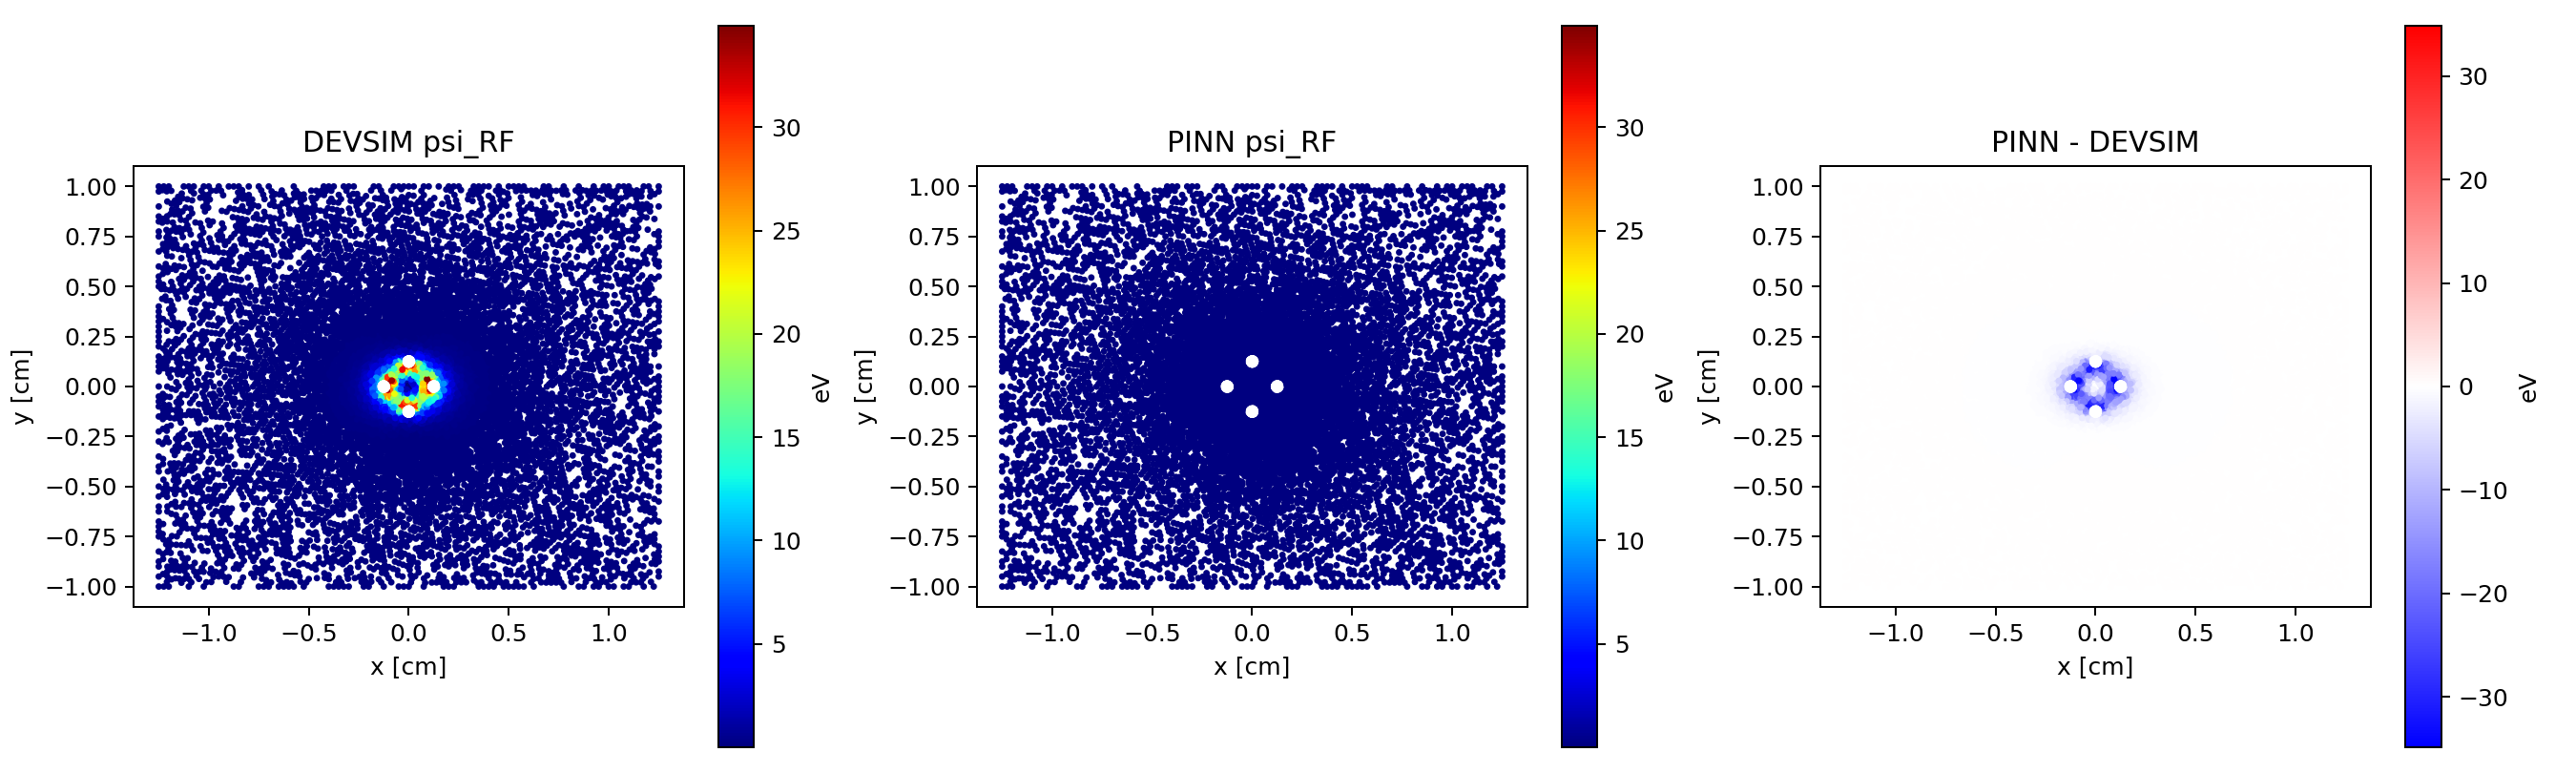
\includegraphics[width=\linewidth]{../runs/depth_pinn_20260602_005521_depth_2/comparison_psi_rf_eV.png}
\end{column}
\end{columns}
\vspace{0.08in}
\small Final normalized loss 0.478; Phi MSE 2.95e+03; Psi MSE 65.4.
\end{frame}

\begin{frame}[t]{depth\_6}
\begin{columns}[T,onlytextwidth]
\begin{column}{0.49\textwidth}
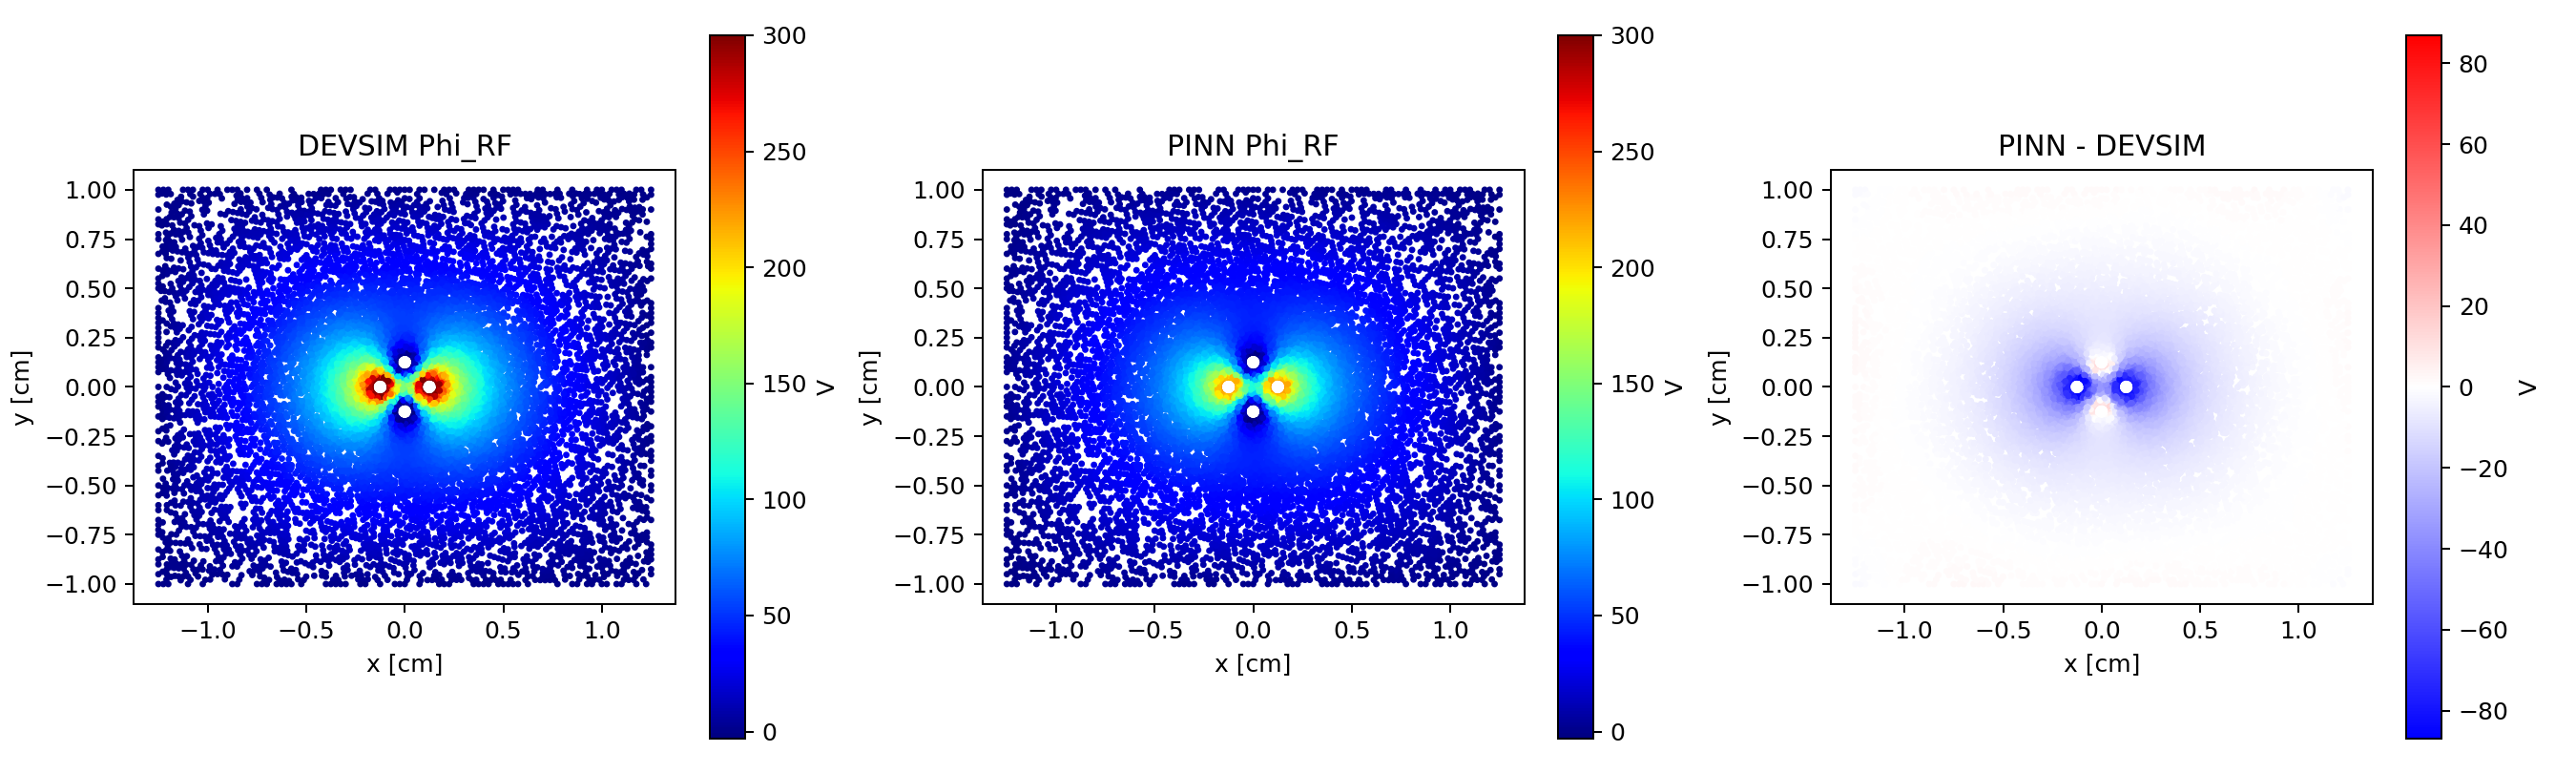
\includegraphics[width=\linewidth]{../runs/depth_pinn_20260602_010505_depth_6/comparison_phi_rf.png}
\end{column}
\begin{column}{0.49\textwidth}
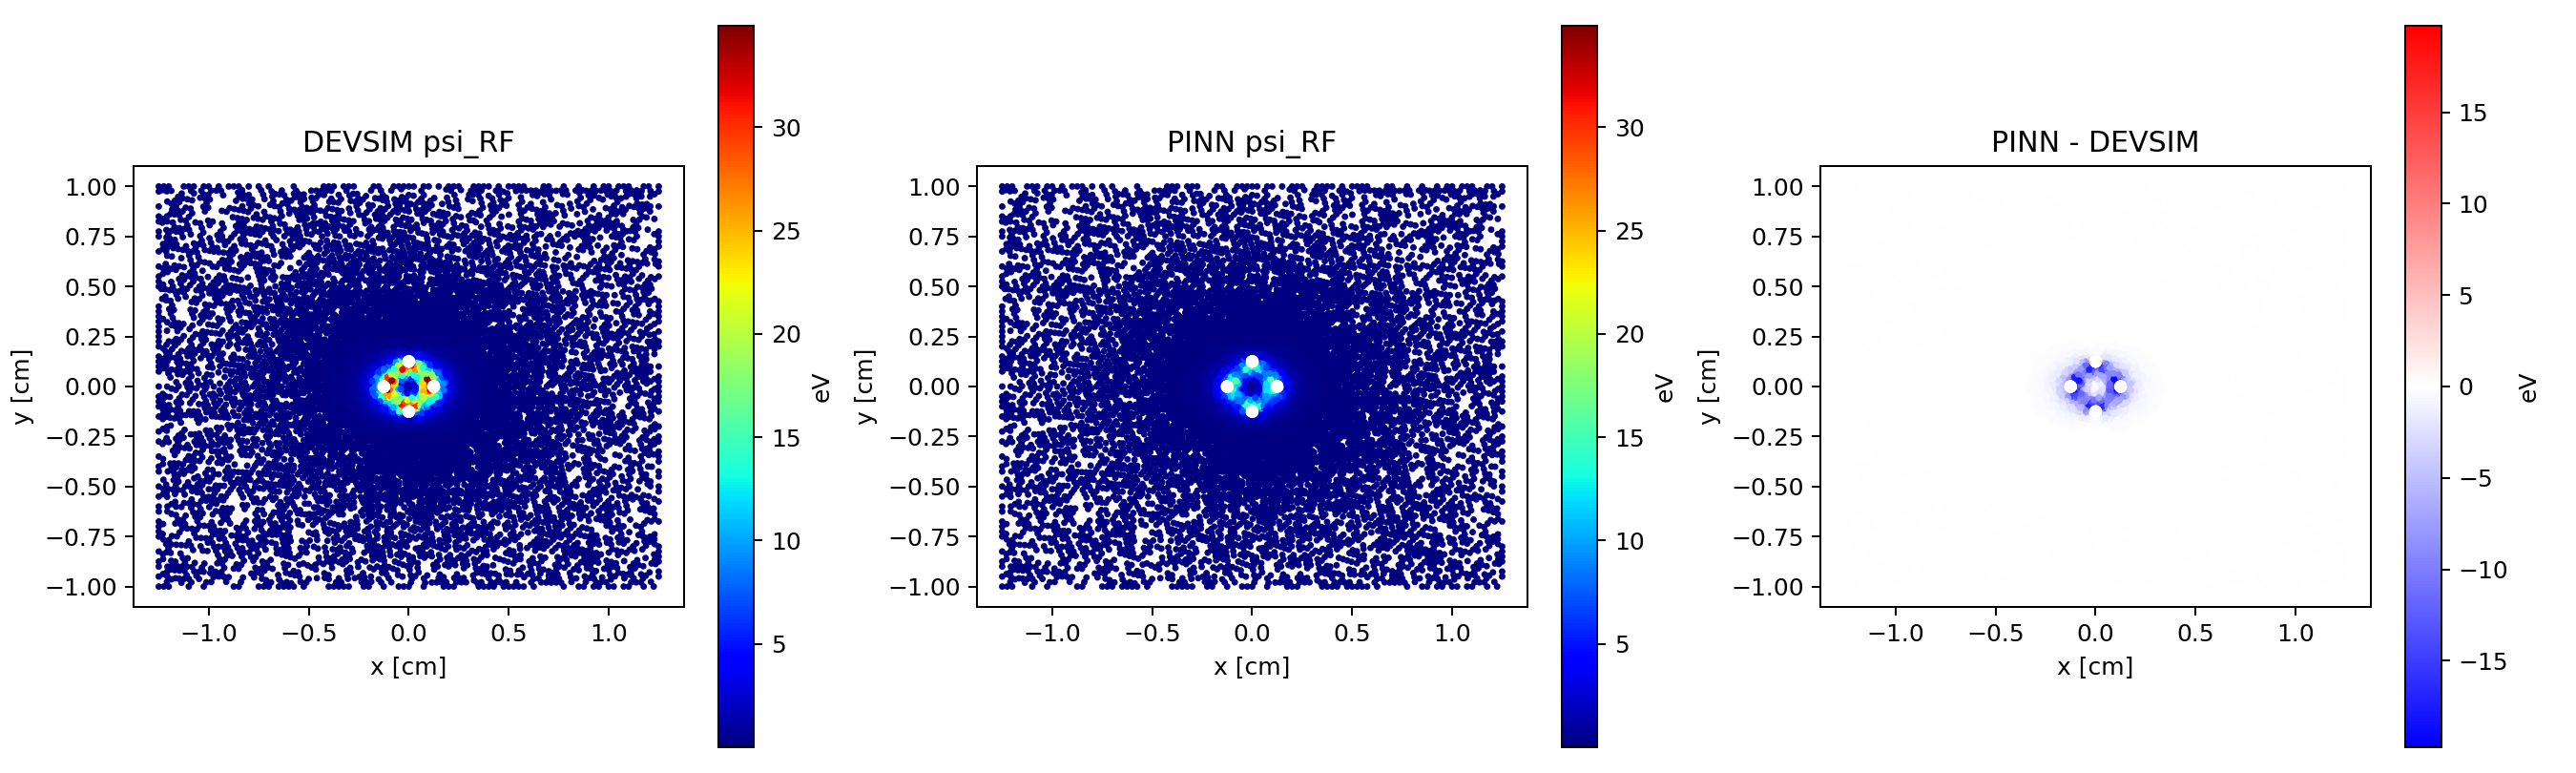
\includegraphics[width=\linewidth]{../runs/depth_pinn_20260602_010505_depth_6/comparison_psi_rf_eV.png}
\end{column}
\end{columns}
\vspace{0.08in}
\small Final normalized loss 2.4; Phi MSE 886; Psi MSE 18.3.
\end{frame}

\begin{frame}[t]{depth\_8}
\begin{columns}[T,onlytextwidth]
\begin{column}{0.49\textwidth}
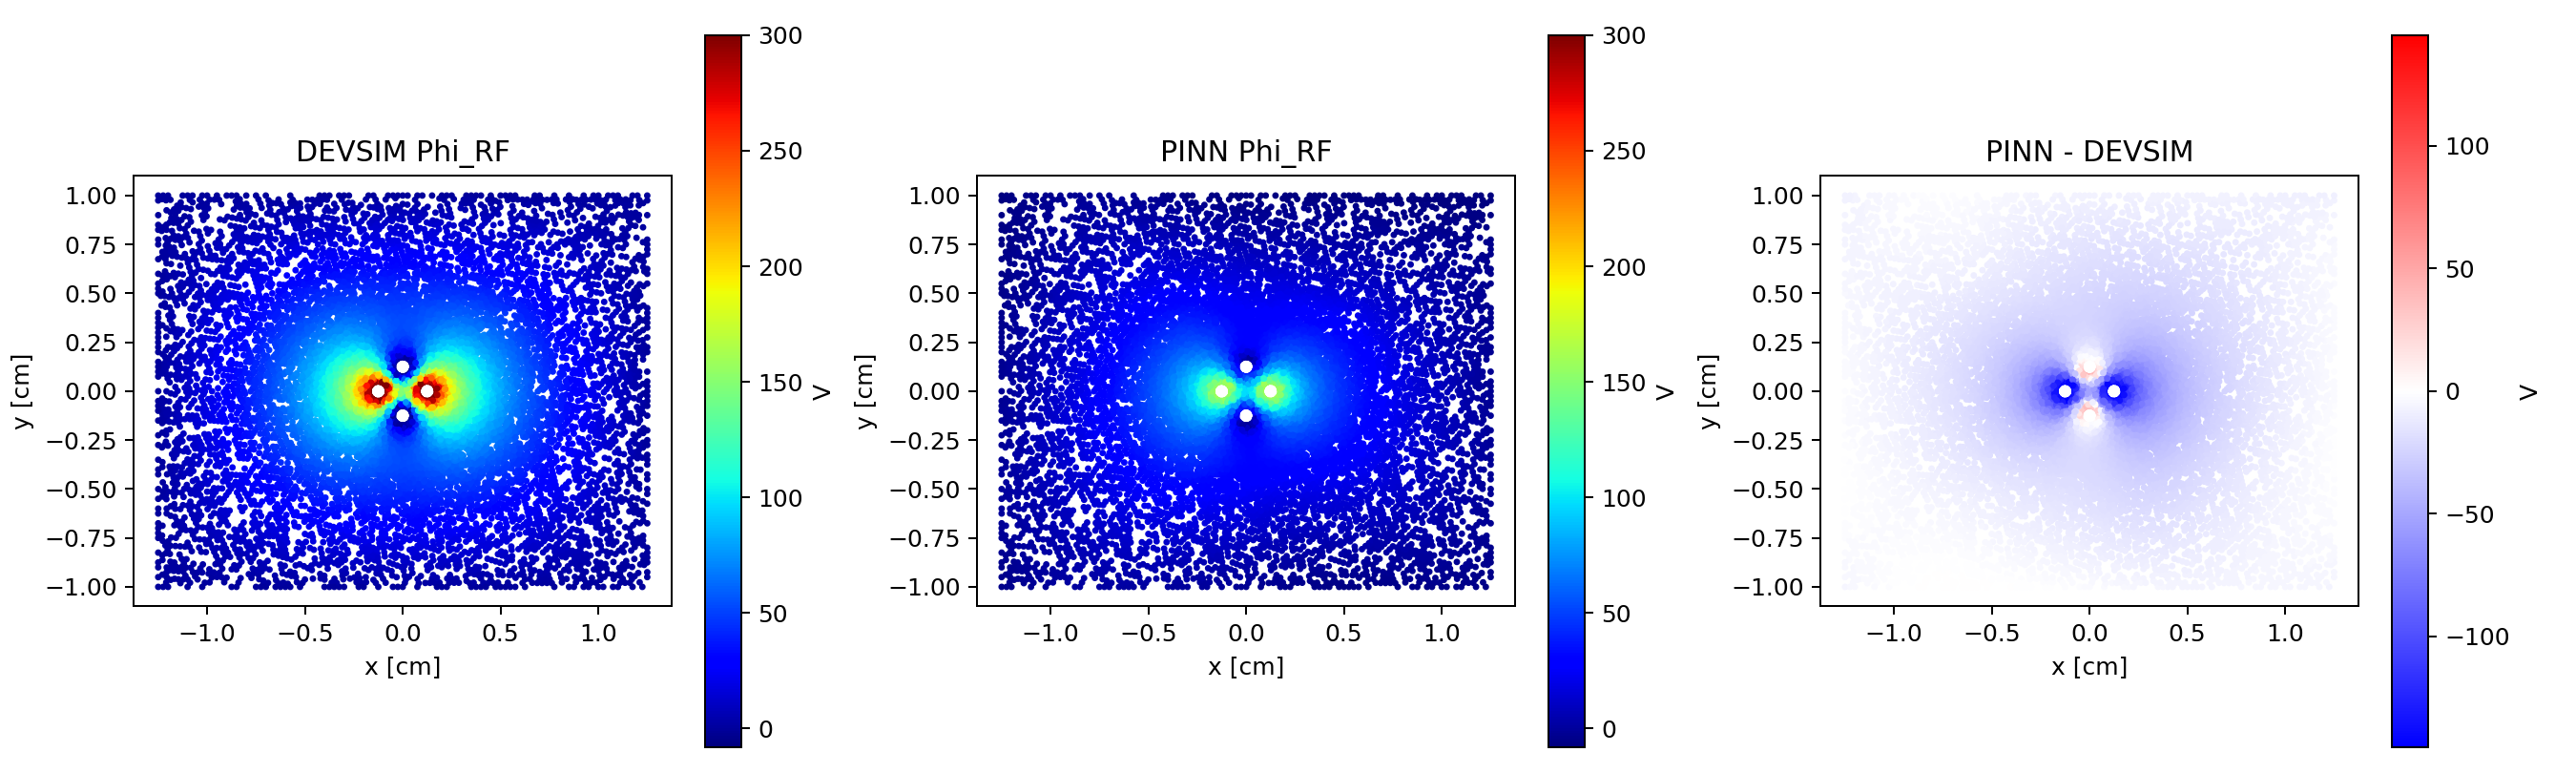
\includegraphics[width=\linewidth]{../runs/depth_pinn_20260602_012632_depth_8/comparison_phi_rf.png}
\end{column}
\begin{column}{0.49\textwidth}
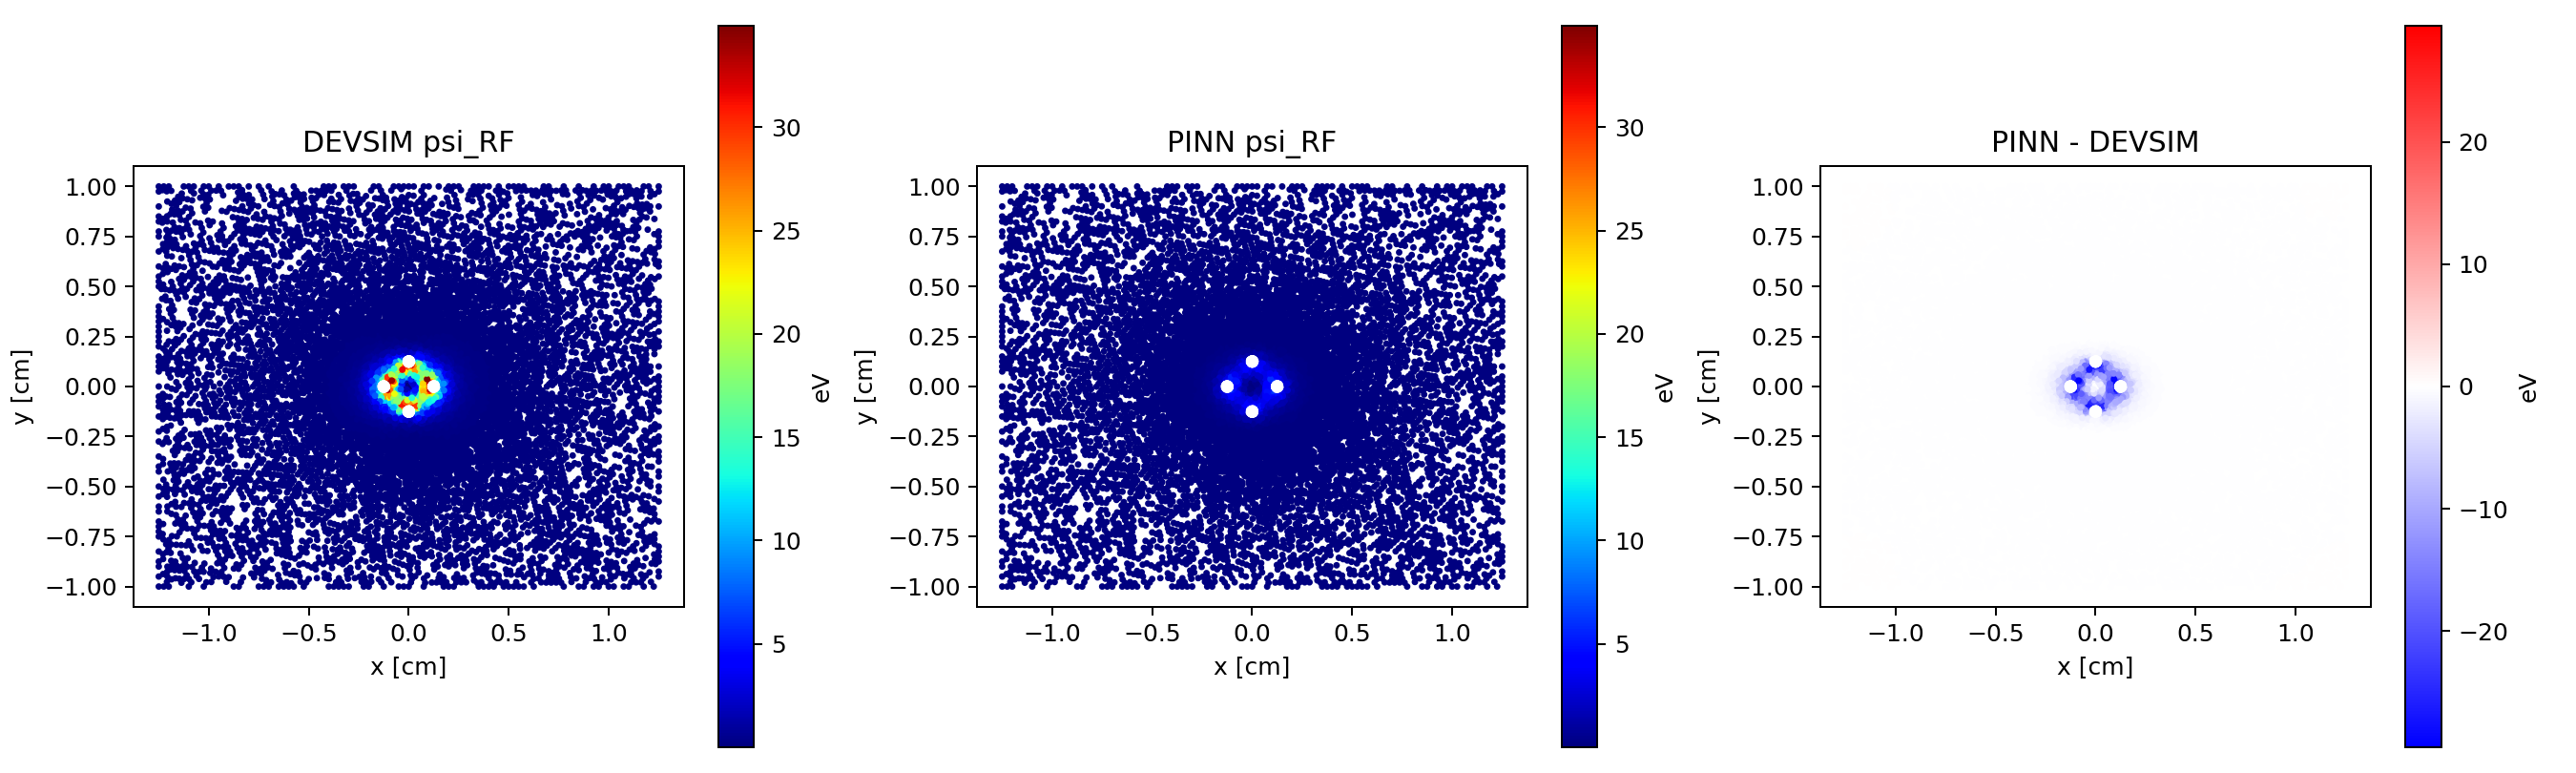
\includegraphics[width=\linewidth]{../runs/depth_pinn_20260602_012632_depth_8/comparison_psi_rf_eV.png}
\end{column}
\end{columns}
\vspace{0.08in}
\small Final normalized loss 3.41; Phi MSE 2.81e+03; Psi MSE 44.4.
\end{frame}

\begin{frame}[t]{lr\_1e-4}
\begin{columns}[T,onlytextwidth]
\begin{column}{0.49\textwidth}
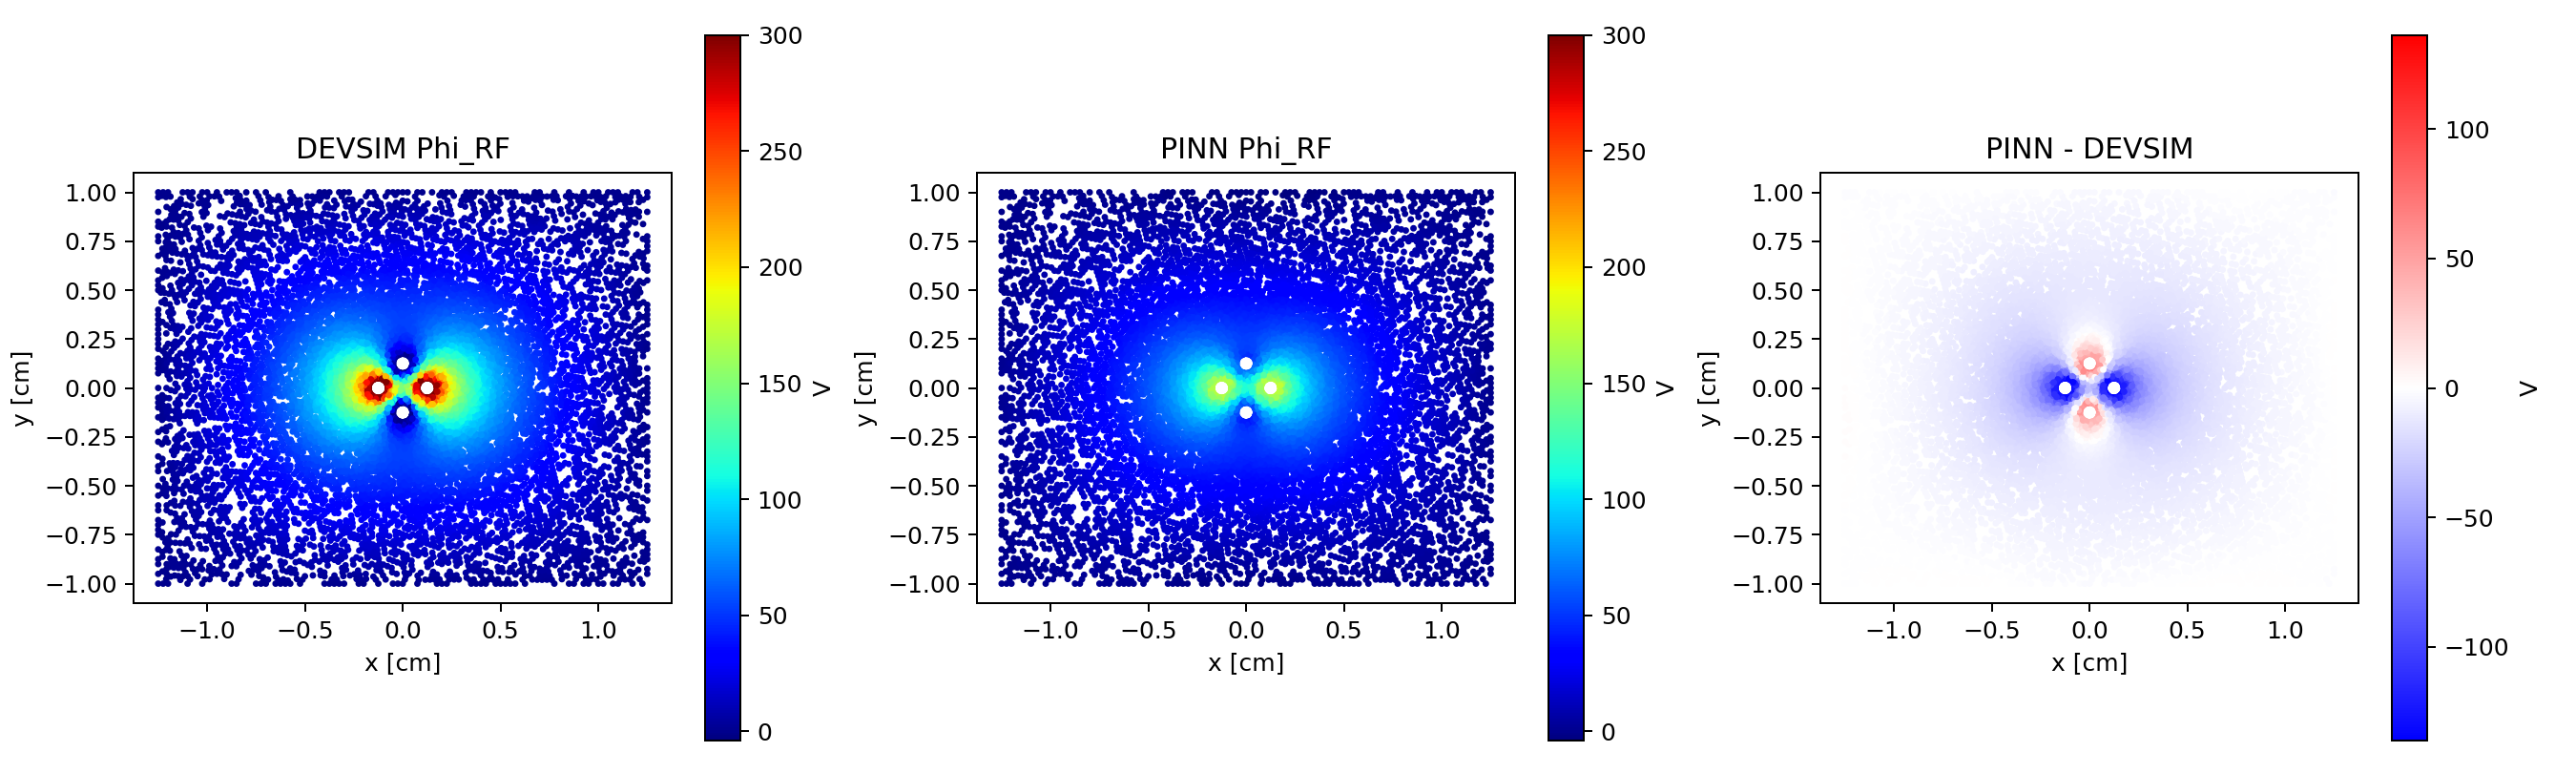
\includegraphics[width=\linewidth]{../runs/learning_rate_pinn_20260602_032454_lr_1e-4/comparison_phi_rf.png}
\end{column}
\begin{column}{0.49\textwidth}
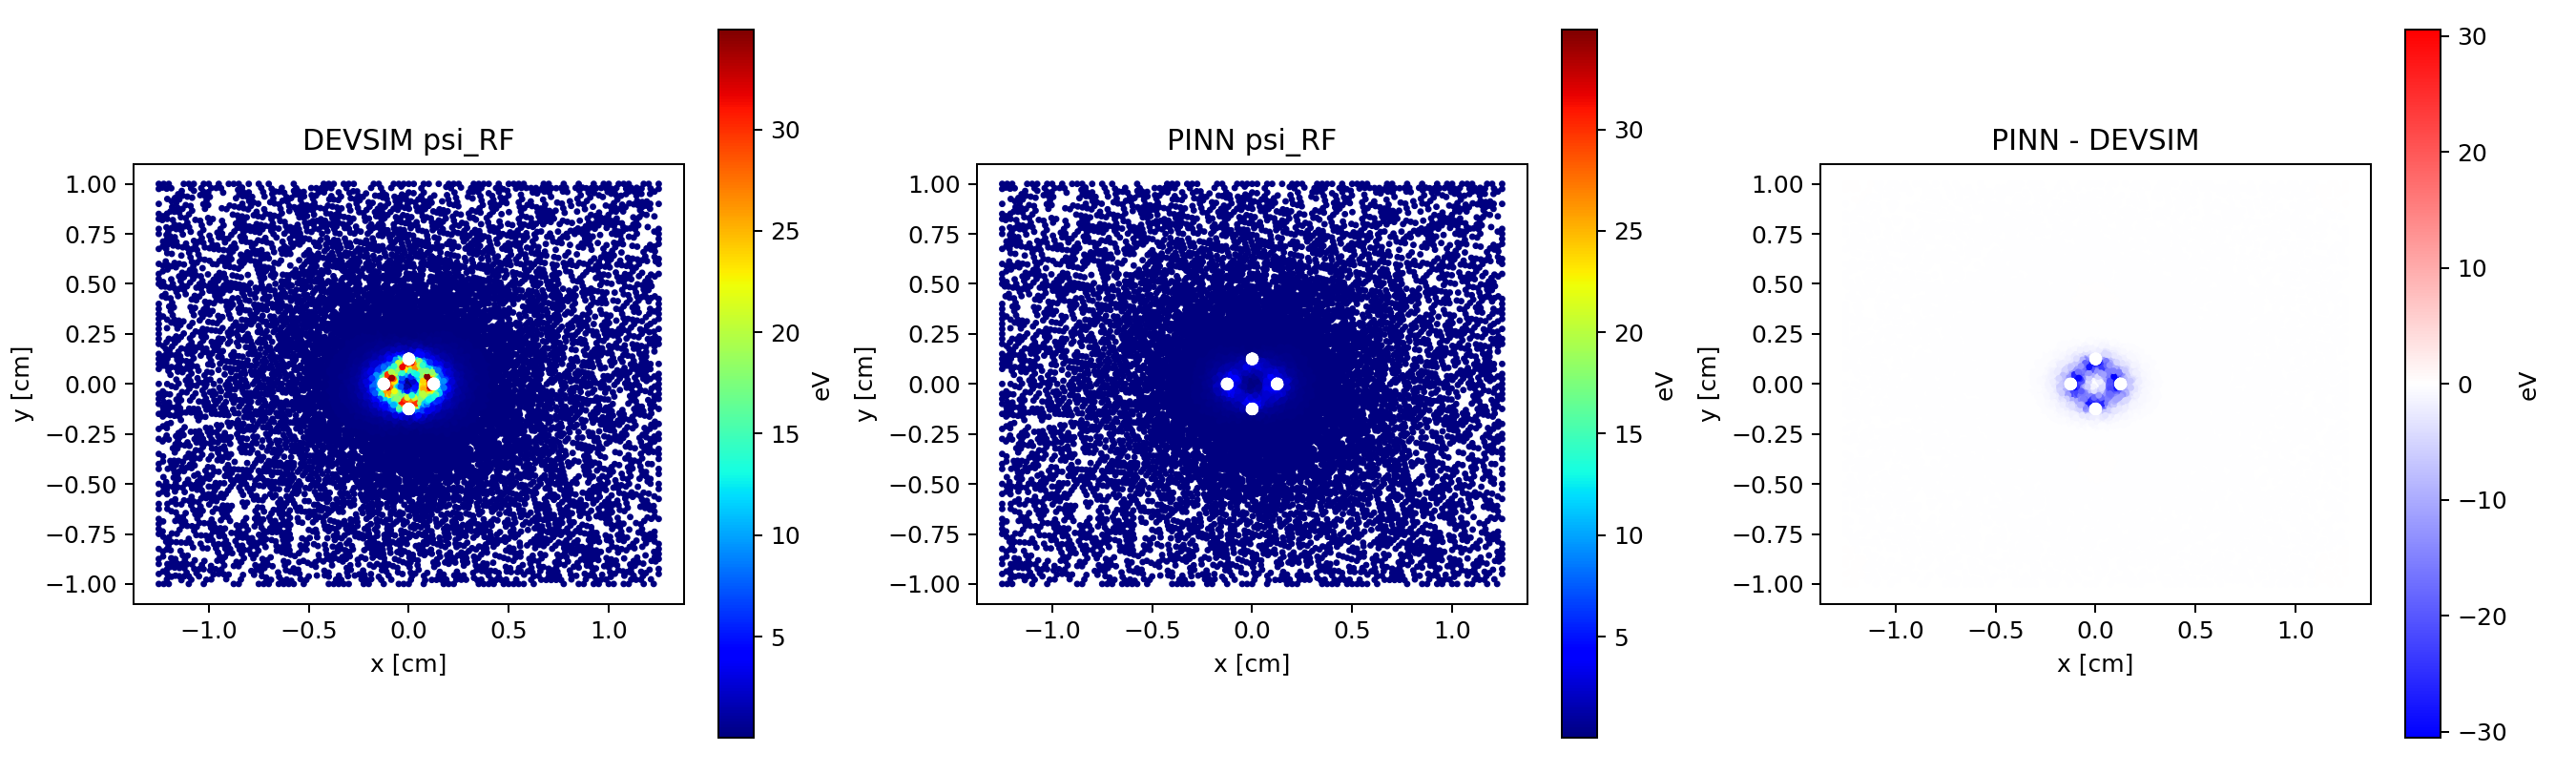
\includegraphics[width=\linewidth]{../runs/learning_rate_pinn_20260602_032454_lr_1e-4/comparison_psi_rf_eV.png}
\end{column}
\end{columns}
\vspace{0.08in}
\small Final normalized loss 0.251; Phi MSE 1.95e+03; Psi MSE 50.2.
\end{frame}

\begin{frame}[t]{lr\_3e-3}
\begin{columns}[T,onlytextwidth]
\begin{column}{0.49\textwidth}
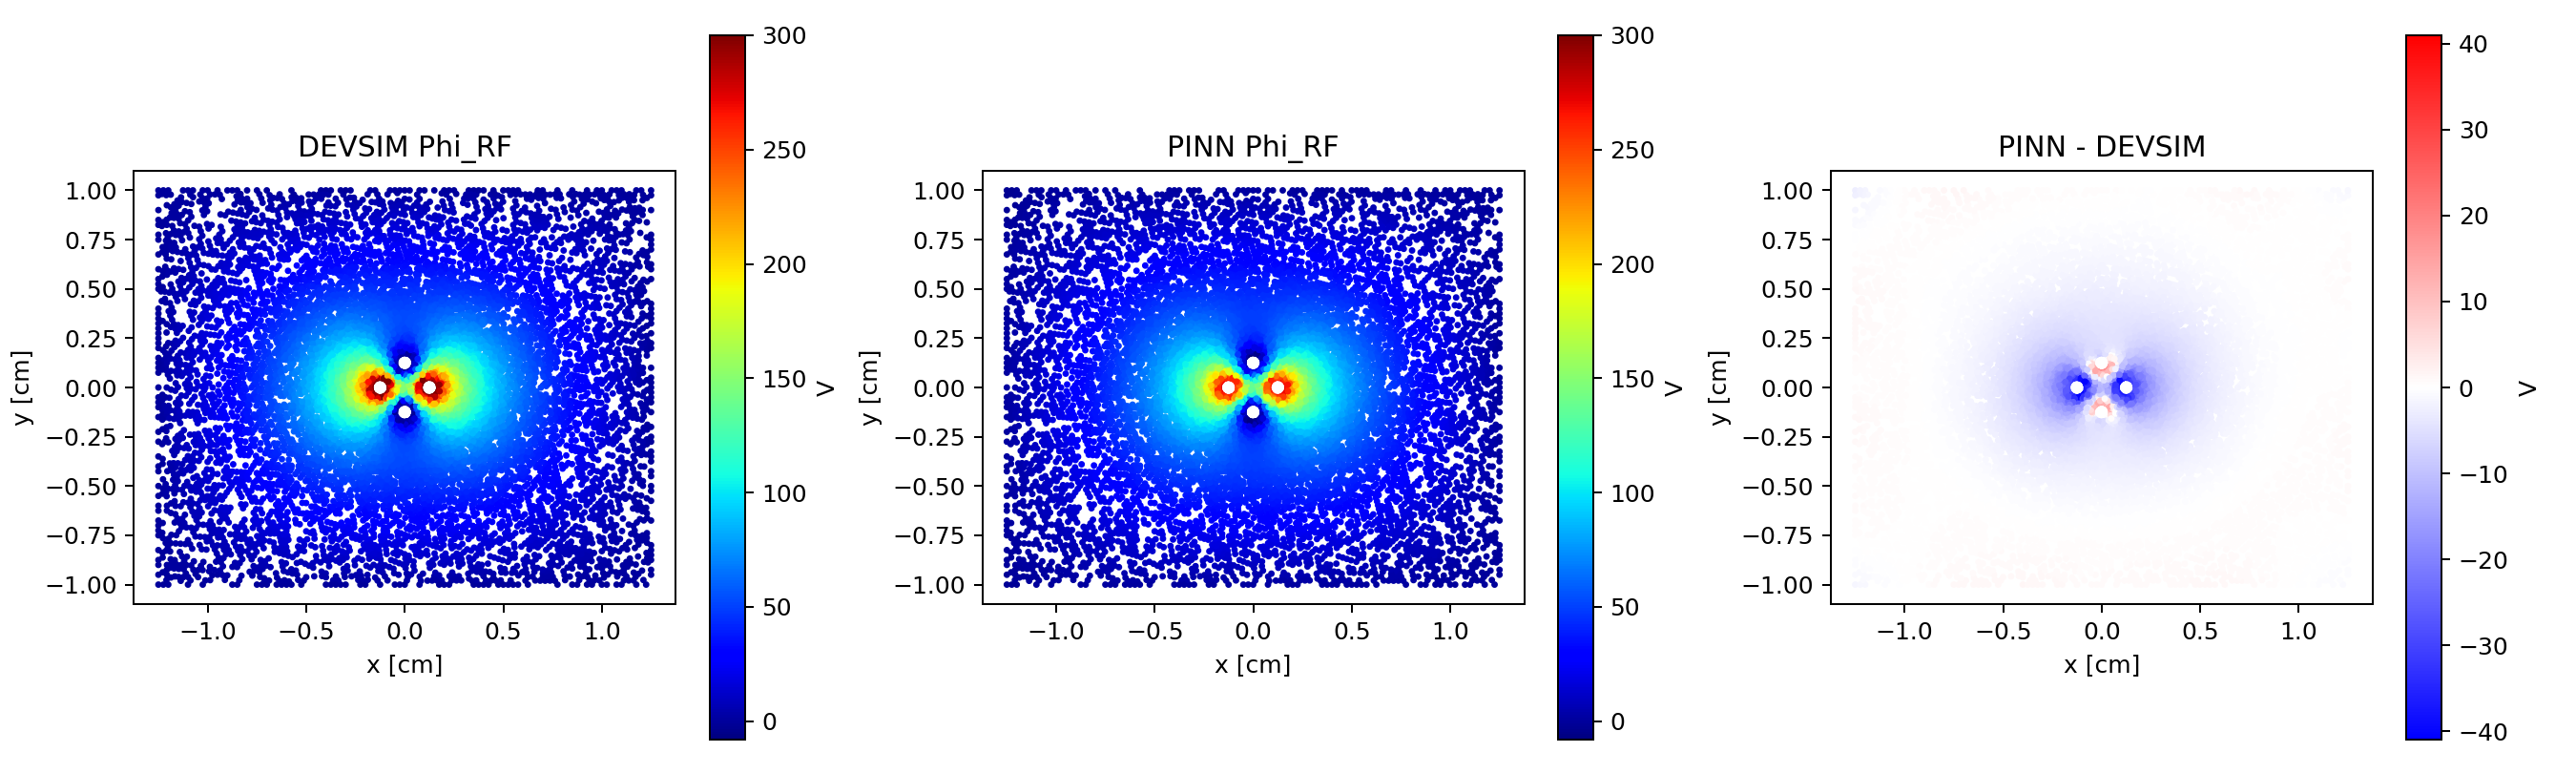
\includegraphics[width=\linewidth]{../runs/learning_rate_pinn_20260602_034642_lr_3e-3/comparison_phi_rf.png}
\end{column}
\begin{column}{0.49\textwidth}
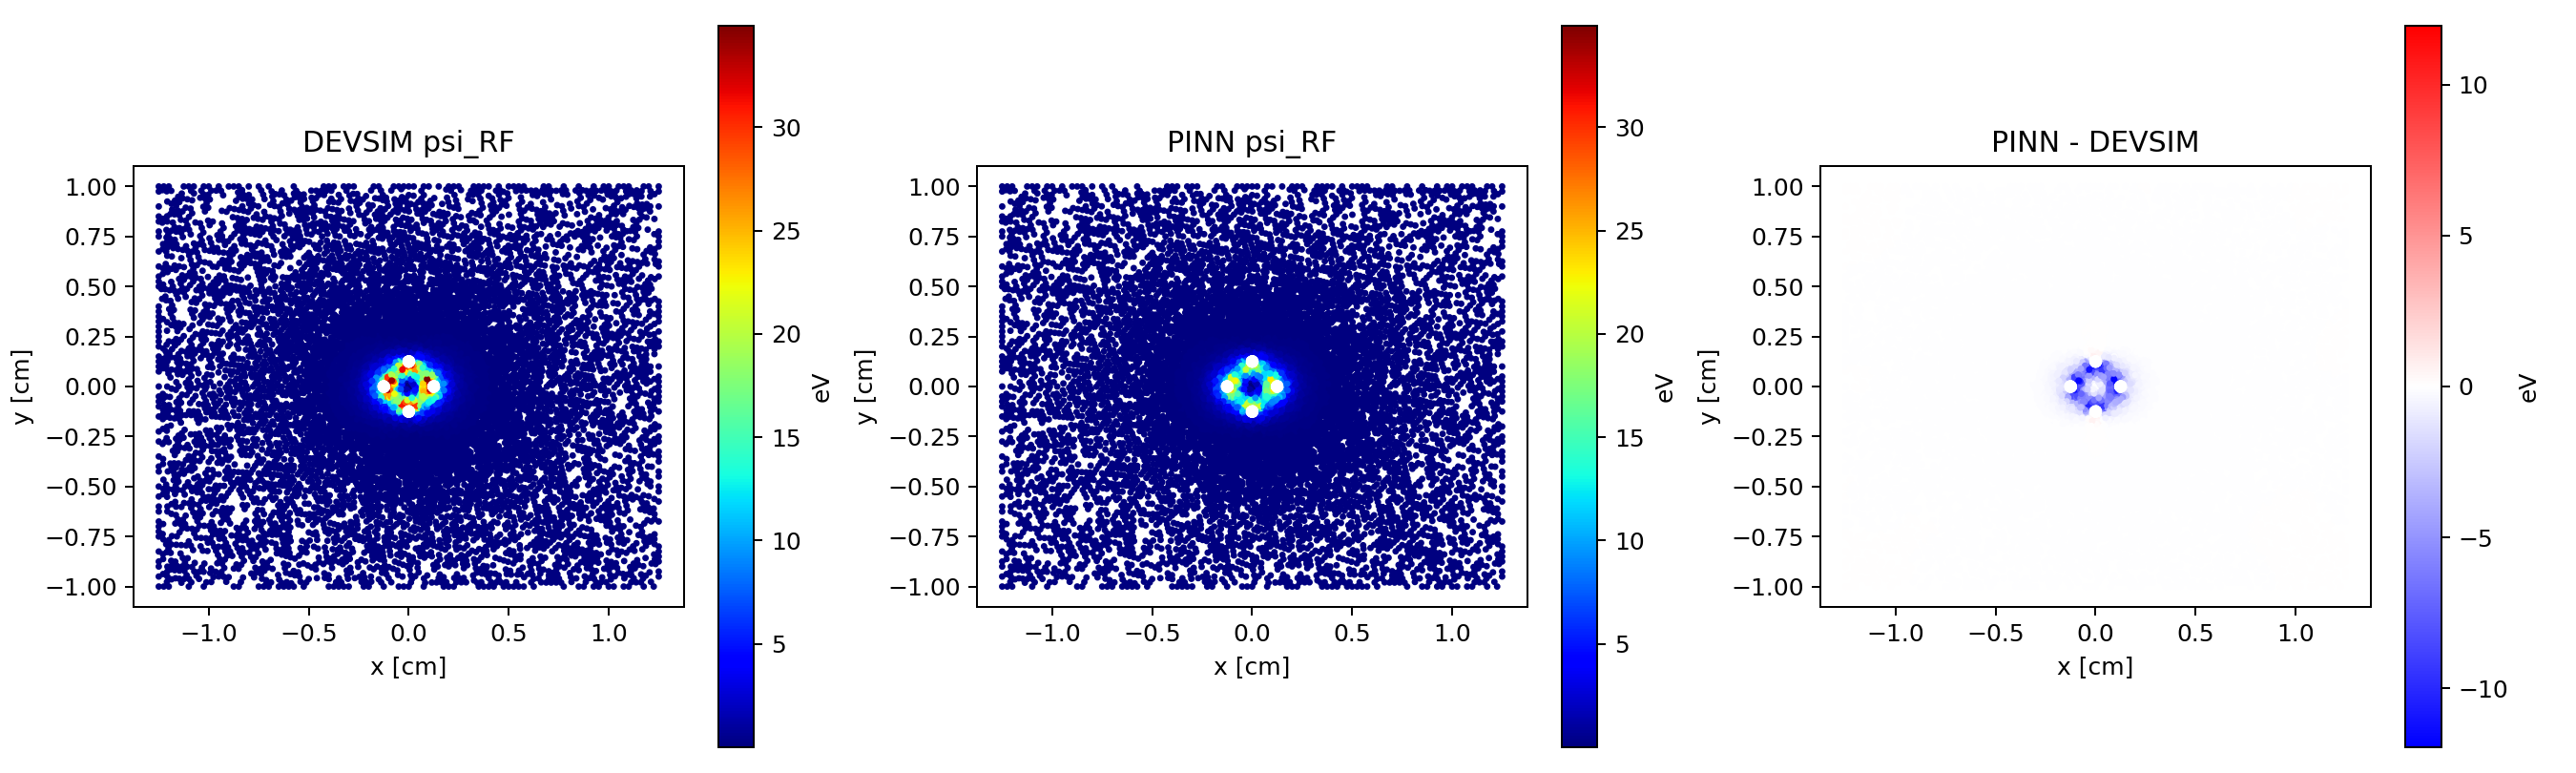
\includegraphics[width=\linewidth]{../runs/learning_rate_pinn_20260602_034642_lr_3e-3/comparison_psi_rf_eV.png}
\end{column}
\end{columns}
\vspace{0.08in}
\small Final normalized loss 0.493; Phi MSE 142; Psi MSE 6.57.
\end{frame}

\begin{frame}[t]{lr\_3e-4}
\begin{columns}[T,onlytextwidth]
\begin{column}{0.49\textwidth}
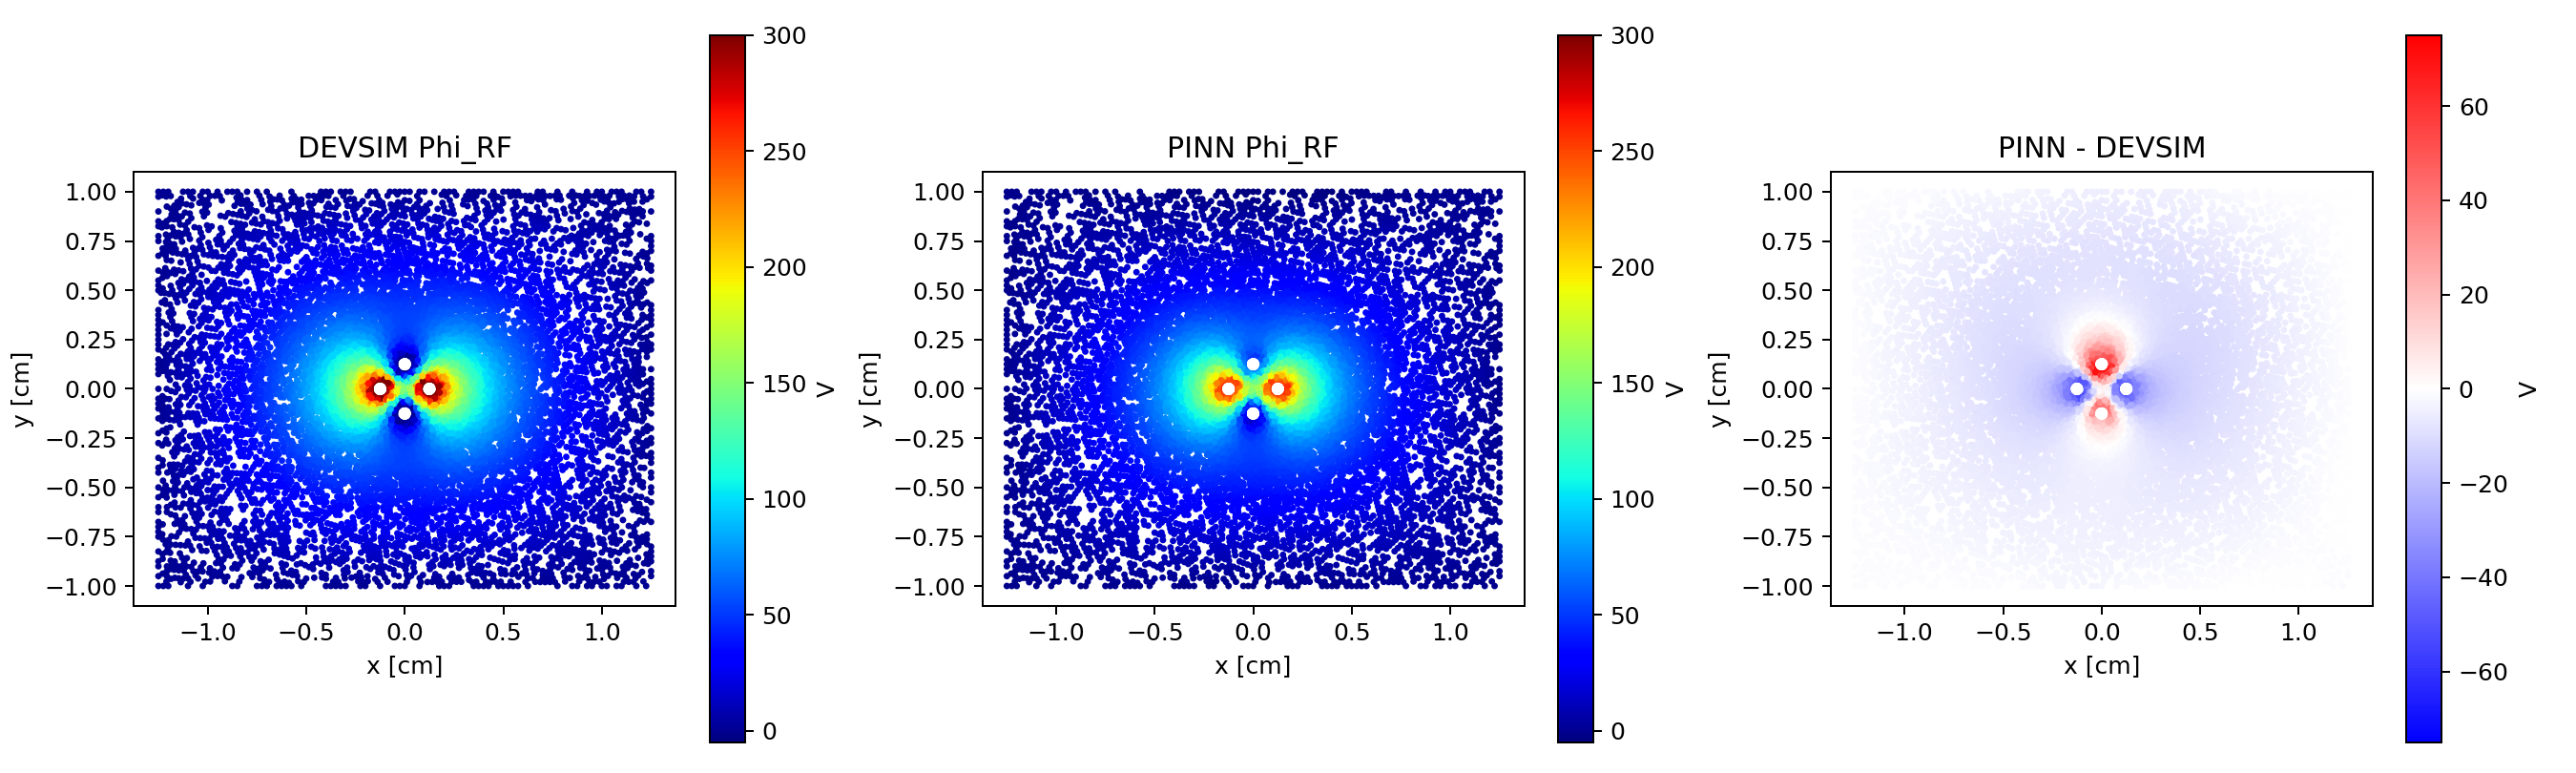
\includegraphics[width=\linewidth]{../runs/learning_rate_pinn_20260602_033556_lr_3e-4/comparison_phi_rf.png}
\end{column}
\begin{column}{0.49\textwidth}
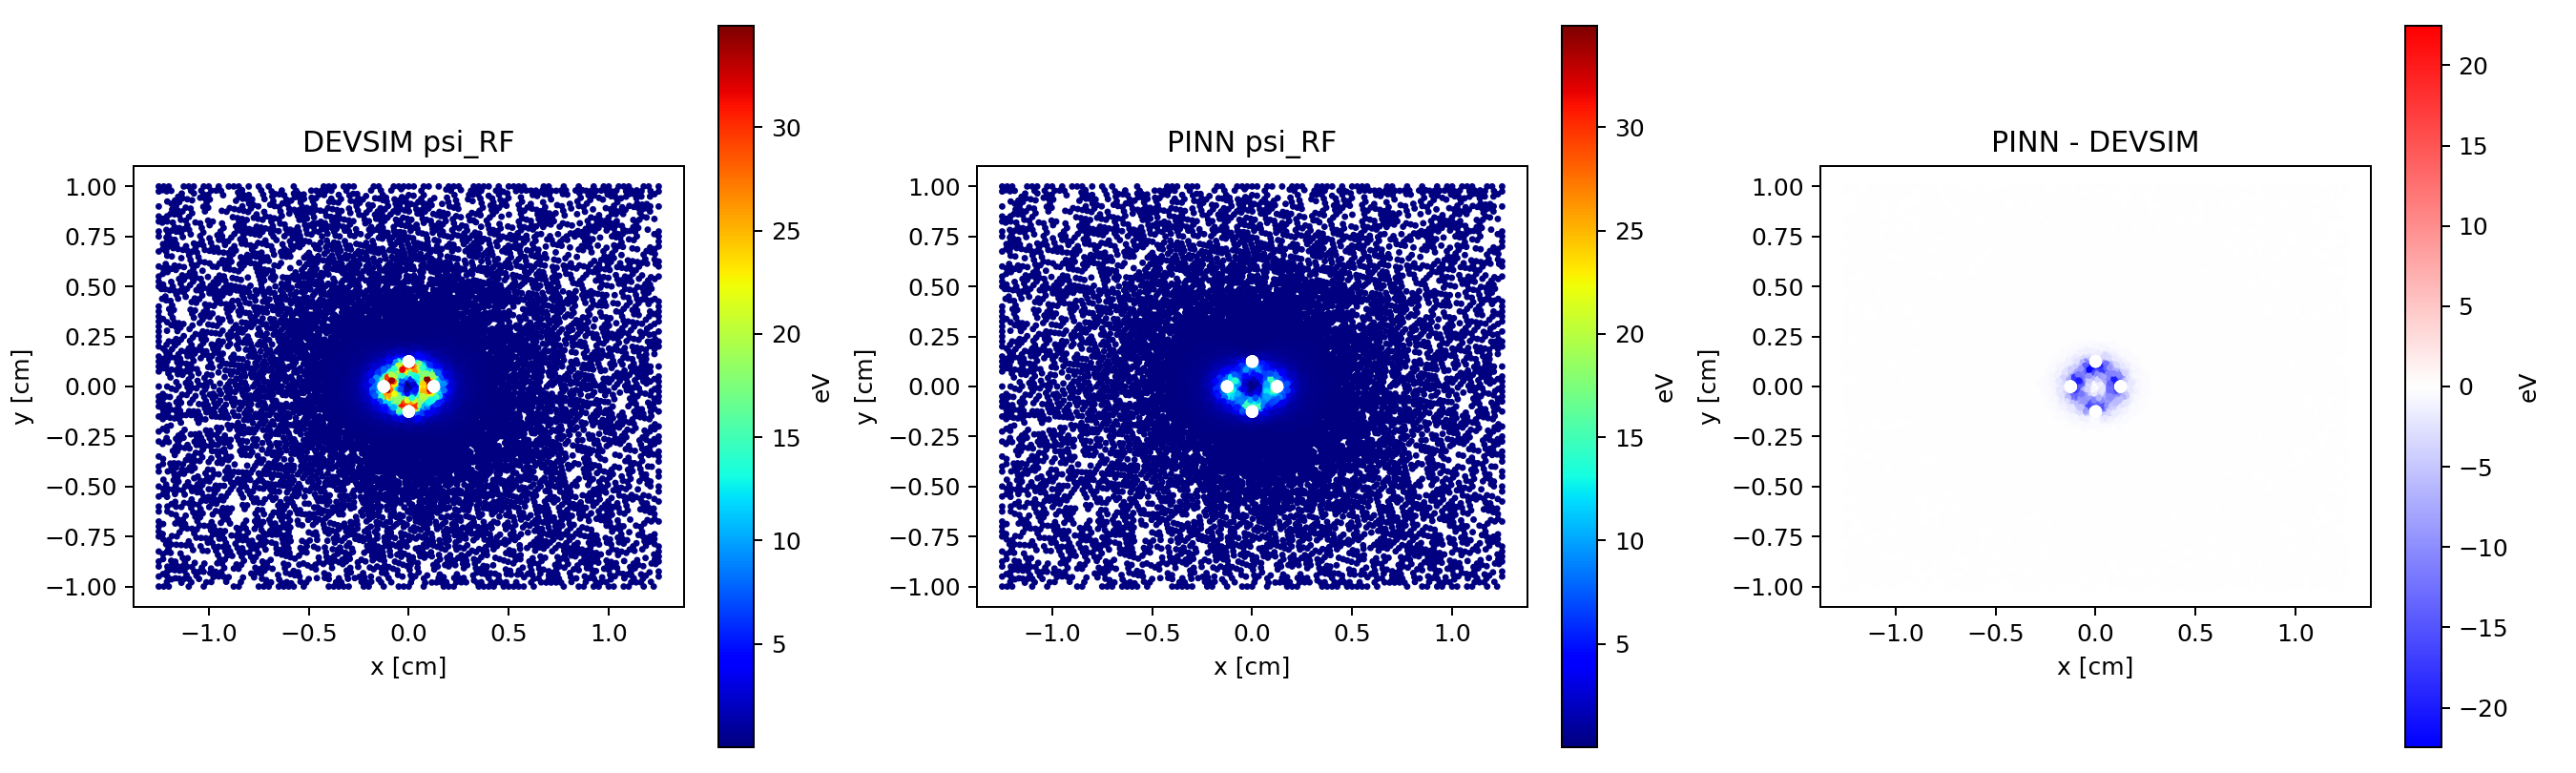
\includegraphics[width=\linewidth]{../runs/learning_rate_pinn_20260602_033556_lr_3e-4/comparison_psi_rf_eV.png}
\end{column}
\end{columns}
\vspace{0.08in}
\small Final normalized loss 0.149; Phi MSE 358; Psi MSE 21.3.
\end{frame}

\begin{frame}[t]{optimizer\_adamw}
\begin{columns}[T,onlytextwidth]
\begin{column}{0.49\textwidth}
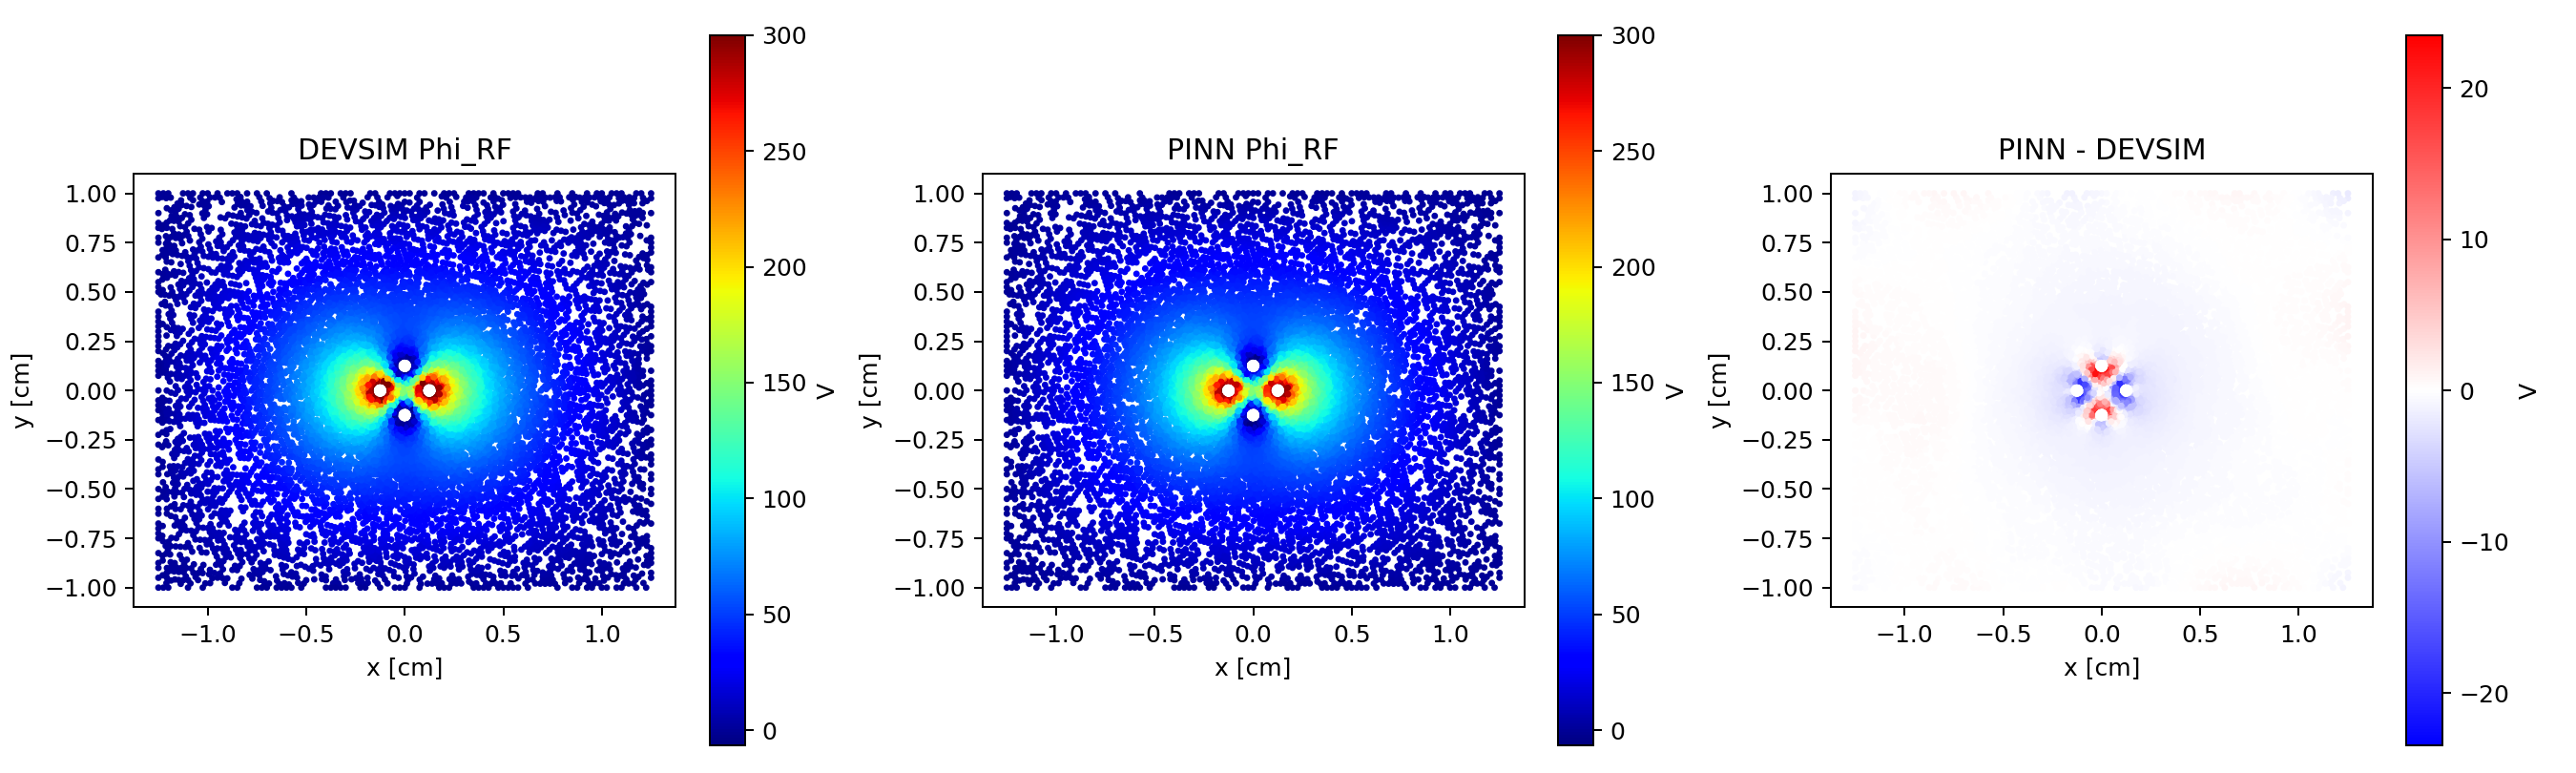
\includegraphics[width=\linewidth]{../runs/optimizer_pinn_20260602_025247_optimizer_adamw/comparison_phi_rf.png}
\end{column}
\begin{column}{0.49\textwidth}
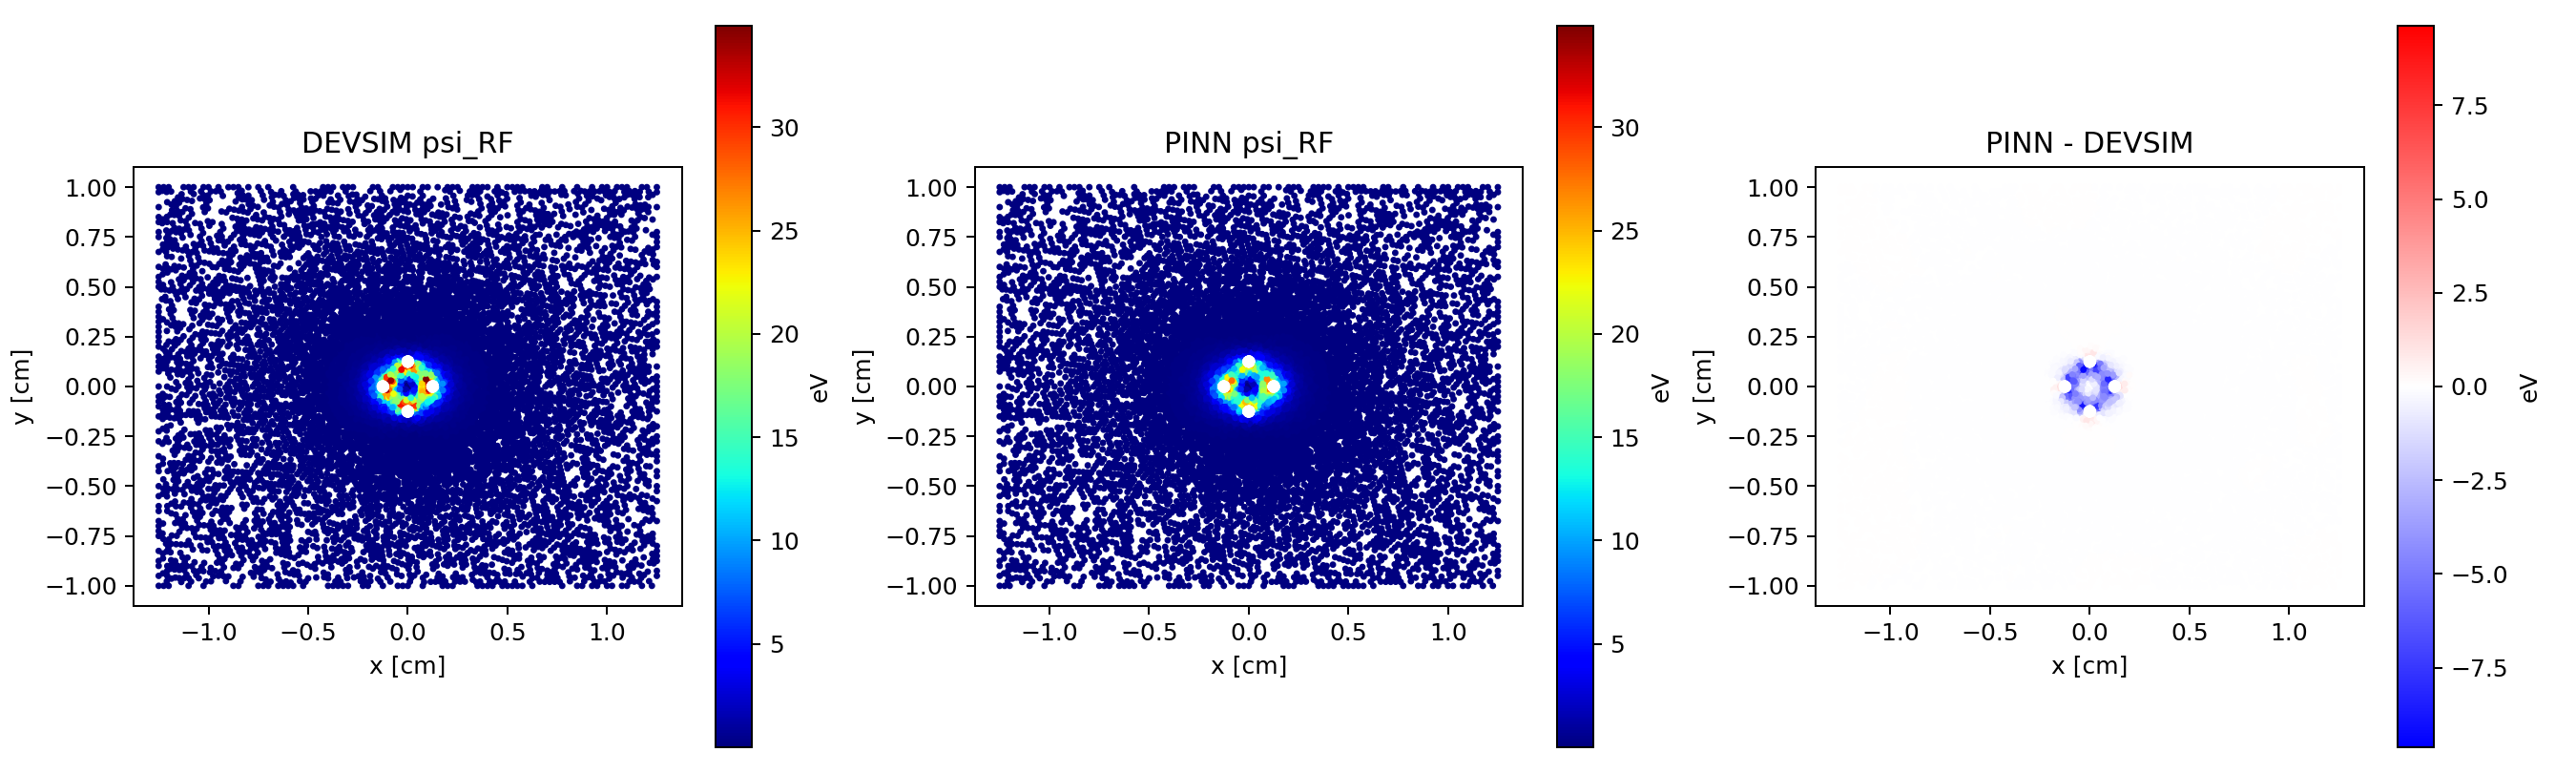
\includegraphics[width=\linewidth]{../runs/optimizer_pinn_20260602_025247_optimizer_adamw/comparison_psi_rf_eV.png}
\end{column}
\end{columns}
\vspace{0.08in}
\small Final normalized loss 0.0103; Phi MSE 21.9; Psi MSE 3.33.
\end{frame}

\begin{frame}[t]{optimizer\_rmsprop}
\begin{columns}[T,onlytextwidth]
\begin{column}{0.49\textwidth}
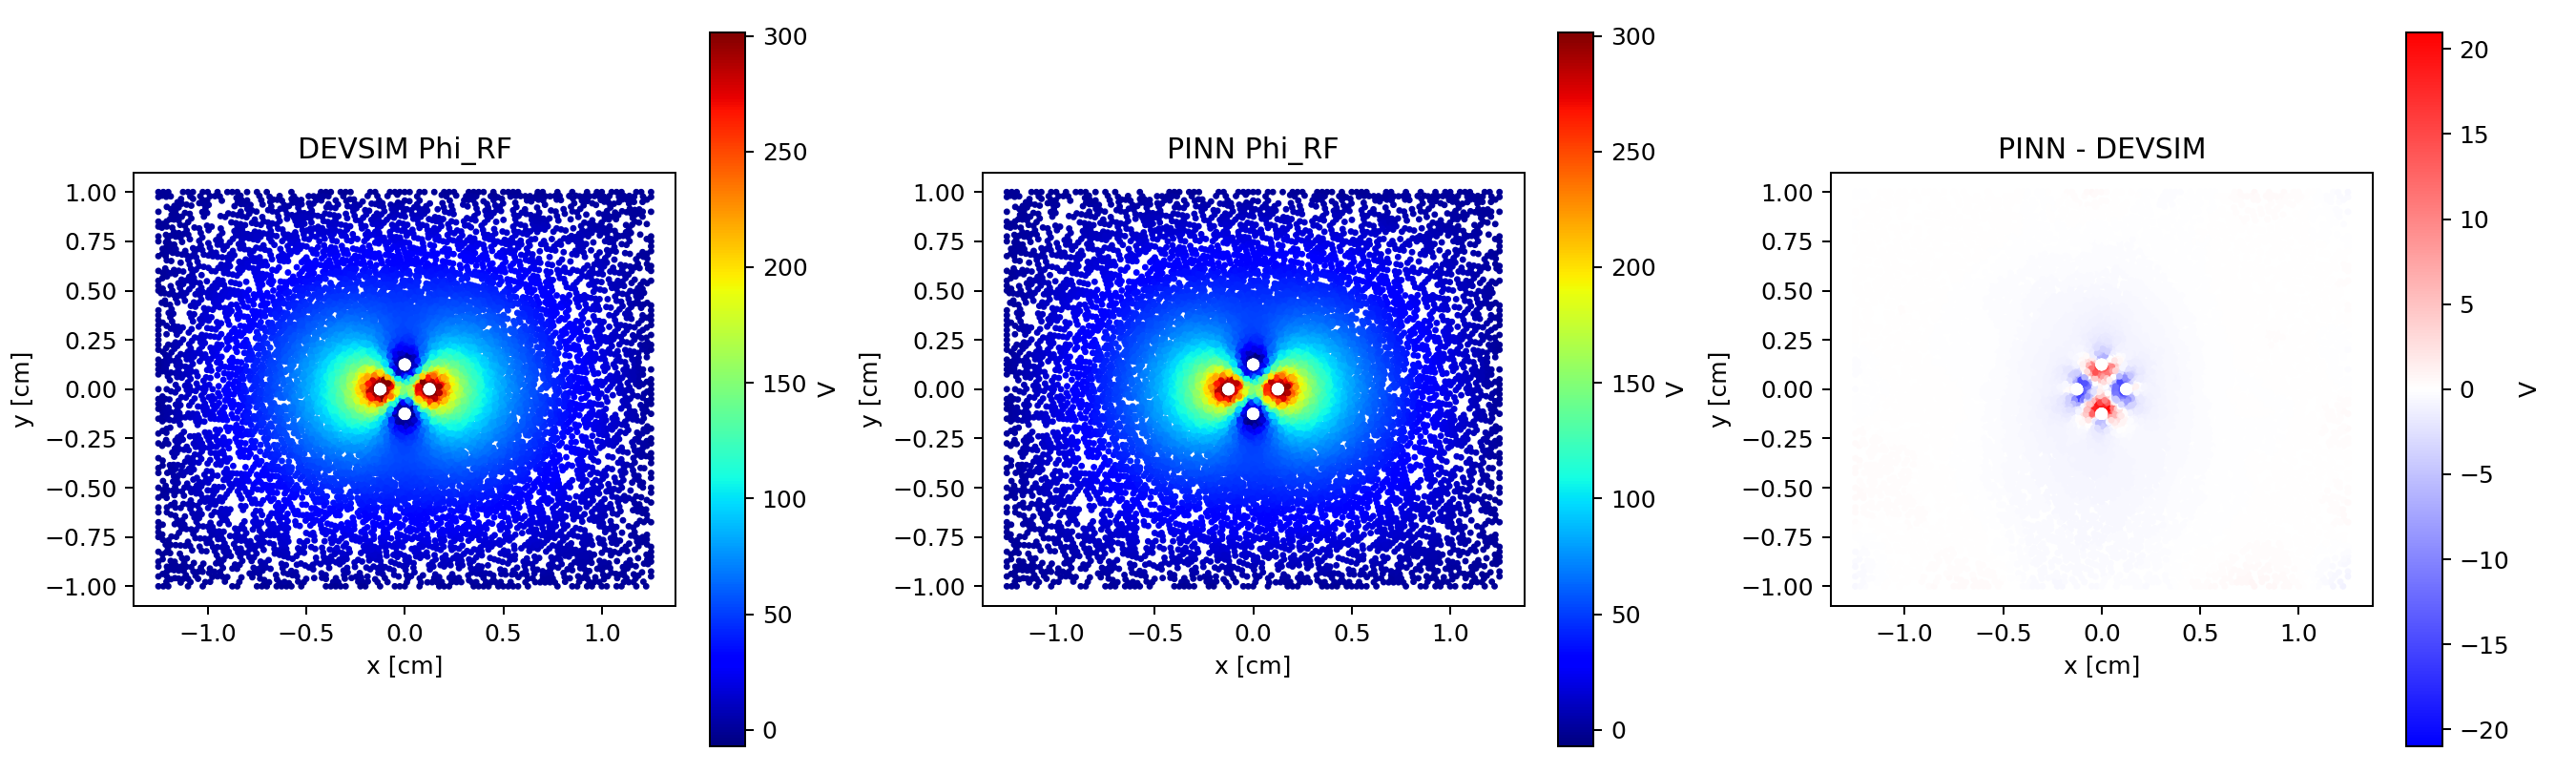
\includegraphics[width=\linewidth]{../runs/optimizer_pinn_20260602_030333_optimizer_rmsprop/comparison_phi_rf.png}
\end{column}
\begin{column}{0.49\textwidth}
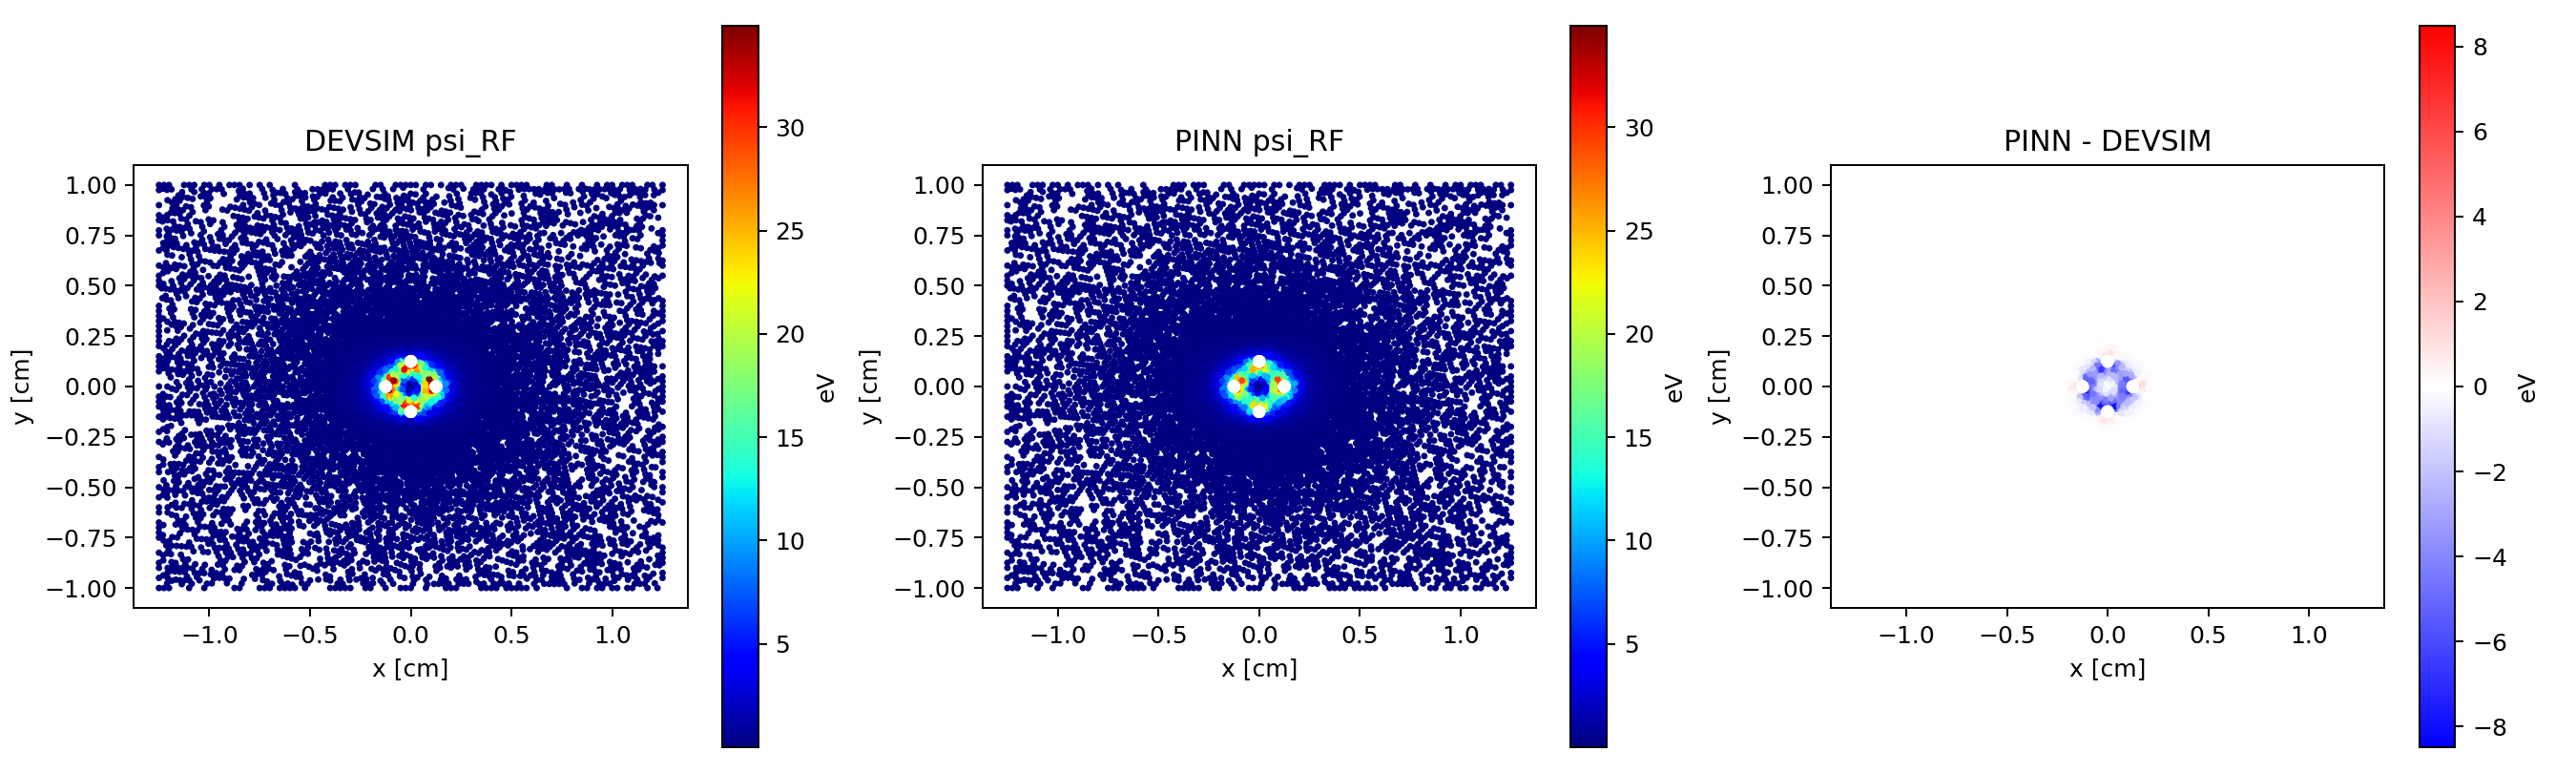
\includegraphics[width=\linewidth]{../runs/optimizer_pinn_20260602_030333_optimizer_rmsprop/comparison_psi_rf_eV.png}
\end{column}
\end{columns}
\vspace{0.08in}
\small Final normalized loss 0.0145; Phi MSE 14.5; Psi MSE 2.38.
\end{frame}

\begin{frame}[t]{optimizer\_sgd}
\begin{columns}[T,onlytextwidth]
\begin{column}{0.49\textwidth}
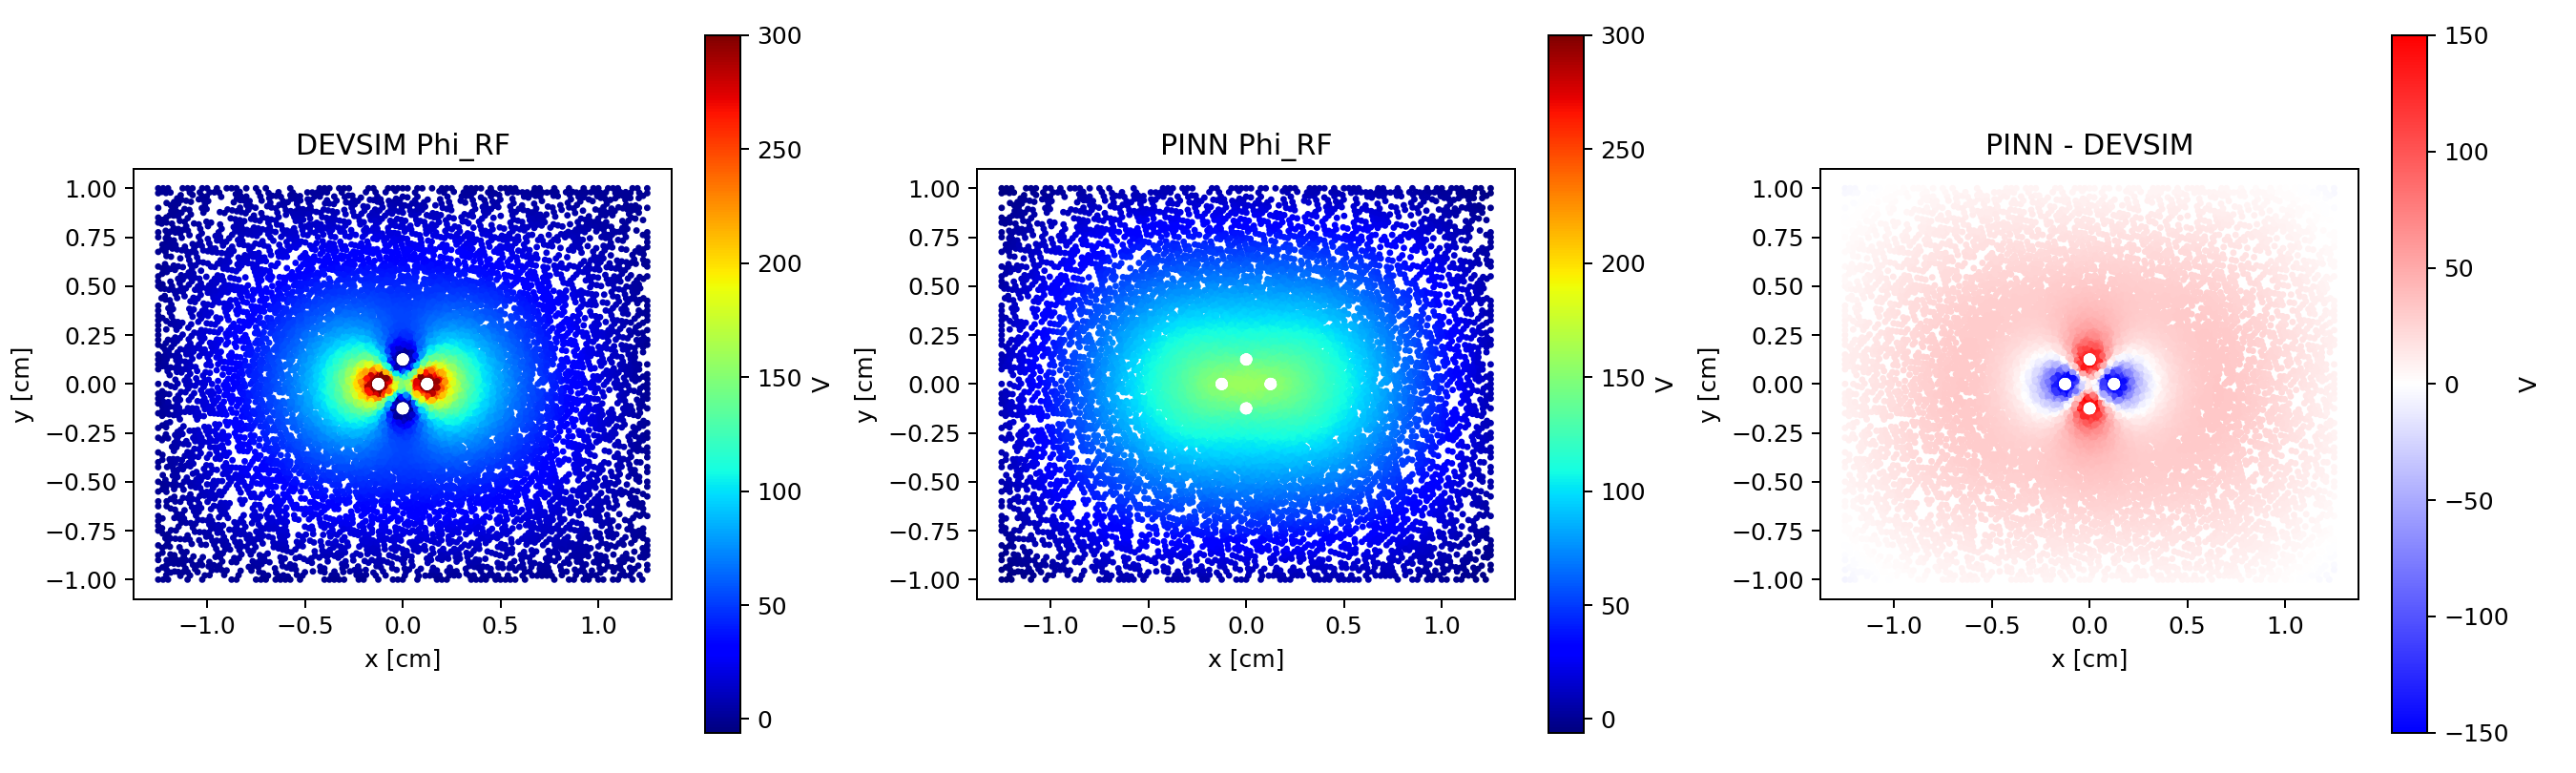
\includegraphics[width=\linewidth]{../runs/optimizer_pinn_20260602_031413_optimizer_sgd/comparison_phi_rf.png}
\end{column}
\begin{column}{0.49\textwidth}
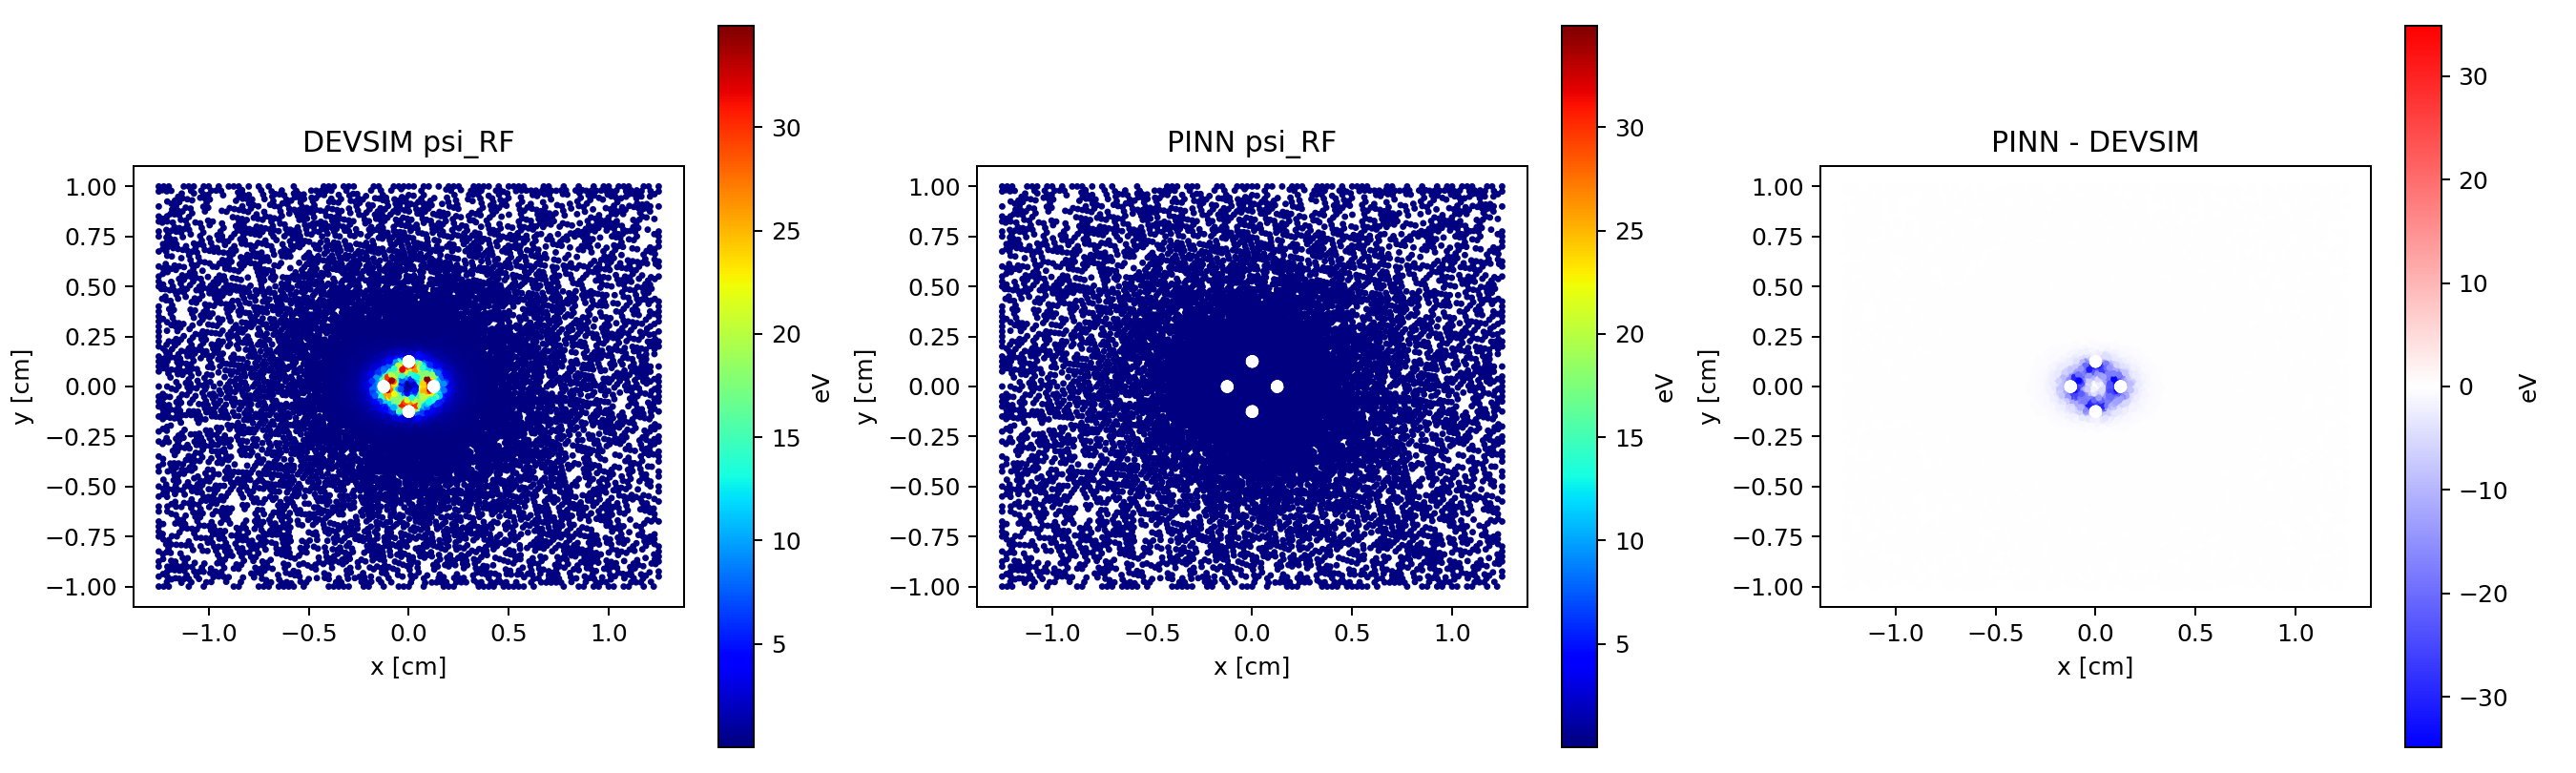
\includegraphics[width=\linewidth]{../runs/optimizer_pinn_20260602_031413_optimizer_sgd/comparison_psi_rf_eV.png}
\end{column}
\end{columns}
\vspace{0.08in}
\small SGD plateaued; comparison confirms poor field accuracy for this training budget.
\end{frame}

\begin{frame}[t]{width\_256}
\begin{columns}[T,onlytextwidth]
\begin{column}{0.49\textwidth}
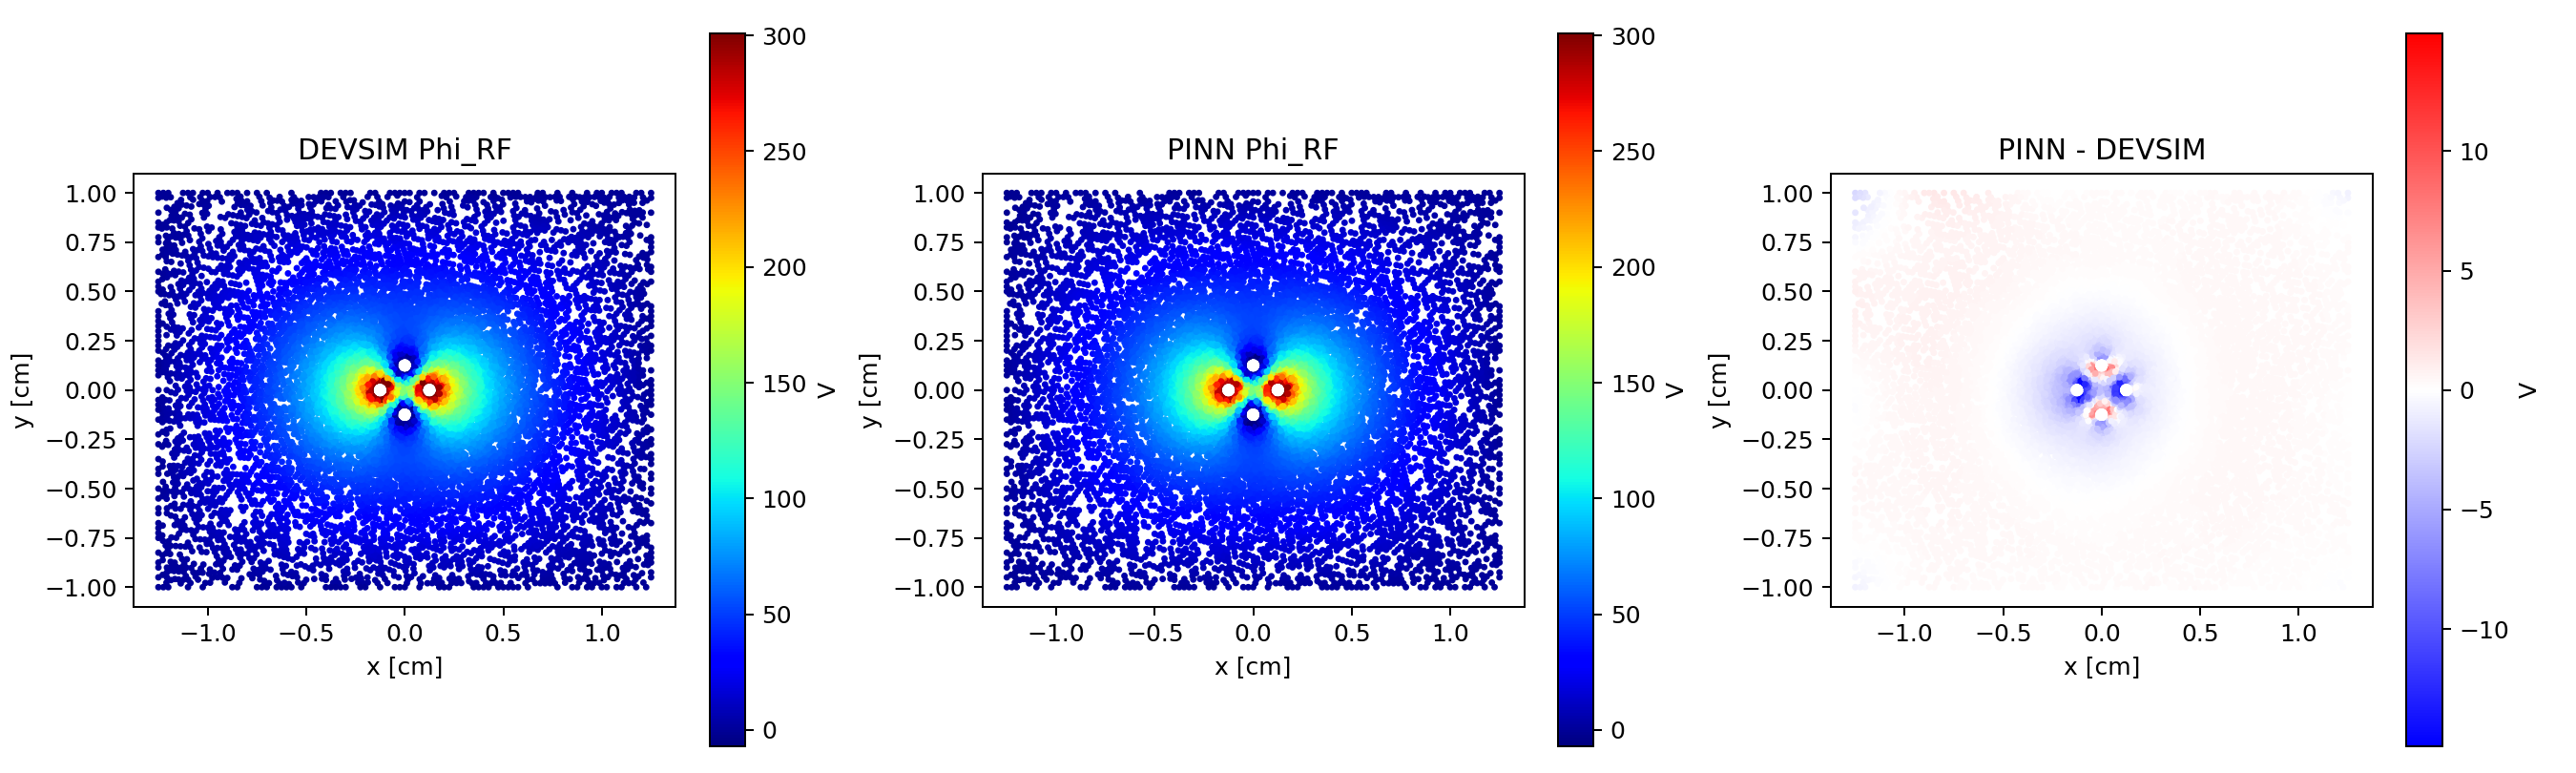
\includegraphics[width=\linewidth]{../runs/width_pinn_20260602_002701_width_256/comparison_phi_rf.png}
\end{column}
\begin{column}{0.49\textwidth}
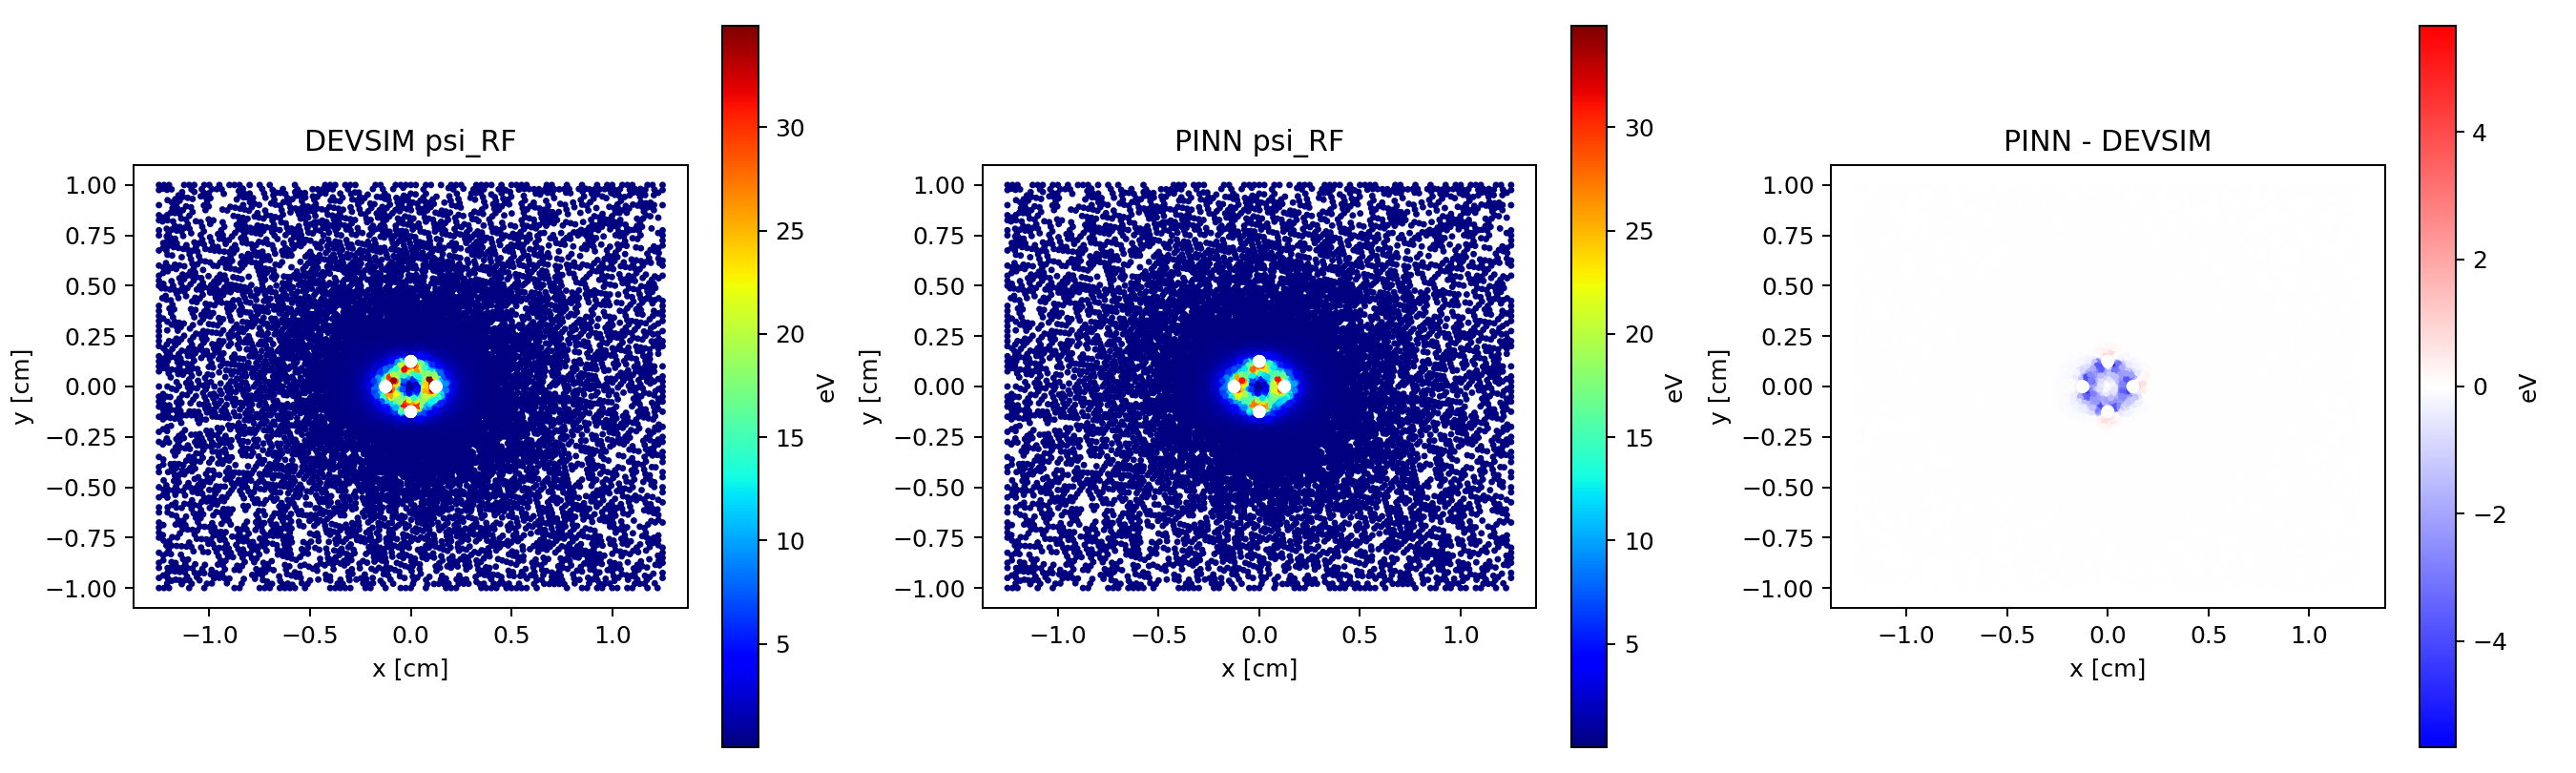
\includegraphics[width=\linewidth]{../runs/width_pinn_20260602_002701_width_256/comparison_psi_rf_eV.png}
\end{column}
\end{columns}
\vspace{0.08in}
\small Best width result; wider representation improved physical field shape.
\end{frame}

\begin{frame}[t]{width\_32}
\begin{columns}[T,onlytextwidth]
\begin{column}{0.49\textwidth}
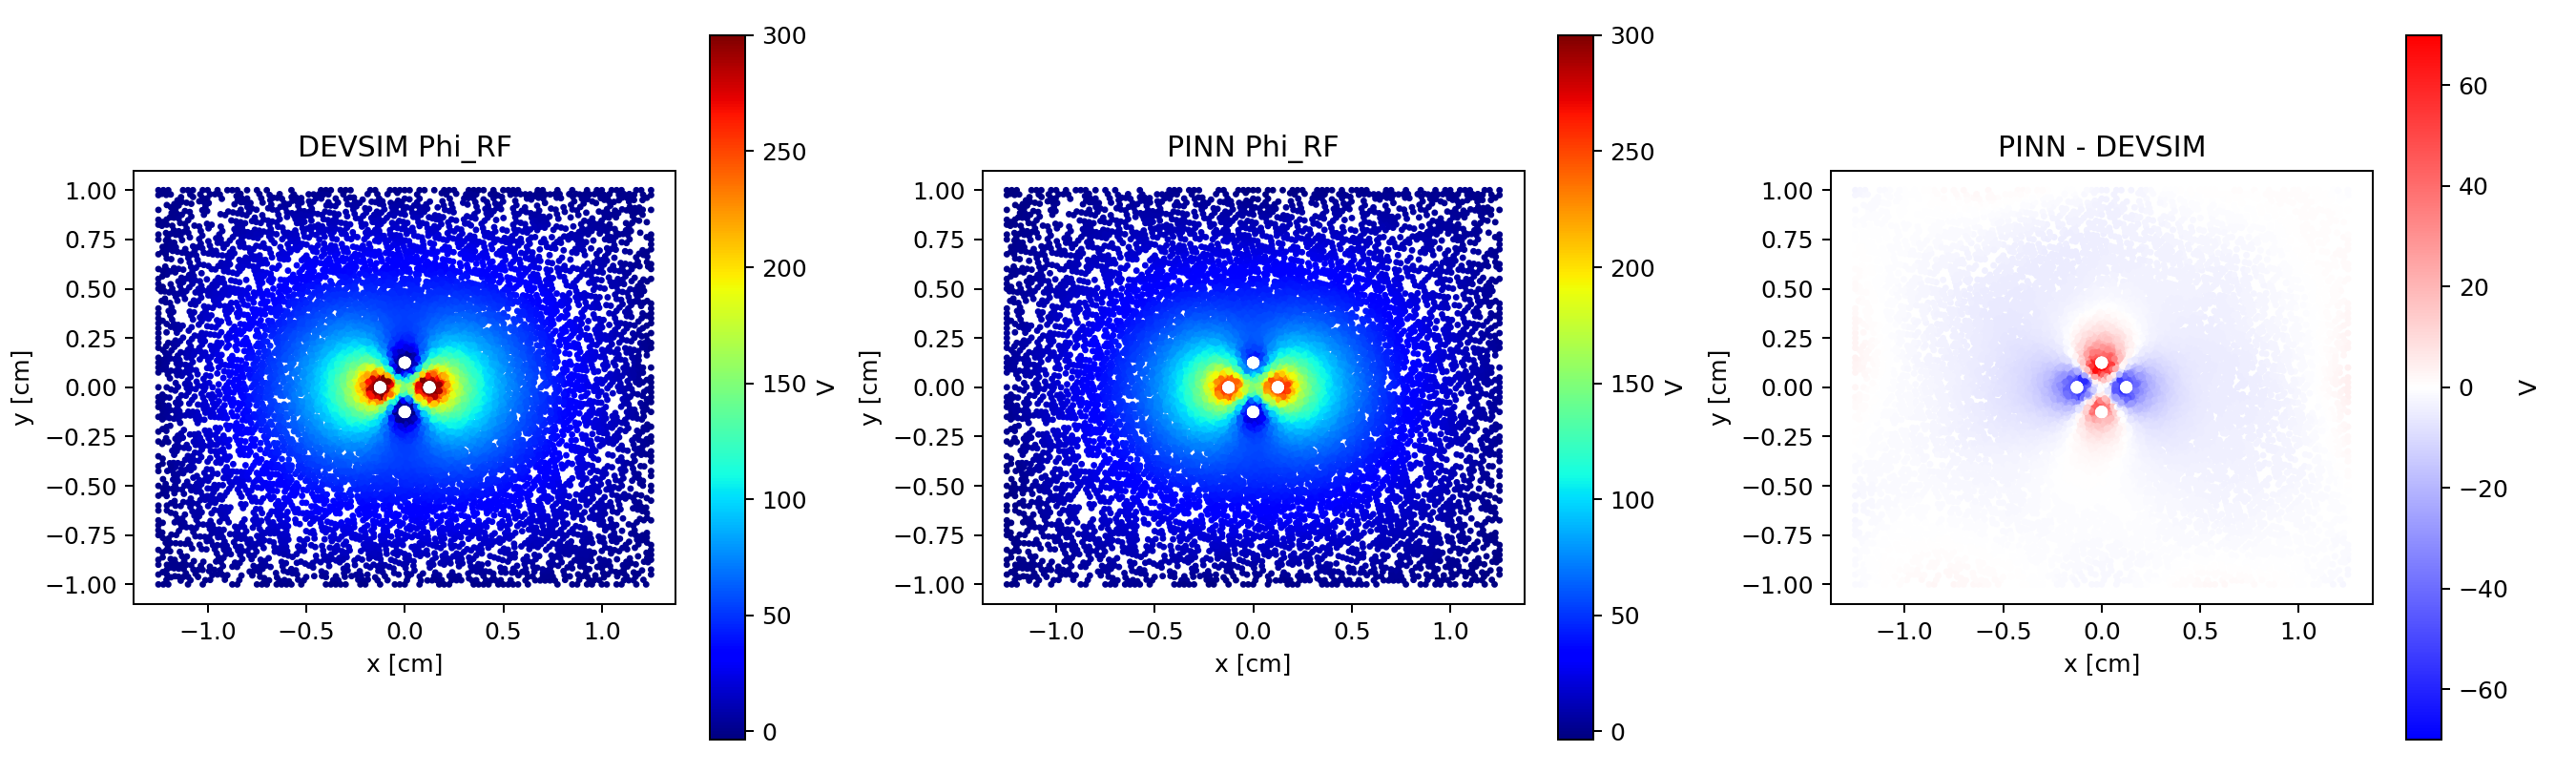
\includegraphics[width=\linewidth]{../runs/width_pinn_20260602_001737_width_32/comparison_phi_rf.png}
\end{column}
\begin{column}{0.49\textwidth}
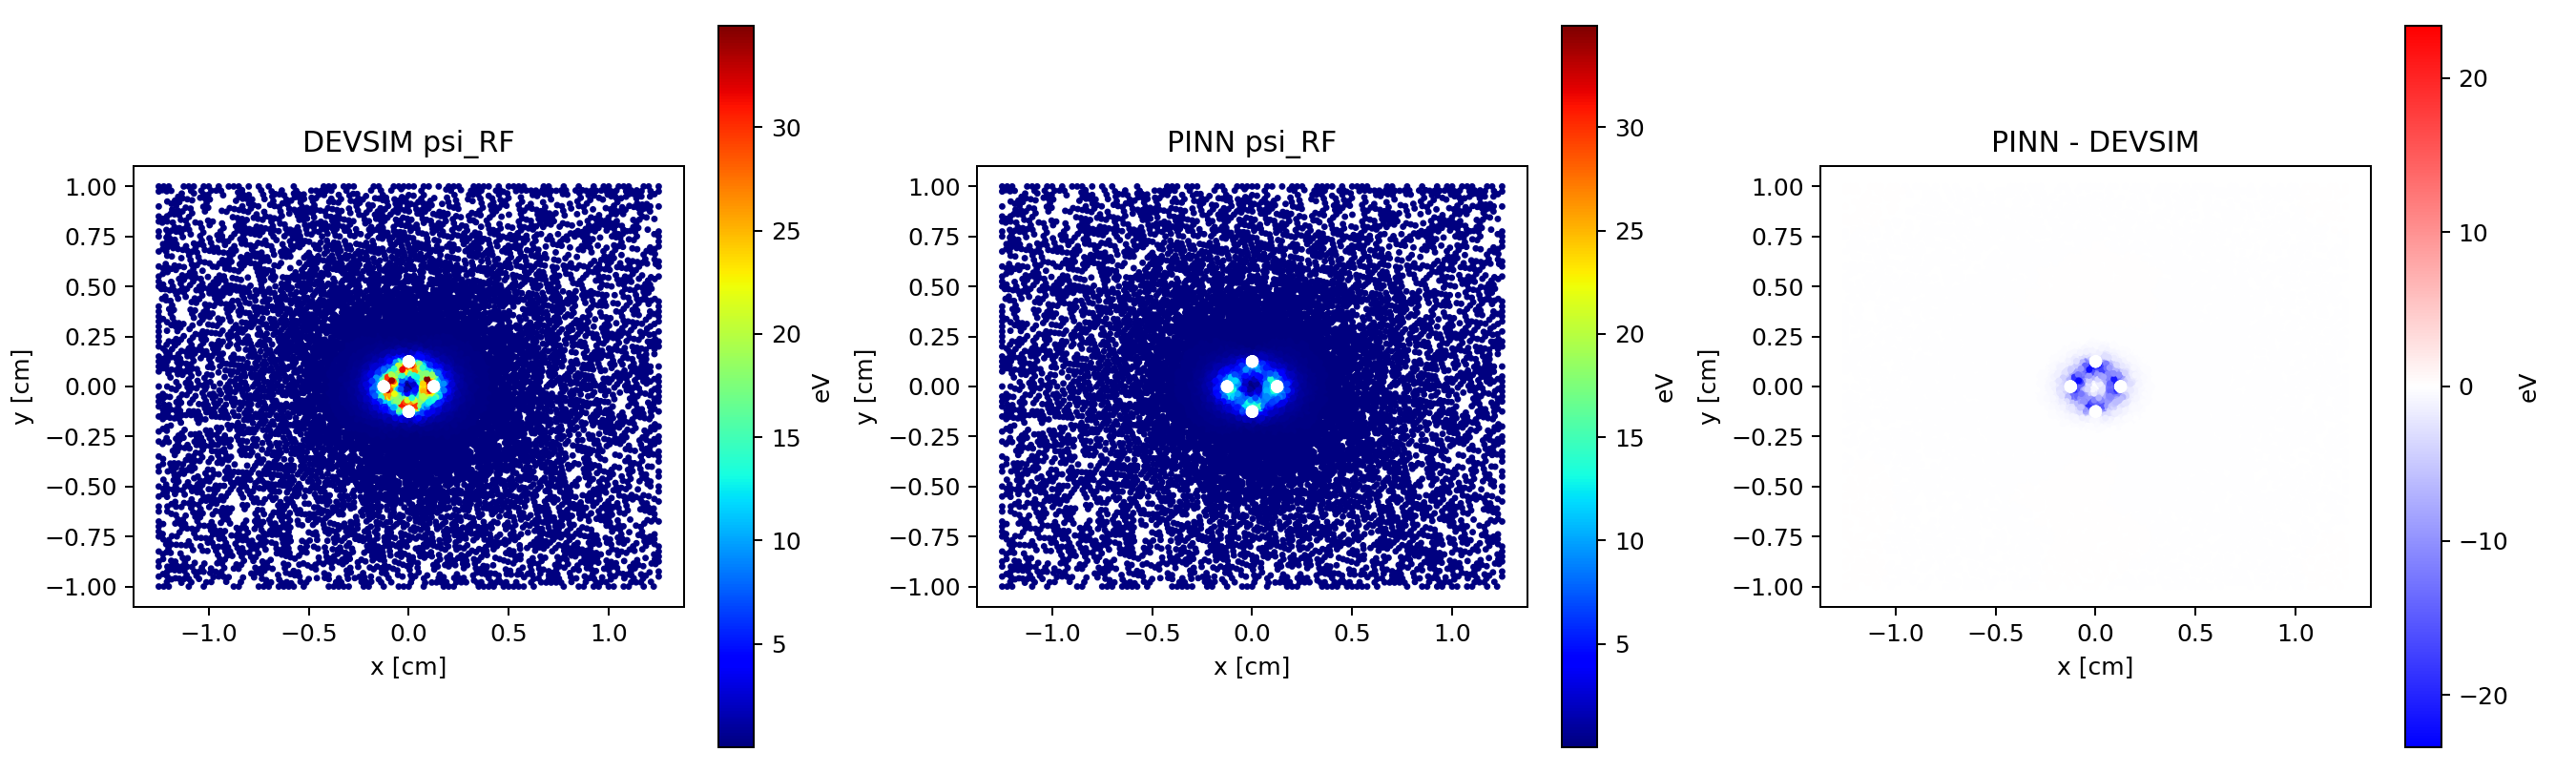
\includegraphics[width=\linewidth]{../runs/width_pinn_20260602_001737_width_32/comparison_psi_rf_eV.png}
\end{column}
\end{columns}
\vspace{0.08in}
\small Final normalized loss 0.0767; Phi MSE 334; Psi MSE 22.5.
\end{frame}

\begin{frame}[t]{width\_64}
\begin{columns}[T,onlytextwidth]
\begin{column}{0.49\textwidth}
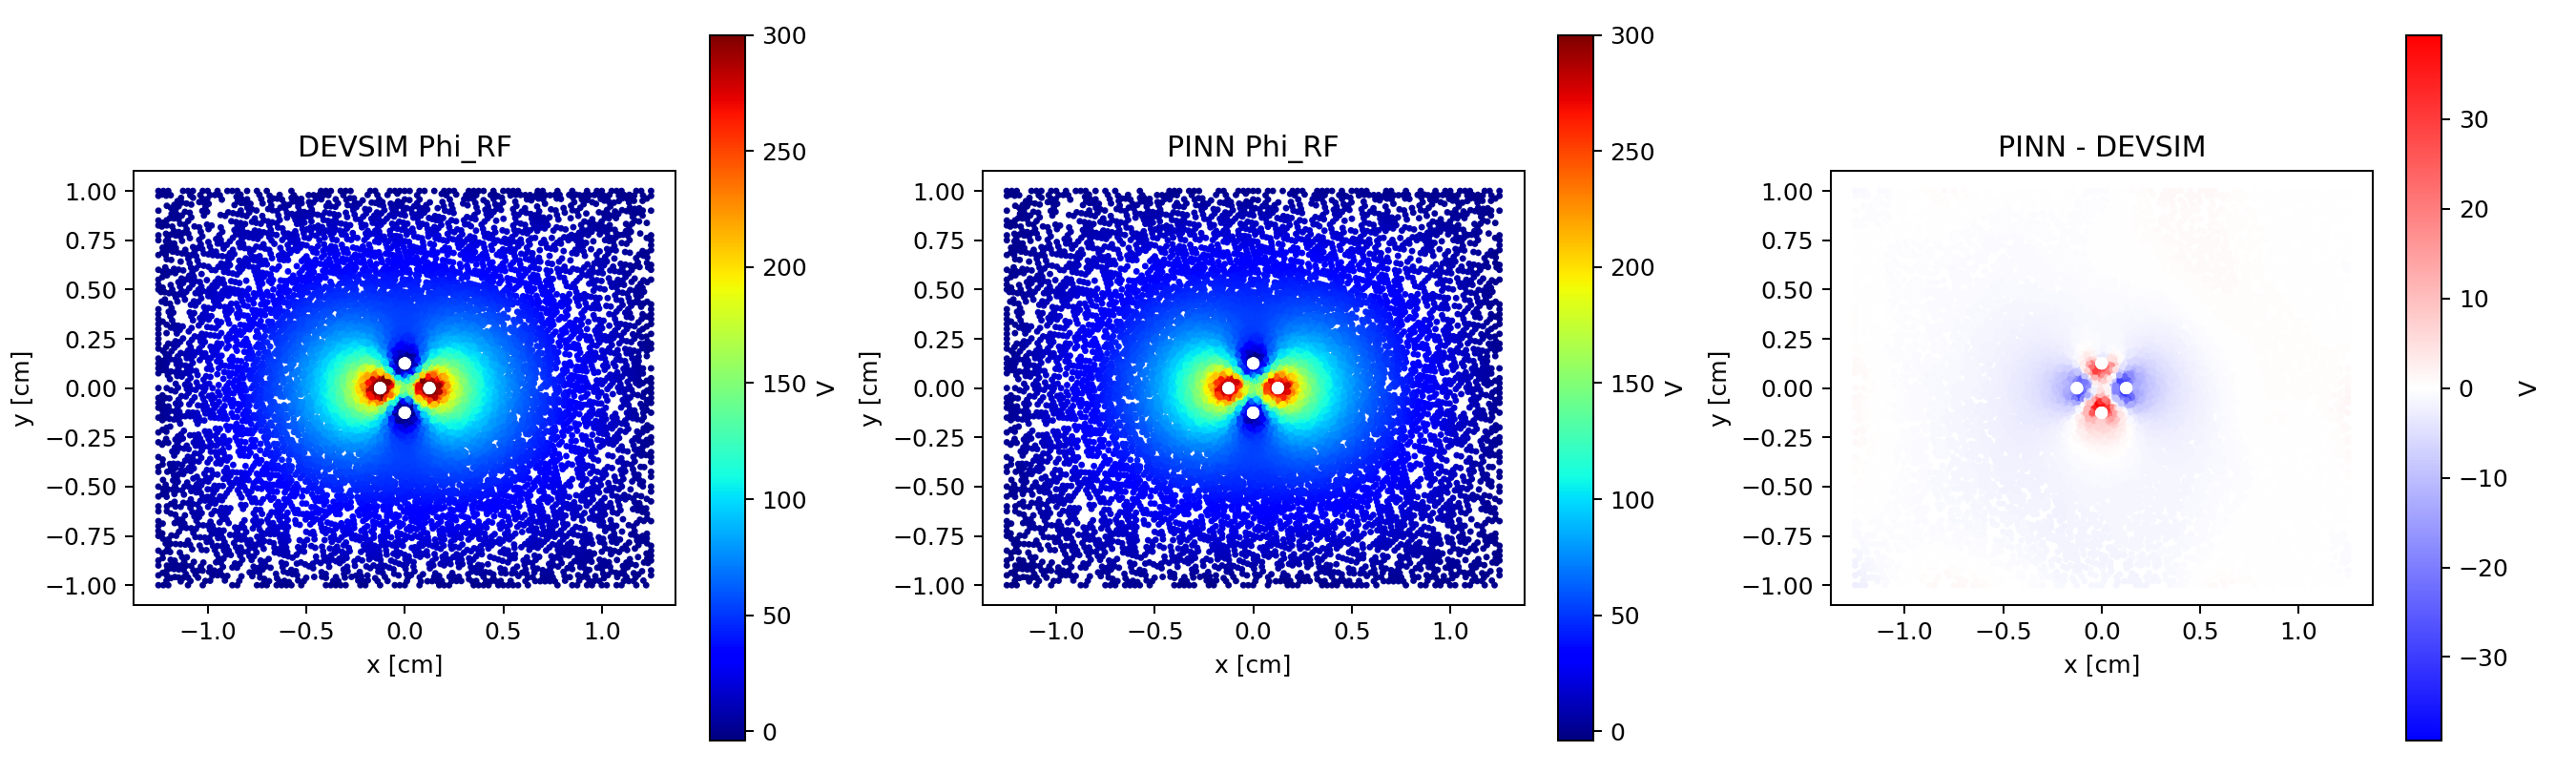
\includegraphics[width=\linewidth]{../runs/width_pinn_20260602_002108_width_64/comparison_phi_rf.png}
\end{column}
\begin{column}{0.49\textwidth}
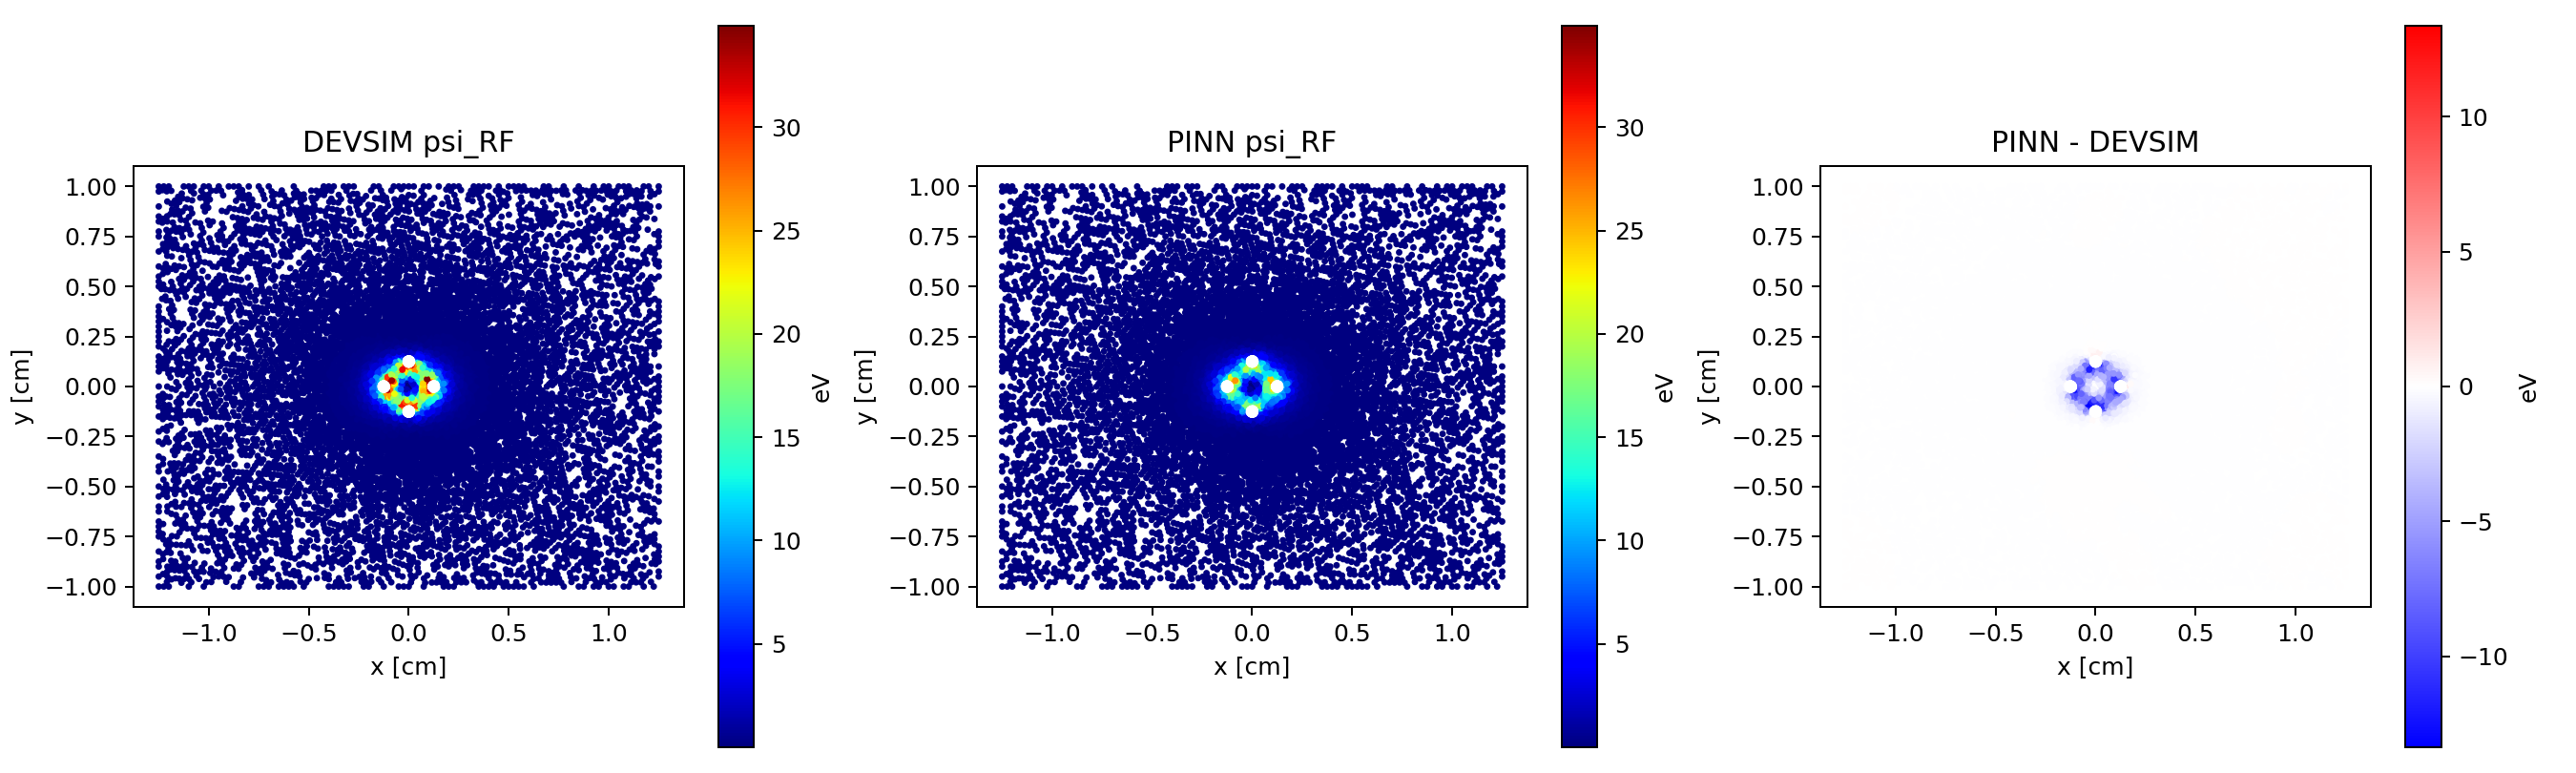
\includegraphics[width=\linewidth]{../runs/width_pinn_20260602_002108_width_64/comparison_psi_rf_eV.png}
\end{column}
\end{columns}
\vspace{0.08in}
\small Final normalized loss 0.02; Phi MSE 69.2; Psi MSE 7.33.
\end{frame}

\begin{frame}[t]{Discussion Summary}
\scriptsize
\setlength{\parindent}{0pt}
Overall, normalized loss convergence and physical agreement with DEVSIM are related but not interchangeable. ReLU converged fastest by the normalized-loss metric, reaching $10^{-3}$ by step 2900 with final normalized loss 3.58e-08, but it produced the worst raw field mismatch (Phi MSE 7.2e+03, Psi MSE 3.97e+03); this makes it a negative control rather than a physically credible winner for a second-derivative PINN. Among credible runs, RMSprop reached normalized loss $10^{-2}$ first at step 7700, while BC weight 1000 reached $10^{-3}$ by step 1.1e+04 and gave the best total PINN--ground-truth MSE (Phi MSE 0.619, Psi MSE 0.0388). The next-best architecture-side cases were width 256 (Phi MSE 10.4, Psi MSE 0.955) and sinusoidal activation (Phi MSE 12.3, Psi MSE 1.75), which also had cleaner raw PINN--DEVSIM residual maps than the baseline. Depth increases, sigmoid, SGD, low boundary-condition weight, and the slowest learning-rate settings either failed to pass useful normalized-loss thresholds within the fixed training budget or retained broad residual structure in the raw error plots.
\vspace{0.07in}
\begingroup
\tiny
\setlength{\tabcolsep}{1.6pt}
\renewcommand{\arraystretch}{0.74}
\begin{columns}[T,onlytextwidth]
\begin{column}{0.49\textwidth}
\resizebox{\linewidth}{!}{%
\begin{tabular}{lrrrrr}
\toprule
Variant & $t_{.1}$ & $t_{.01}$ & $\widehat{\mathcal{L}}_f$ & $\mathrm{MSE}_{\phi}$ & $\mathrm{MSE}_{\Psi}$ \\
\midrule
baseline & 8000 & $>$19.9k & 0.0188 & 58.9 & 6.89 \\
width\_256 & 5800 & 1.03e+04 & 0.0685 & 10.4 & 0.955 \\
width\_32 & 1.7e+04 & $>$19.9k & 0.0767 & 334 & 22.5 \\
width\_64 & 1.17e+04 & $>$19.9k & 0.02 & 69.2 & 7.33 \\
depth\_2 & $>$19.9k & $>$19.9k & 0.478 & 2.95e+03 & 65.4 \\
depth\_6 & 1.09e+04 & $>$19.9k & 2.4 & 886 & 18.3 \\
depth\_8 & $>$19.9k & $>$19.9k & 3.41 & 2.81e+03 & 44.4 \\
activation\_relu & 400 & 1000 & 3.58e-08 & 7.2e+03 & 3.97e+03 \\
activation\_sigmoid & $>$19.9k & $>$19.9k & 0.486 & 3.1e+03 & 65.6 \\
activation\_sinusoidal & 7700 & 1.2e+04 & 0.0089 & 12.3 & 1.75 \\
\bottomrule
\end{tabular}%
}
\end{column}
\begin{column}{0.49\textwidth}
\resizebox{\linewidth}{!}{%
\begin{tabular}{lrrrrr}
\toprule
Variant & $t_{.1}$ & $t_{.01}$ & $\widehat{\mathcal{L}}_f$ & $\mathrm{MSE}_{\phi}$ & $\mathrm{MSE}_{\Psi}$ \\
\midrule
bc\_weight\_1 & $>$19.9k & $>$19.9k & 0.379 & 2.44e+03 & 63.1 \\
bc\_weight\_10 & 1.38e+04 & $>$19.9k & 0.0814 & 335 & 19.3 \\
bc\_weight\_1000 & 5700 & 9000 & 0.00126 & 0.619 & 0.0388 \\
optimizer\_adamw & 8700 & 1.43e+04 & 0.0103 & 21.9 & 3.33 \\
optimizer\_rmsprop & 5100 & 7700 & 0.0145 & 14.5 & 2.38 \\
optimizer\_sgd & $>$19.9k & $>$19.9k & 0.481 & 3.02e+03 & 65.5 \\
lr\_1e-4 & $>$19.9k & $>$19.9k & 0.251 & 1.95e+03 & 50.2 \\
lr\_3e-3 & 6000 & $>$19.9k & 0.493 & 142 & 6.57 \\
lr\_3e-4 & 1.61e+04 & $>$19.9k & 0.149 & 358 & 21.3 \\
\bottomrule
\end{tabular}%
}
\end{column}
\end{columns}
\vspace{0.015in}
{\tiny $t_{.1}$ and $t_{.01}$ are the first logged steps where normalized loss crossed 10$^{-1}$ and 10$^{-2}$; $>$19.9k means not reached. Raw PINN--DEVSIM error maps for each row are shown in the preceding appendix slides.}
\endgroup
\end{frame}

\end{document}